\documentclass[10pt,a4paper]{article}
\usepackage{ctex}
\usepackage{amsmath,amssymb,amsfonts,amsthm}
\usepackage{graphicx}
\usepackage{booktabs}
\usepackage{hyperref}
\usepackage{listings}
\usepackage{xcolor}
\usepackage[margin=1.8cm]{geometry}
\usepackage{enumitem}
\usepackage{float}
\usepackage{caption}
\usepackage{titlesec}

% 紧凑行距
\linespread{1.1}
\setlength{\parskip}{0.3em}
\sloppy

% section字号
\titleformat{\section}{\large\bfseries}{\thesection}{1em}{}
\titleformat{\subsection}{\normalsize\bfseries}{\thesubsection}{1em}{}
\titleformat{\subsubsection}{\normalsize\bfseries}{\thesubsubsection}{1em}{}

% listings设置
\lstset{
  language=R,
  basicstyle=\footnotesize\ttfamily,
  keywordstyle=\color{blue},
  commentstyle=\color{gray},
  stringstyle=\color{red},
  breaklines=true,
  frame=single,
  numbers=left,
  numberstyle=\tiny\color{gray},
  xleftmargin=2em,
  xrightmargin=1em,
  aboveskip=0.5em,
  belowskip=0.5em
}

% 超链接
\hypersetup{
  colorlinks=true,
  linkcolor=blue,
  citecolor=blue,
  urlcolor=blue
}

\title{\textbf{Biostatistics Homework} \\ \small 26 Spring, Peking University}
\author{msj}
\date{}

\begin{document}
\maketitle

\begin{center}
\footnotesize
\textit{本文件由 AI（opencode / MiMo v2.5-free）将手写作业识别并自动编译生成，可能存在识别错误，仅供参考。}
\end{center}

\newpage
\tableofcontents
\newpage

%% ===== HW1 =====
\section{Homework 1: Visualization}
略。

\newpage

%% ===== HW2 =====
\section{Homework 2: Nonparametric Statistics}

\subsection{Problem 1}

Given a random sample $X_1, \ldots, X_n$, show that the maximization of the empirical likelihood gives the empirical distribution function
\[
\hat{F}(x) = \frac{1}{n} \sum_{i=1}^{n} I(X_i \leq x).
\]

\subsubsection*{(a) Unique values (no tie)}

\textbf{解答：}

目标：maximize $L(F) = \prod_{i=1}^{n} F(x_i) = \prod_{i=1}^{n} [F(X_i) - F(X_{i-})]$.

对于 $X_1, \ldots, X_n$, $X_i \neq X_j$ ($i \neq j$), maximize $L(F) \Leftarrow$ maximize $\prod q_i$, where $\sum q_i = 1$.

而有 $\sqrt[n]{\prod q_i} \leq \frac{\sum q_i}{n}$, ``$=$'' $\Leftrightarrow$ $q_1 = \cdots = q_n = \frac{\sum q_i}{n} = \frac{1}{n}$.

即 $\hat{F}(x) = \frac{1}{n} \sum_{i=1}^{n} I(X_i \leq x)$.

\subsubsection*{(b) General case with ties}

\textbf{解答：}

maximize $L(F) \Leftarrow$ maximize $\prod_{i=1}^{K} q_i^{n_i}$, where $\sum_{i=1}^{K} n_i = n$ \& $\sum q_i = 1$.

即求 $\log \prod q_i^{n_i} = \sum n_i \log q_i$ 的最大值点.

可用 Lagrange 乘因子法, 令 $G = \sum n_i \log q_i - \lambda (\sum q_i - 1)$.

\[
\frac{\partial G}{\partial q_i} = 0 = \frac{n_i}{q_i} - \lambda \implies q_i = \frac{n_i}{\lambda}
\]

对 $q_i$ 求和有 $\sum q_i = \frac{\sum n_i}{\lambda} = \frac{n}{\lambda} = 1 \implies \lambda = n$.

即 $q_i = \frac{n_i}{n}$ ($i = 1, \ldots, K$). 可以验证对应为极大值点, 且即为最大值.

对应 $\hat{F}(x) = \frac{1}{n} \sum_{i=1}^{n} I(X_i \leq x)$, 因为在 $x_j$ 处 $F(x_j) - F(x_j-) = (\frac{1}{n}) \cdot n_j = q_j$.

\subsection{Problem 2}

Given a random sample $X_1, \ldots, X_n$, and the estimated density function with the Gaussian (standard normal) kernel $K(\cdot)$,
\[
\hat{f}(x) = \frac{1}{nh} \sum_{i=1}^{n} K\left(\frac{x - X_i}{h}\right),
\]
find $\int_{\mathbb{R}} x \hat{f}(x) dx$, $\int_{\mathbb{R}} x^2 \hat{f}(x) dx$, and $\int_{\mathbb{R}} x^2 \hat{f}(x) dx - \left(\int_{\mathbb{R}} x \hat{f}(x) dx\right)^2$. How would you interpret these results?

\textbf{解答：}

\begin{align*}
\int_{\mathbb{R}} x \hat{f}(x) dx &= \frac{1}{nh} \sum_{i=1}^{n} \int_{\mathbb{R}} x K\left(\frac{x - X_i}{h}\right) dx \\
&= \underset{u = \frac{x - X_i}{h},\, x = X_i + hu,\, du = hdx}{=} \frac{1}{n} \sum_{i=1}^{n} X_i \int_{\mathbb{R}} K(u) du + \frac{h}{n} \sum_{i=1}^{n} \int_{\mathbb{R}} u K(u) du \\
&= \frac{1}{n} \sum_{i=1}^{n} X_i = \bar{X}
\end{align*}

\begin{align*}
\int_{\mathbb{R}} x^2 \hat{f}(x) dx &= \frac{1}{nh} \sum_{i=1}^{n} \int_{\mathbb{R}} (X_i + hu)^2 K(u) du \\
&= \frac{1}{n} \sum X_i^2 + \frac{2h}{n} \sum_{i=1}^{n} X_i \int_{\mathbb{R}} u K(u) du + \frac{h^2}{n} \sum_{i=1}^{n} \int_{\mathbb{R}} u^2 K(u) du \\
&= \frac{1}{n} \sum X_i^2 + h^2
\end{align*}

将上两式代入得
\[
\int_{\mathbb{R}} x^2 \hat{f}(x) dx - \left(\int_{\mathbb{R}} x \hat{f}(x) dx\right)^2 = \frac{1}{n} \sum_{i=1}^{n} (X_i - \bar{X})^2 + h^2.
\]

\textbf{Interpret:} 用 Gaussian Kernel 估计密度函数, 二者一阶矩相同, 二阶矩增大了 $h^2$, 是因为光谱化导致矩增大. 当 $h \to 0$ 时有该方法的二阶矩 $\to$ 原二阶矩. 对均值是无偏估计.

\subsection{Problem 3}

Consider the data with an outlier (mentioned in the lecture notes):
\begin{itemize}
\item Group 1: 1 2 3 4 5 6 7 8 9 10
\item Group 2: 7 8 9 10 11 12 13 14 15 16 17 18 19 20 200
\end{itemize}
Select an appropriate nonparametric test, calculate the test statistic (show your steps), and compute the $p$-value using the normal asymptotic distribution.

\textbf{解答：}

使用 Wilcoxon 2-sample unpaired test. (在 R 中得到 $W = 8$, $p$-value $= 0.0002229$)

$H_0: \mu_1 = \mu_2$, $H_1: \mu_1 \neq \mu_2$, $\alpha = 0.05$, 拒绝原假设 $\mu_1 = \mu_2$.

\textbf{手算 Rank:}

\begin{center}
\begin{tabular}{c|ccccccccccccccccc}
Group 1 & 1 & 2 & 3 & 4 & 5 & 6 & 7.5 & 9.5 & 11.5 & 13.5 & & & & & & & \\
Group 2 & 7.5 & 9.5 & 11.5 & 13.5 & 15 & 16 & 17 & 18 & $\cdots$ & 25 & & & & & & & \\
\end{tabular}
\end{center}

样本量 $m = 10$, $n = 15$. $W = \text{Group 1 rank 的和}$, $W = 63$.

\[
E(W) = \frac{m(m+n+1)}{2} = \frac{10(10+15+1)}{2} = 130
\]

\[
\text{Var}(W) = \frac{mn(m+n+1)}{12} = \frac{10 \times 15 \times 26}{12} = 325
\]

因此由 Normal-asymptotic distribution,
\[
W^* = \frac{63 - 130}{\sqrt{325}} \approx -3.72
\]

\[
p = 2\Phi(-3.72) \approx 0.0003
\]

拒绝原假设.

\subsection{Problem 4}

Verify that Spearman's correlation coefficient is equivalent to Pearson's correlation coefficient when applied to rank statistics, assuming no ties in the data.

\textbf{解答：}

Spearman: $r_s = \frac{12 \sum_{i=1}^{n} \left[(R_i - \frac{n+1}{2})(S_i - \frac{n+1}{2})\right]}{n(n^2 - 1)}$

$R_i, S_i$ 为 Rank of $X_i, Y_i$.

Pearson: $r_p = \frac{\sum_{i=1}^{n} (X_i - \bar{X}_n)(Y_i - \bar{Y}_n)}{\sqrt{\frac{1}{n}\sum_{i=1}^{n}(X_i - \bar{X}_n)^2} \sqrt{\frac{1}{n}\sum_{i=1}^{n}(Y_i - \bar{Y}_n)^2}}$

在其取 $X_{(k)} = k$, $Y_{(k)} = k$.

有 $\bar{X}_n = \frac{1}{n} \sum_{k=1}^{n} k = \frac{n+1}{2}$.

\begin{align*}
\frac{1}{n} \sum(X_i - \bar{X})^2 &= \frac{1}{n} \sum_{k=1}^{n} \left(k - \frac{n+1}{2}\right)^2 = \frac{1}{n} \sum_{k=1}^{n} \left[k^2 - (n+1)k\right] + \frac{1}{n} \cdot \frac{n(n+1)^2}{4} \\
&= \frac{1}{n} \left(\frac{1}{6}n(n+1)(2n+1) - \frac{1}{2}n(n+1)^2\right) + \frac{1}{4}(n+1)^2 \\
&= (n+1) \cdot \frac{1}{12}(n-1) = \frac{n^2 - 1}{12}
\end{align*}

$Y_i$ 对应项同理, 整理即得 $r_s$.

另有 $\sum(R_i - \frac{n+1}{2})(S_i - \frac{n+1}{2}) = \sum R_i S_i - \frac{n+1}{2}(\sum R_i + \sum S_i) + \frac{n(n+1)^2}{4} = \sum R_i S_i - \frac{n(n+1)^2}{4}$.

令 $D_i = R_i - S_i$, 则 $\sum R_i S_i = \frac{1}{2}\left(\sum R_i^2 + \sum S_i^2 - \sum D_i^2\right) = \frac{n(n+1)(2n+1)}{6} - \frac{1}{2}\sum D_i^2$.

代入化简即得 $r_s = 1 - \frac{6\sum D_i^2}{n(n^2 - 1)}$.

\subsection{Problem 5}

A medical research team wants to analyze the agreement between two clinicians (Clinician A and Clinician B) in rating the severity of a disease on a scale of 1 to 10. Each clinician independently assigns severity scores to 5 patients. The ratings are, in the form of (Clinician A's Rating, Clinician B's Rating): $(3, 4)$, $(7, 6)$, $(5, 3)$, $(9, 8)$, $(6, 7)$. Calculate the Kendall's tau coefficient. Show your steps.

\textbf{解答：}

Kendall's tau coefficient.

$(3,4)$, $(7,6)$, $(5,3)$, $(9,8)$, $(6,7)$, 记为 $A, B, C, D, E$.

\begin{center}
\begin{tabular}{ll}
Concordant: $AB$, $AD$, $AE$, $BC$, $BD$, $CD$, $CE$, $DE$ & 8个 \\
Discordant: $AC$, $BE$ & 2个 \\
\end{tabular}
\end{center}

\[
\tau = \frac{1}{\binom{5}{2}}(8 - 2) = \frac{6}{10} = 0.6
\]

\subsection{Problem 6}

Consider the BMI and cholesterol data at the baseline in the Framingham data.

\subsubsection*{(a) \& (b)}

使用R语言绘制QQ Plot并观察数据分布是否符合正态。可以发现Cholesterol和BMI的原始数据点偏离理论正态直线，尤其右尾偏离明显，右侧呈现重尾。采用取对数的方式对数据进行处理，绘制QQ Plot对比可以看出，数据偏离正态幅度减小，不过仍然呈现重尾。

\begin{center}
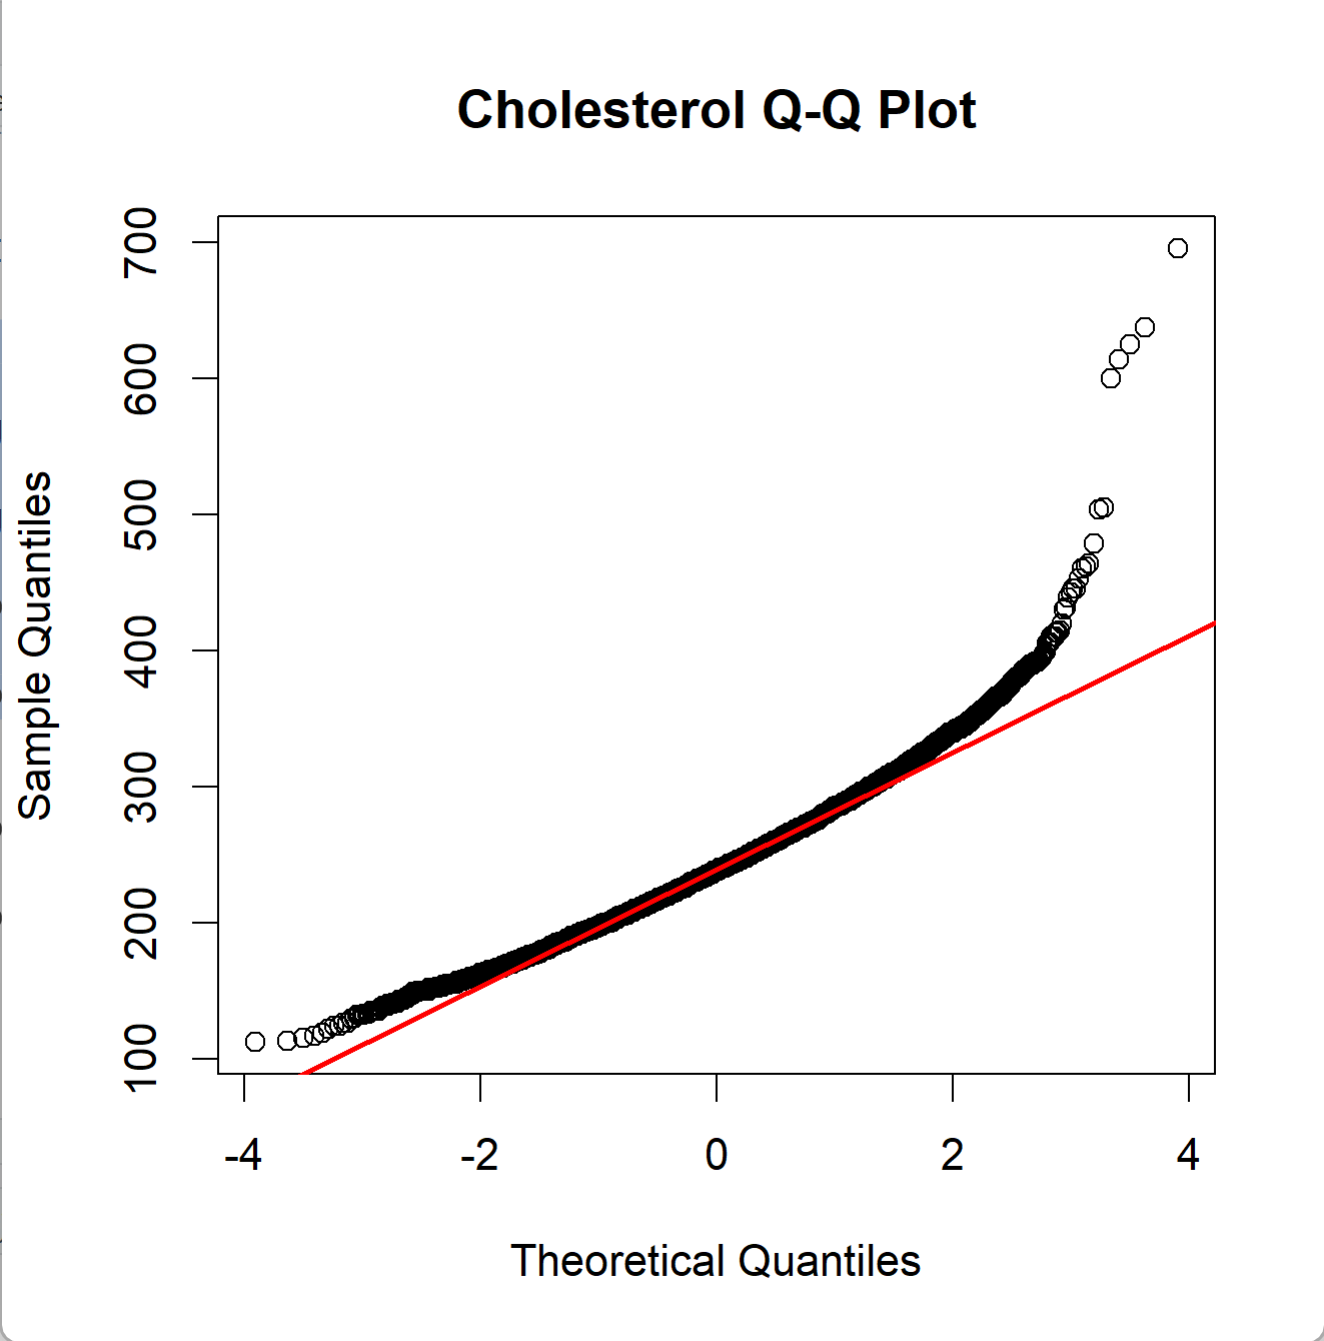
\includegraphics[width=0.8\textwidth]{figs/hw2_qq_cholesterol_original.png}
\end{center}

\begin{center}
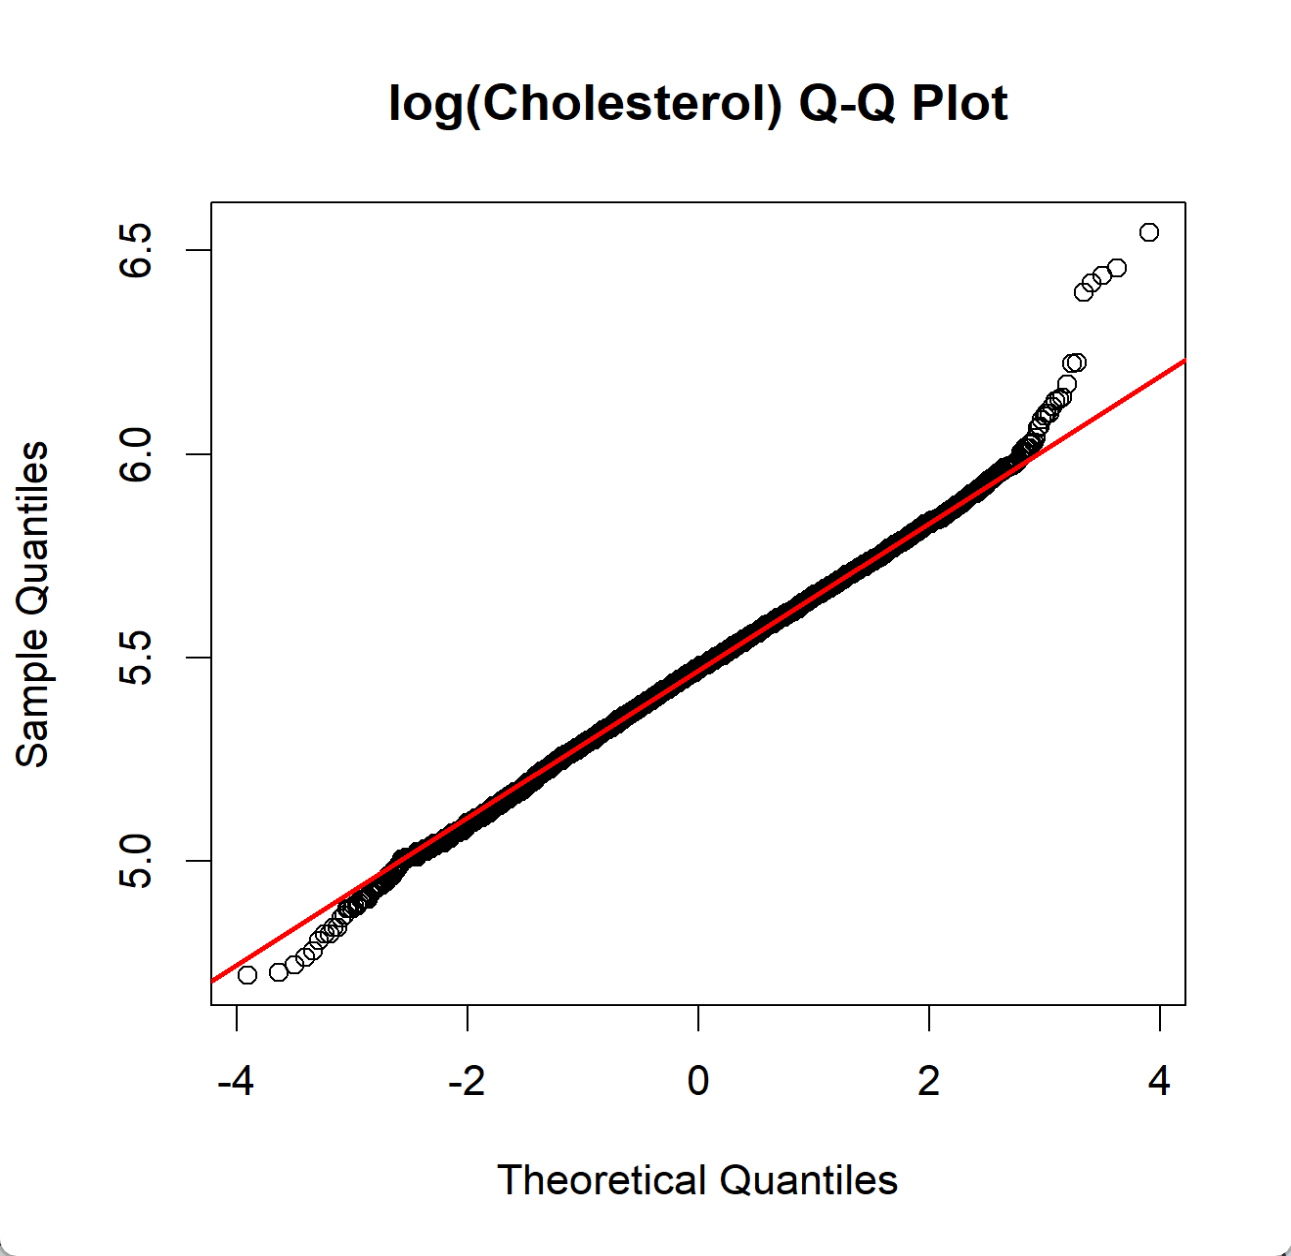
\includegraphics[width=0.8\textwidth]{figs/hw2_qq_cholesterol_log.png}
\end{center}

\begin{center}
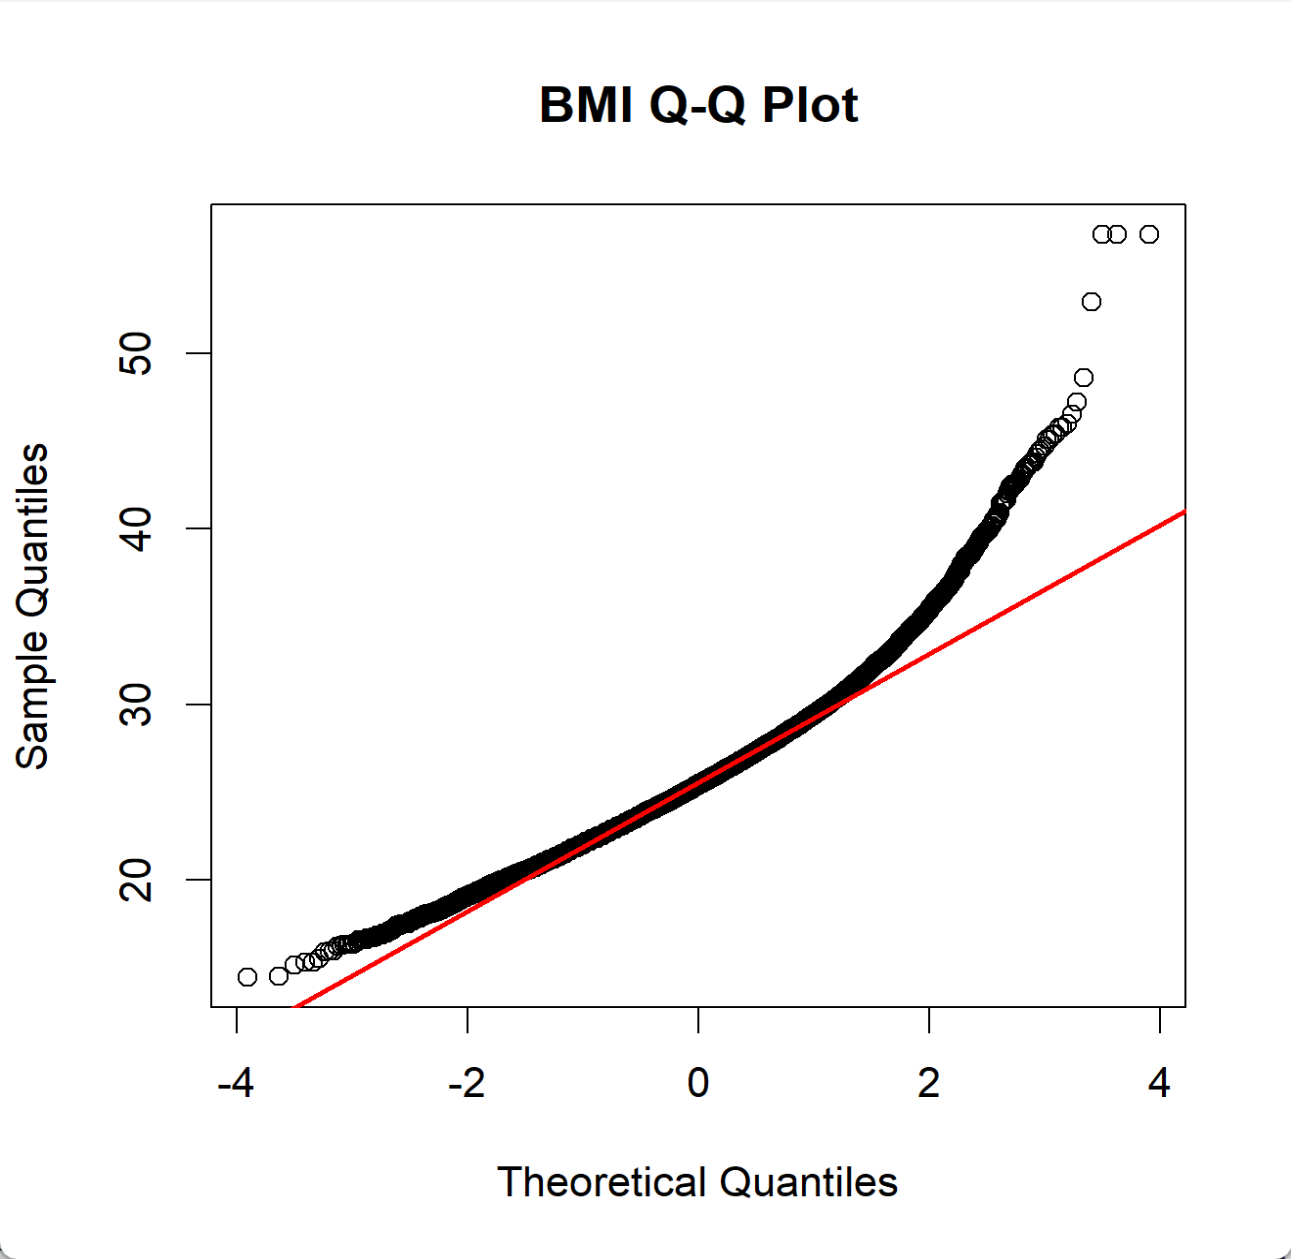
\includegraphics[width=0.8\textwidth]{figs/hw2_qq_bmi_original.png}
\end{center}

\begin{center}
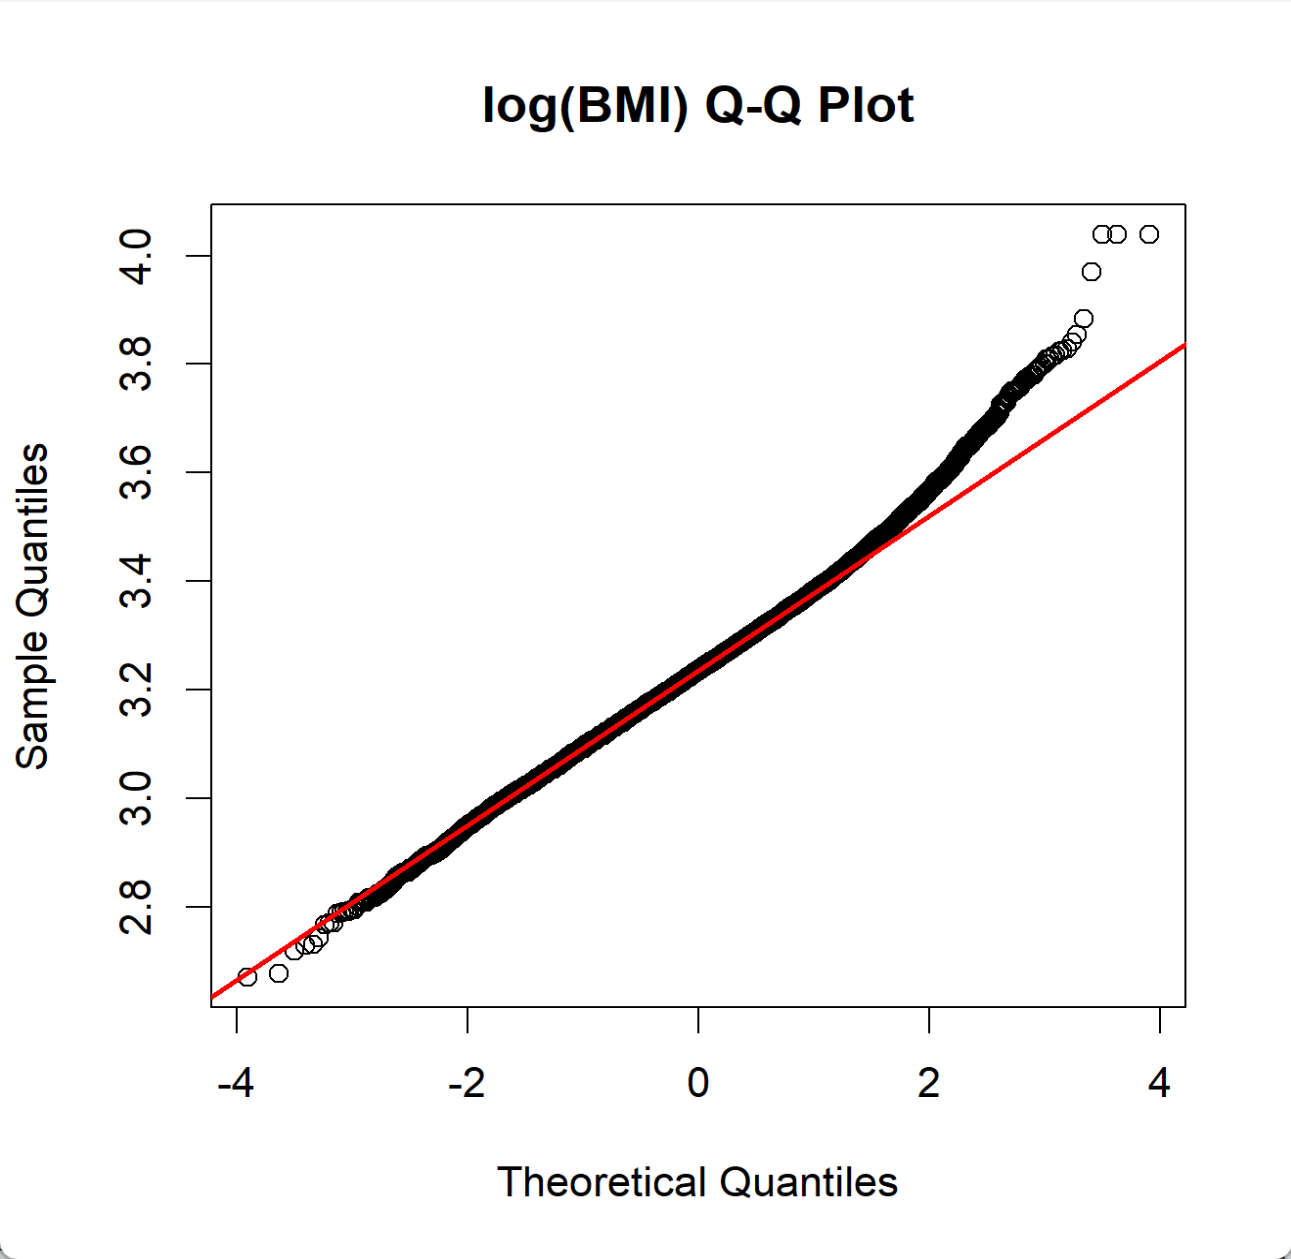
\includegraphics[width=0.8\textwidth]{figs/hw2_qq_bmi_log.png}
\end{center}

\subsubsection*{(c)}

考虑到样本量和可解释性，选用Pearson相关系数对未经变换的原数据进行计算。（在大样本情况下，Pearson 相关系数具有渐近正态性，因此对轻度偏离正态分布的样本具有稳健性，使用是合理的。）

计算得到 $\text{cor} = 0.0758$, 95\%置信区间为 $(0.0569, 0.0946)$, $p$-value $= 3.716 \times 10^{-15}$。有足够证据认为两者存在线性相关的关系，但相关系数数值较小（约 0.076），说明该线性关系在实际意义上比较弱。

此外可以计算 $\text{standard error} = \sqrt{\frac{1 - r^2}{n - 2}} = 0.00963$.

\subsubsection*{(d)}

图中直方图展示了通过 Bootstrap 方法（重复抽样1000次）得到的相关系数的经验分布，虚线表示原始样本计算得到的相关系数。可以看到，bootstrap 分布大致围绕该值对称分布。

\begin{center}
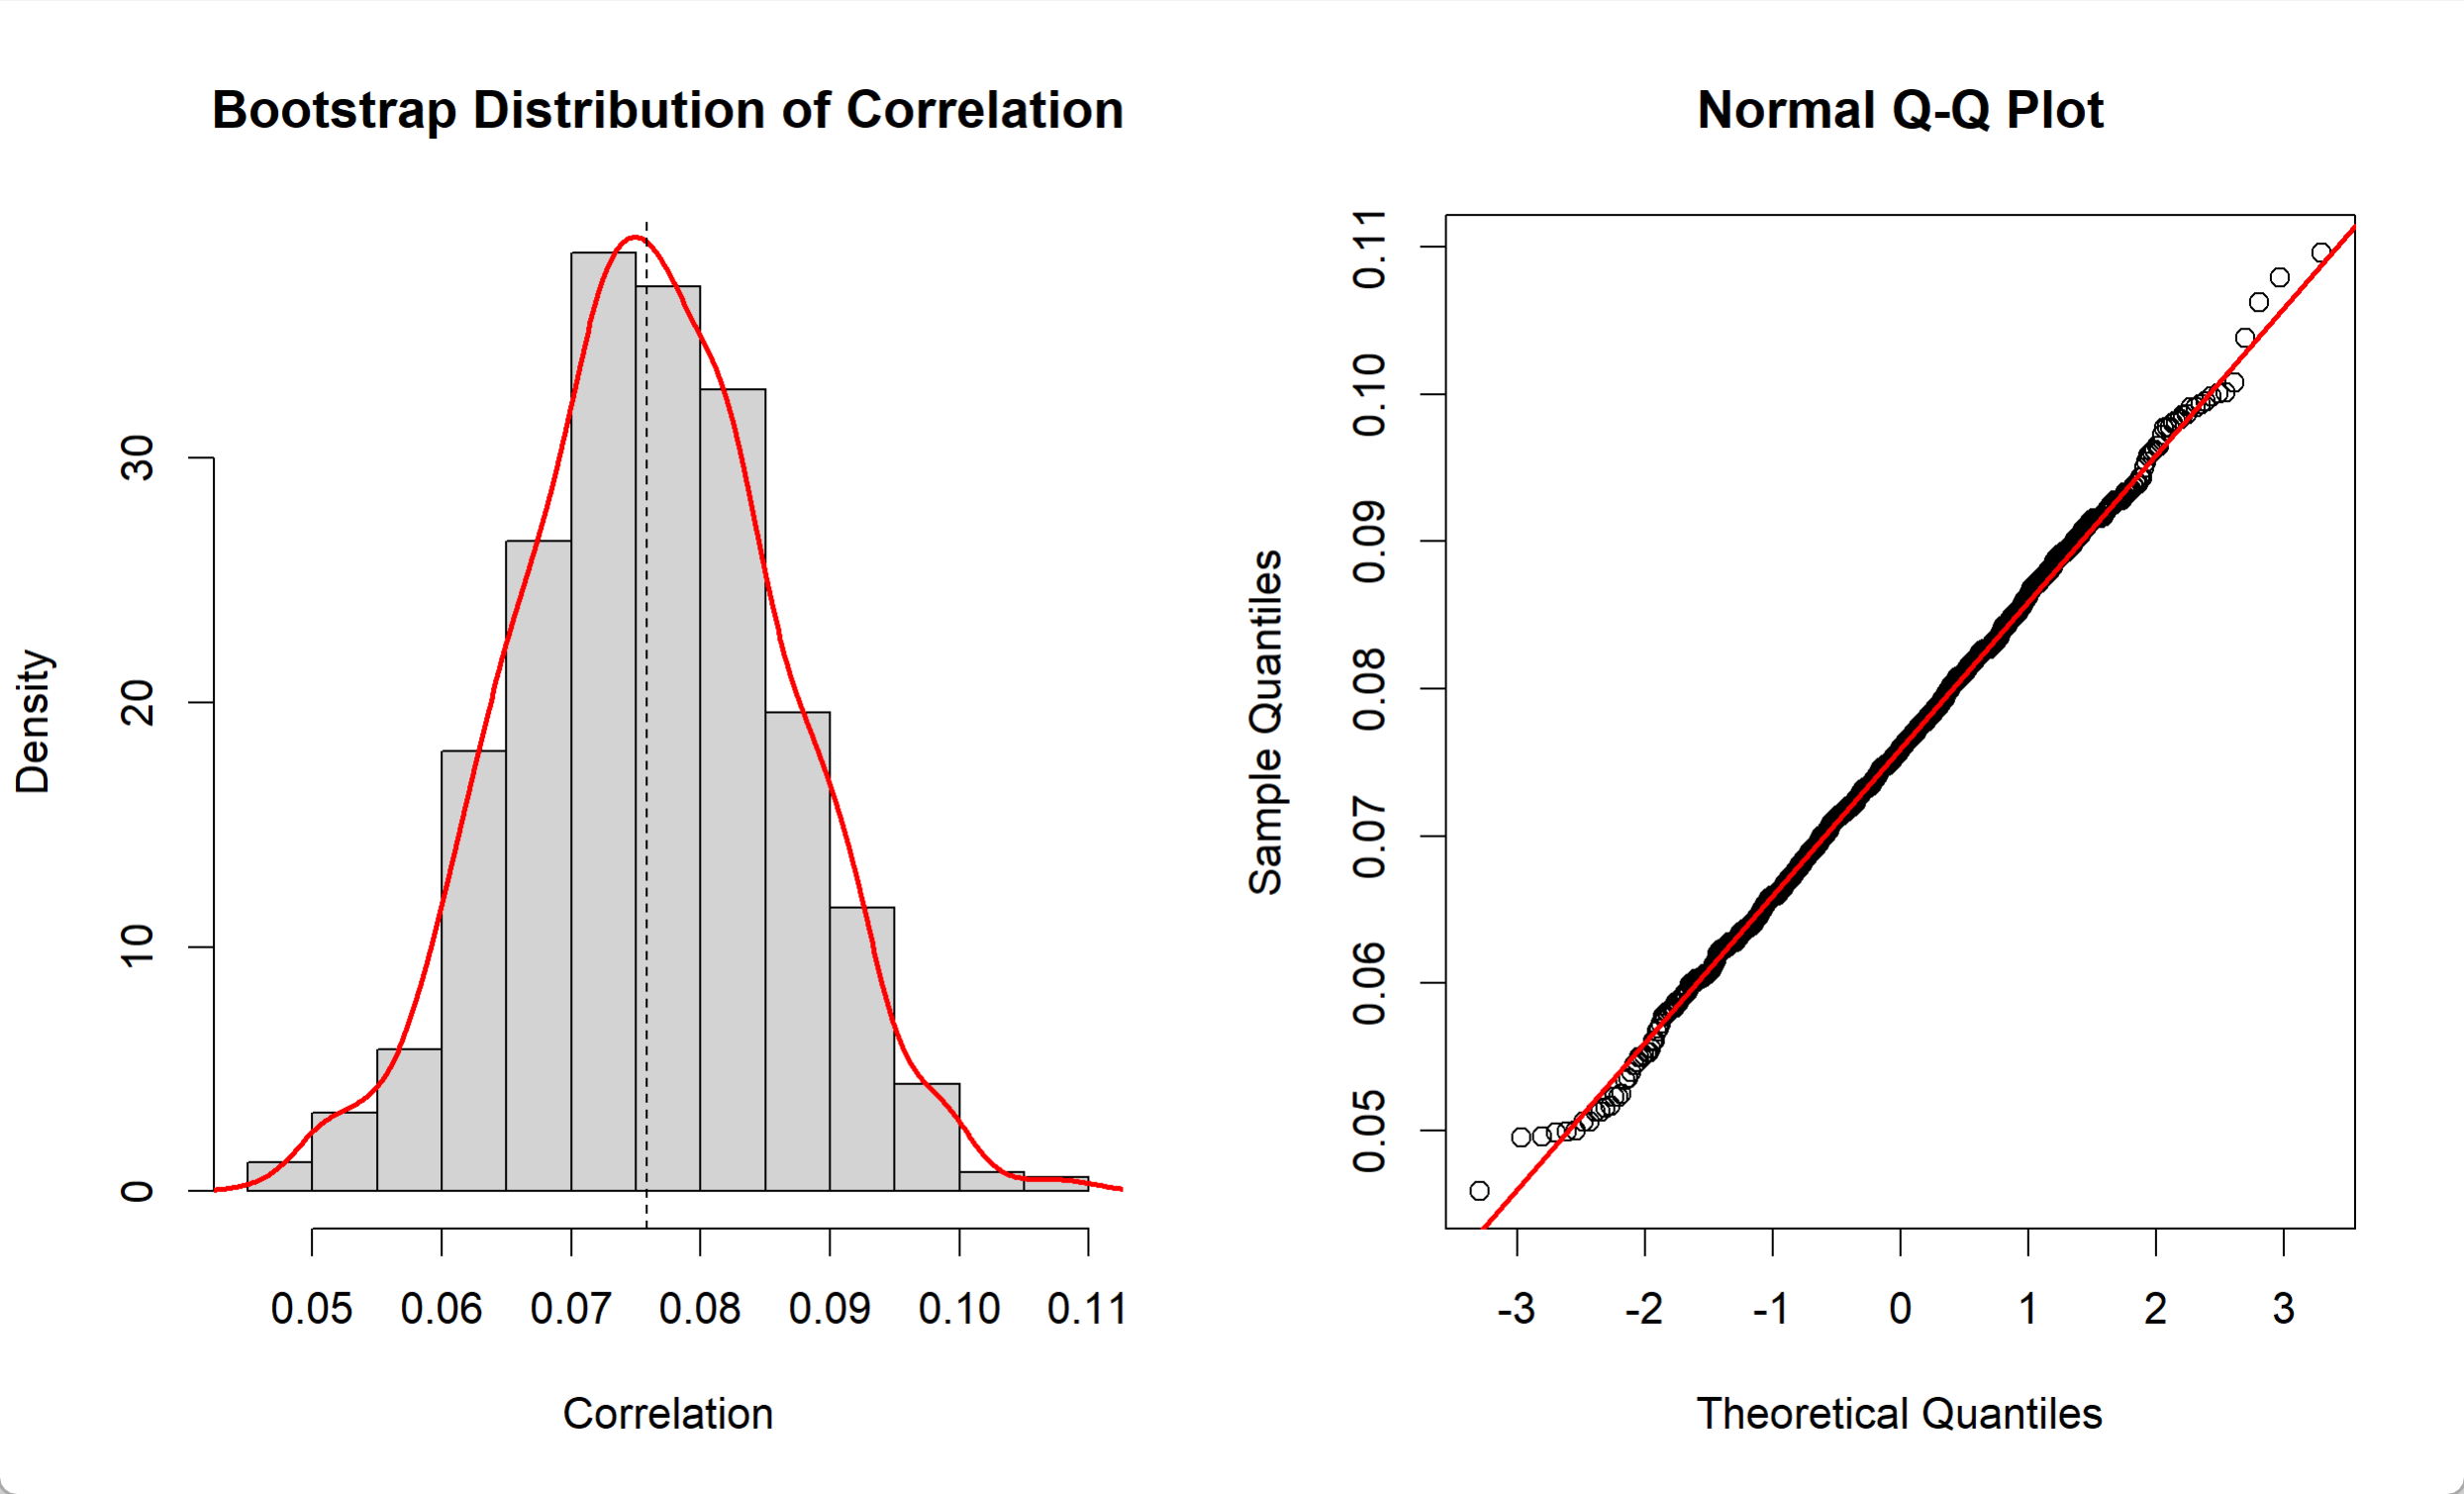
\includegraphics[width=0.8\textwidth]{figs/hw2_bootstrap_distribution.png}
\end{center}

通过直方图和QQ Plot可以看出Bootstrap得到的相关系数分布大致接近正态分布，这与 Pearson 相关系数在大样本下的渐近正态性是相符的。

Bootstrap方法计算的SE为0.0101，与理论计算得到的（0.00963）较为接近。具体地，相对偏差 $\frac{SE_{boot} - SE_{cal}}{SE_{cal}} \times 100\% = 4.88\%$，二者一致性较高。

\textbf{注：}

(1) 本题中对于缺失数据我们采用了删除的处理方式，仅保留BMI和TOTCHOL均有数据的样本（10726个）进行所有小问的分析，保证各问使用的数据一致。

(2) 本题所用代码见下：

\begin{lstlisting}[language=R]
# 6 a&b
df_clean <- df[complete.cases(df[, c("BMI", "TOTCHOL")]), ]
bmi <- df_clean$BMI
totchol <- df_clean$TOTCHOL

qqnorm(bmi, main = "BMI Q-Q Plot")
qqline(bmi, col = "red", lwd = 2)

bmilog <- log(bmi)
qqnorm(bmilog, main = "log(BMI) Q-Q Plot")
qqline(bmilog, col = "red", lwd = 2)

qqnorm(totchol, main = "Cholesterol Q-Q Plot")
qqline(totchol, col = "red", lwd = 2)

totchollog <- log(totchol)
qqnorm(totchollog, main = "log(Cholesterol) Q-Q Plot")
qqline(totchollog, col = "red", lwd = 2)

# 6 c
cor.test(bmi, totchol, method = "pearson")

# 6 d
# bootstrap
B <- 1000
n <- nrow(df_clean)
boot_cor <- numeric(B)
set.seed(100)

for (i in 1:B) {
  idx <- sample(1:n, size = n, replace = TRUE)
  boot_sample <- df_clean[idx, ]
  boot_cor[i] <- cor(boot_sample$BMI, boot_sample$TOTCHOL,
                     method = "pearson")
}
print(sd(boot_cor))

# Plot
par(mfrow = c(1, 2))
hist(boot_cor, freq = FALSE,
     main = "Bootstrap Distribution of Correlation",
     xlab = "Correlation")
lines(density(boot_cor), col = "red", lwd = 2)
abline(v = 0.07583282, lty = 2)

qqnorm(boot_cor)
qqline(boot_cor, col = "red", lwd = 2)
\end{lstlisting}


\newpage

%% ===== HW3 =====
\section{Homework 3: Categorical Data Analysis}

\subsection{Problem 1}

Suppose that all cell counts $\{n_{ij}\}$, $i = 1, \ldots, I$ and $j = 1, \ldots, J$, follow a multinomial distribution with a fixed total count $n$ and proportion parameters $\{\pi_{ij}\}$. Write the likelihood function and solve for the MLE.

\textbf{解答：}

Likelihood:
\[
L(\{\pi_{ij}\}) = \frac{n!}{\prod_{i=1}^{I} \prod_{j=1}^{J} n_{ij}!} \prod_{i=1}^{I} \prod_{j=1}^{J} \pi_{ij}^{n_{ij}}
\]

取对数：
\[
\log L(\{\pi_{ij}\}) = \text{const} + \sum_{i,j} n_{ij} \log \pi_{ij}
\]

已知约束 $\sum_{i,j} \pi_{ij} = 1$，由 Lagrange 乘因子法，令
\[
F = \sum_{i,j} n_{ij} \log \pi_{ij} - \lambda \left(1 - \sum_{i,j} \pi_{ij}\right)
\]

对 $\pi_{ij}$ 求偏导并令其为 0：
\[
\frac{\partial F}{\partial \pi_{ij}} = \frac{n_{ij}}{\pi_{ij}} + \lambda = 0 \implies \pi_{ij} = \frac{n_{ij}}{-\lambda}
\]

对所有 $\pi_{ij}$ 求和：
\[
\sum_{i,j} \pi_{ij} = \frac{\sum_{i,j} n_{ij}}{-\lambda} = \frac{n}{-\lambda} = 1 \implies \lambda = -n
\]

因此：
\[
\boxed{\hat{\pi}_{ij}^{\text{MLE}} = \frac{n_{ij}}{n}, \quad \forall\, i, j}
\]

\subsection{Problem 2}

Verify that the ASE for $\log(\widehat{OR}) = [\log(n_{11}) - \log(n_{12})] - [\log(n_{21}) - \log(n_{22})]$ is
\[
\left(\frac{1}{n_{11}} + \frac{1}{n_{12}} + \frac{1}{n_{21}} + \frac{1}{n_{22}}\right)^{1/2}.
\]

Hint: Note that $n_{11} + n_{12} = n_{1.}$ is a fixed row sum. Consider the function of $n_{11}$:
\[
f(n_{11}) = \log(n_{11}) - \log(n_{1.} - n_{11})
\]

\textbf{解答：}

行和为定值，即 Independent multinomial，$n_{11} \sim B(n_{1.}, p)$。

记 $f(n_{11}) = \log n_{11} - \log(n_{1.} - n_{11})$，则
\[
f'(n_{11}) = \frac{1}{n_{11}} + \frac{1}{n_{1.} - n_{11}} = \frac{1}{n_{11}} + \frac{1}{n_{12}}
\]

由 $n_{11} \sim B(n_{1.}, p)$，$\text{Var}(n_{11}) = n_{1.} p(1-p)$。

由 Delta method：
\[
\text{Var}(f(n_{11})) \approx \left(\frac{1}{n_{11}} + \frac{1}{n_{12}}\right)^2 \cdot n_{1.} p(1-p) \xrightarrow{p} \frac{1}{n_{11}} + \frac{1}{n_{12}}
\]

（当 $n \to \infty$ 时，$\frac{n_{11}}{n_{1.}} \to p$）

同理可得
\[
\text{Var}\left[\log\frac{n_{21}}{n_{22}}\right] \xrightarrow{p} \frac{1}{n_{21}} + \frac{1}{n_{22}}
\]

由于行之间独立，故
\[
\boxed{\text{ASE}\left[\log(\widehat{OR})\right] = \left(\frac{1}{n_{11}} + \frac{1}{n_{12}} + \frac{1}{n_{21}} + \frac{1}{n_{22}}\right)^{1/2}}
\]

\subsection{Problem 3}

Consider three smoking behaviors: nonsmoking, smoking $0 < s < 20$ cigarettes per day, and smoking $s \geq 20$ cigarettes per day. An estimated odds ratio for adult females between the presence of squamous cell carcinoma (yes, no) and smoking behavior (smoking $0 < s < 20$ cigarettes per day, nonsmoking) equals 11.7. The estimated odds ratio for adult females between carcinoma (yes, no) and smoking behavior (smoking $s \geq 20$ cigarettes per day, nonsmoking) is 26.1. Show that the estimated odds ratio between carcinoma (yes, no) and the smoking levels ($s \geq 20$, $0 < s < 20$) equals 2.2. Explain how many odds ratios are needed to characterize such a table.

\textbf{解答：}

\[
OR = \frac{n_{11} n_{22}}{n_{12} n_{21}}
\]

因此
\[
OR_{s \geq 20 \text{ vs } 0 < s < 20} = \frac{OR_{s \geq 20 \text{ vs nonsmoking}}}{OR_{0 < s < 20 \text{ vs nonsmoking}}} = \frac{26.1}{11.7} \approx 2.2
\]

独立的 OR 有 $(2-1) \times (3-1) = \boxed{2}$ 个。由上也可见知道其中 2 个可以算出第 3 个。

（对于 $I \times J$ 列联表，独立 OR 有 $(I-1)(J-1)$ 个。）

\subsection{Problem 4}

A researcher attempts to determine if a disease is associated with the presence of a particular gene. He recruited 250 subjects with the disease and 250 normal subjects. The study results showed that 48 subjects have the gene, among whom 30 were diseased subjects.

\subsubsection*{(a)}

Perform a statistical test to investigate whether the disease is associated with the presence of gene.

\textbf{解答：}

\begin{center}
\begin{tabular}{c|cc|c}
 & gene: yes & gene: no & total \\
\hline
disease: yes & 30 & 220 & 250 \\
disease: no & 18 & 232 & 250 \\
\hline
total & 48 & 452 & 500 \\
\end{tabular}
\end{center}

使用 Pearson $\chi^2$ test：$H_0: \pi_{ij} = \pi_{i.} \cdot \pi_{.j}$, $\forall\, i\ \&\ j$, $\alpha = 0.05$

Expected counts：
\[
\hat{\mu}_{11} = \frac{48 \times 250}{500} = 24 = \hat{\mu}_{21}
\]
\[
\hat{\mu}_{12} = \frac{452 \times 250}{500} = 226 = \hat{\mu}_{22}
\]

Statistic：
\[
\chi^2 = \frac{(30 - 24)^2}{24} + \frac{(220 - 226)^2}{226} + \frac{(18 - 24)^2}{24} + \frac{(232 - 226)^2}{226} = 3.32
\]

$\chi^2 \sim \chi^2(1)$，对应临界值 $\chi^2_{0.05}(1) = 3.84 > 3.32$

因此 \textbf{不拒绝 $H_0$}，没有足够理由说明疾病与该基因相关。

\subsubsection*{(b)}

Suppose that we know the following additional information: each of the 250 normal subjects was matched to each of the 250 diseased subjects by gender, race and age group; for 214 matched pairs, neither the diseased subject nor their matched normal subject has the gene. Perform an appropriate statistical test to investigate whether the disease is associated with the presence of the gene.

\textbf{解答：}

\begin{center}
\begin{tabular}{c|cc|c}
 & normal: no & normal: yes & total \\
\hline
disease: no & 214 & 6 & 220 \\
disease: yes & 18 & 12 & 30 \\
\hline
total & 232 & 18 & 250 \\
\end{tabular}
\end{center}

$H_0$ 同 (a)。根据配对数据可以构建如下列联表，使用 McNemar test：
\[
\chi^2 = \frac{(18 - 6)^2}{18 + 6} = \frac{144}{24} = 6 > 3.84
\]
\[
\Rightarrow \text{拒绝 } H_0
\]

认为疾病和基因可能相关。

\subsubsection*{(c)}

Compare the test results in (a) and (b) and explain why they are different.

\textbf{解答：}

解释：未配对时可能忽略了 gender, race, age 等可能的协变量对结果的影响，而配对则考虑了这些信息，增强了 power。

\subsection{Problem 5}

(Framingham study) Consider the binary cholesterol status as the outcome. Test its independence with BMI, age group, and sex, separately, at baseline. For each test, follow the steps below.

(a) Visualize the data using figures or tables.

(b) Specify your selected method and report your $p$-value.

(c) Interpret your results.

\subsubsection*{1. BMI（分组）}

\begin{center}
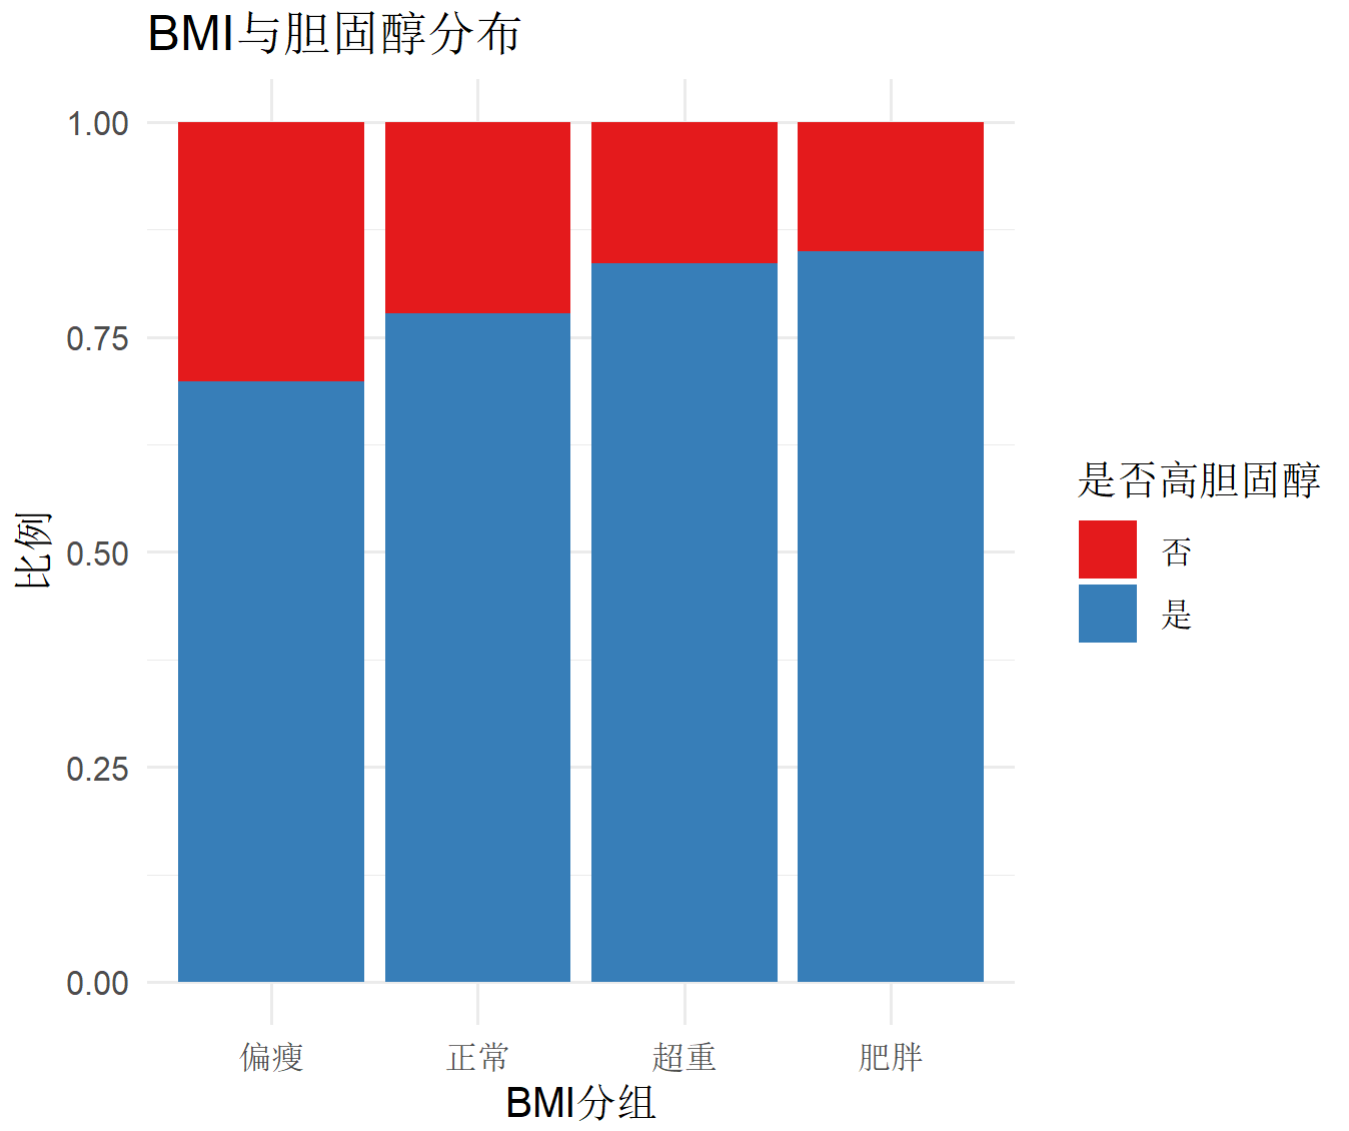
\includegraphics[width=0.7\textwidth]{figs/hw3_bmi_cholesterol_bar.png}
\end{center}

\begin{center}
\begin{tabular}{l|ccc}
 & 胆固醇 0 & 胆固醇 1 & Sum \\
\hline
偏瘦 & 48 & 111 & 159 \\
正常 & 783 & 2735 & 3518 \\
超重 & 720 & 3670 & 4390 \\
肥胖 & 399 & 2260 & 2659 \\
\hline
Sum & 1950 & 8776 & 10726 \\
\end{tabular}
\end{center}

使用 Pearson's Chi-squared test, $p\text{-value} < 2.2 \times 10^{-16}$

\subsubsection*{2. Age group}

\begin{center}
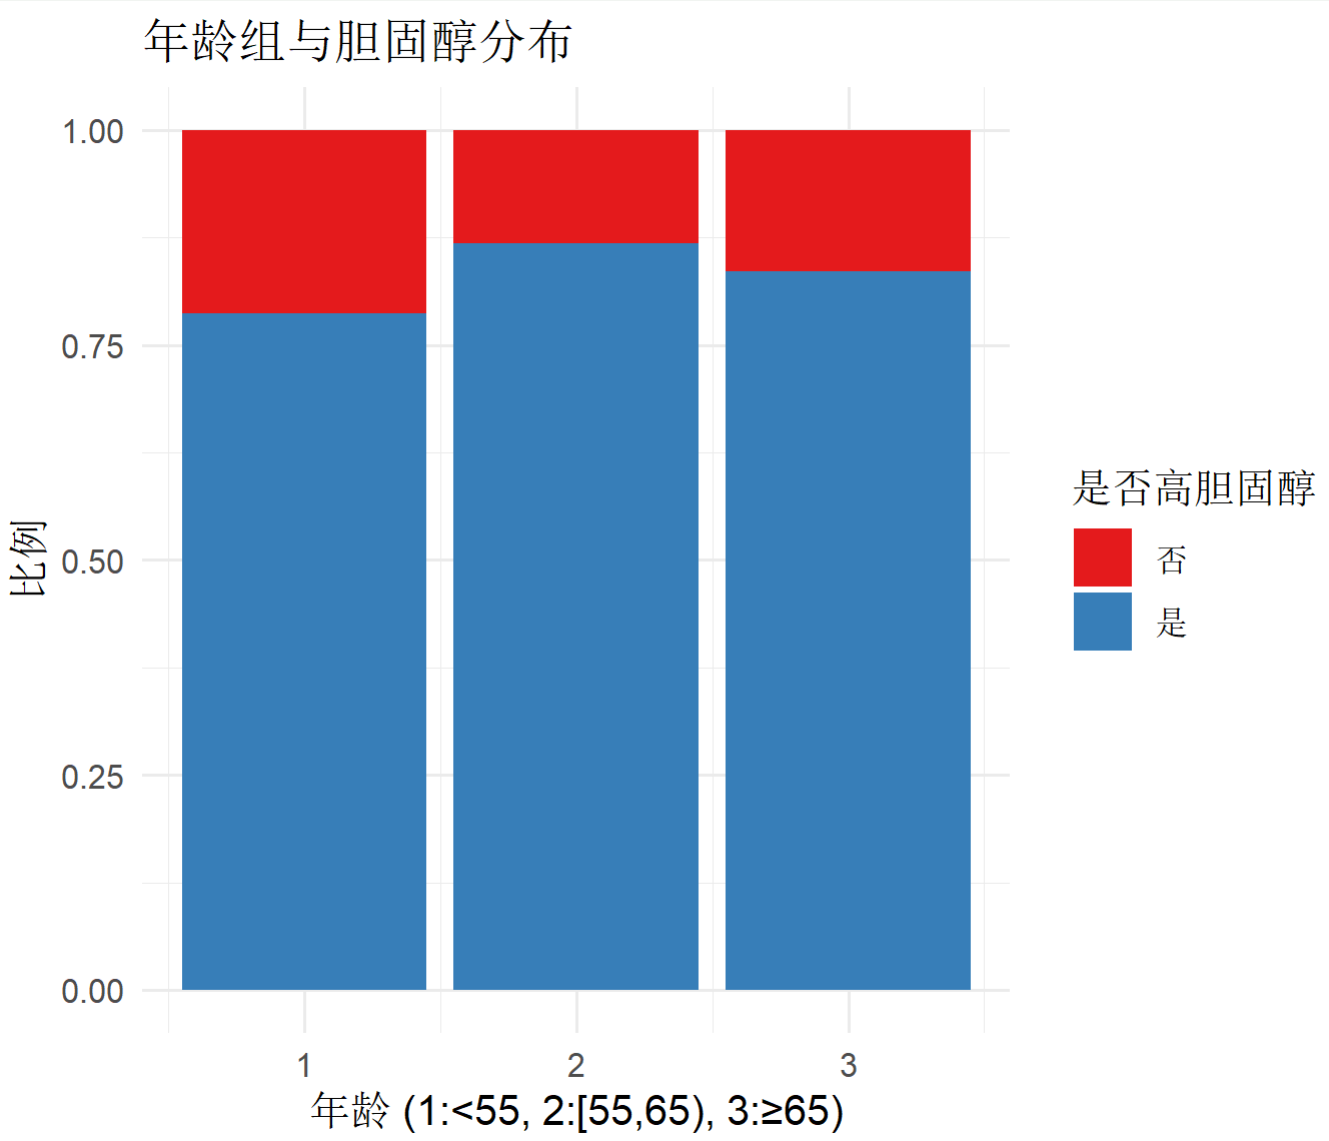
\includegraphics[width=0.7\textwidth]{figs/hw3_age_cholesterol_bar.png}
\end{center}

\begin{center}
\begin{tabular}{l|ccc}
 & totchol 0 & totchol 1 & Sum \\
\hline
1 ($<55$) & 1281 & 4716 & 5997 \\
2 ($[55,65)$) & 424 & 2809 & 3233 \\
3 ($\geq 65$) & 245 & 1251 & 1496 \\
\hline
Sum & 1950 & 8776 & 10726 \\
\end{tabular}
\end{center}

使用 Pearson's Chi-squared test, $p\text{-value} < 2.2 \times 10^{-16}$

\subsubsection*{3. Sex}

\begin{center}
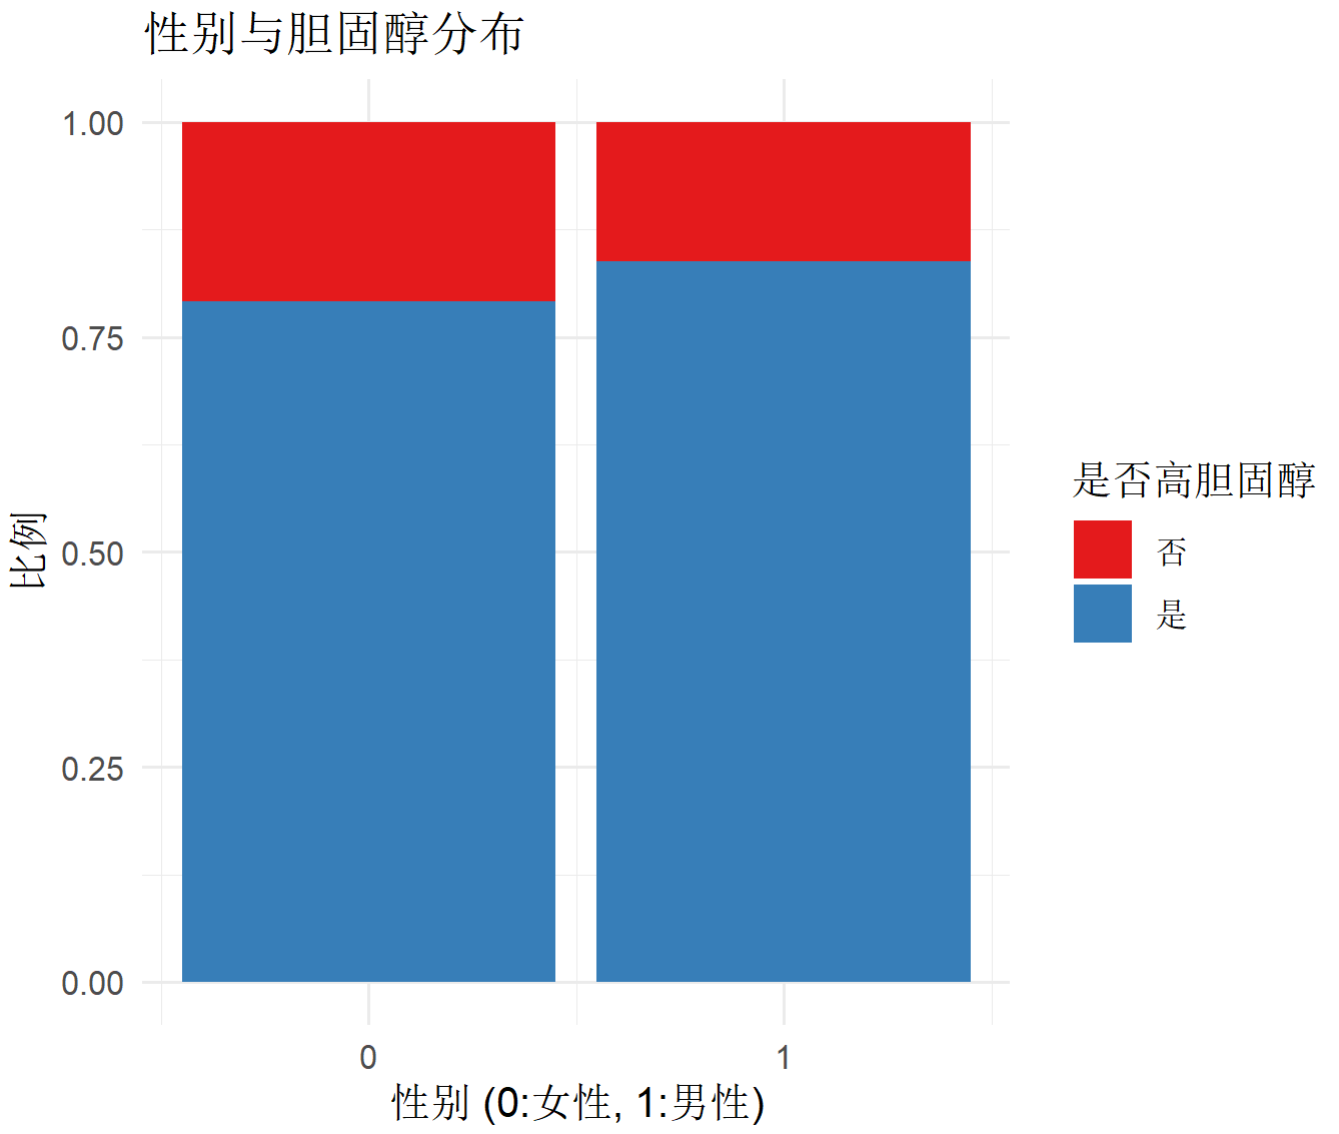
\includegraphics[width=0.7\textwidth]{figs/hw3_sex_cholesterol_bar.png}
\end{center}

\begin{center}
\begin{tabular}{l|ccc}
 & totchol 0 & totchol 1 & Sum \\
\hline
0 (female) & 967 & 3665 & 4632 \\
1 (male) & 983 & 5111 & 6094 \\
\hline
Sum & 1950 & 8776 & 10726 \\
\end{tabular}
\end{center}

使用 Pearson's Chi-squared test, $p\text{-value} = 3.23 \times 10^{-10}$

\subsubsection*{(c) Interpret}

以上三组均有 $p\text{-value} < 0.05$，拒绝零假设，即认为比较的两组变量有相关性。具体地，BMI 大的人比 BMI 小的人更可能有高胆固醇，老年人群比较年轻的人群更可能有高胆固醇，男性比女性更可能有高胆固醇。

此外，由于 BMI 的取值为连续变量，又在次前作业里检验过 BMI 的分布严重偏离正态，故我们可以选用 Wilcoxon rank sum test。

\begin{center}
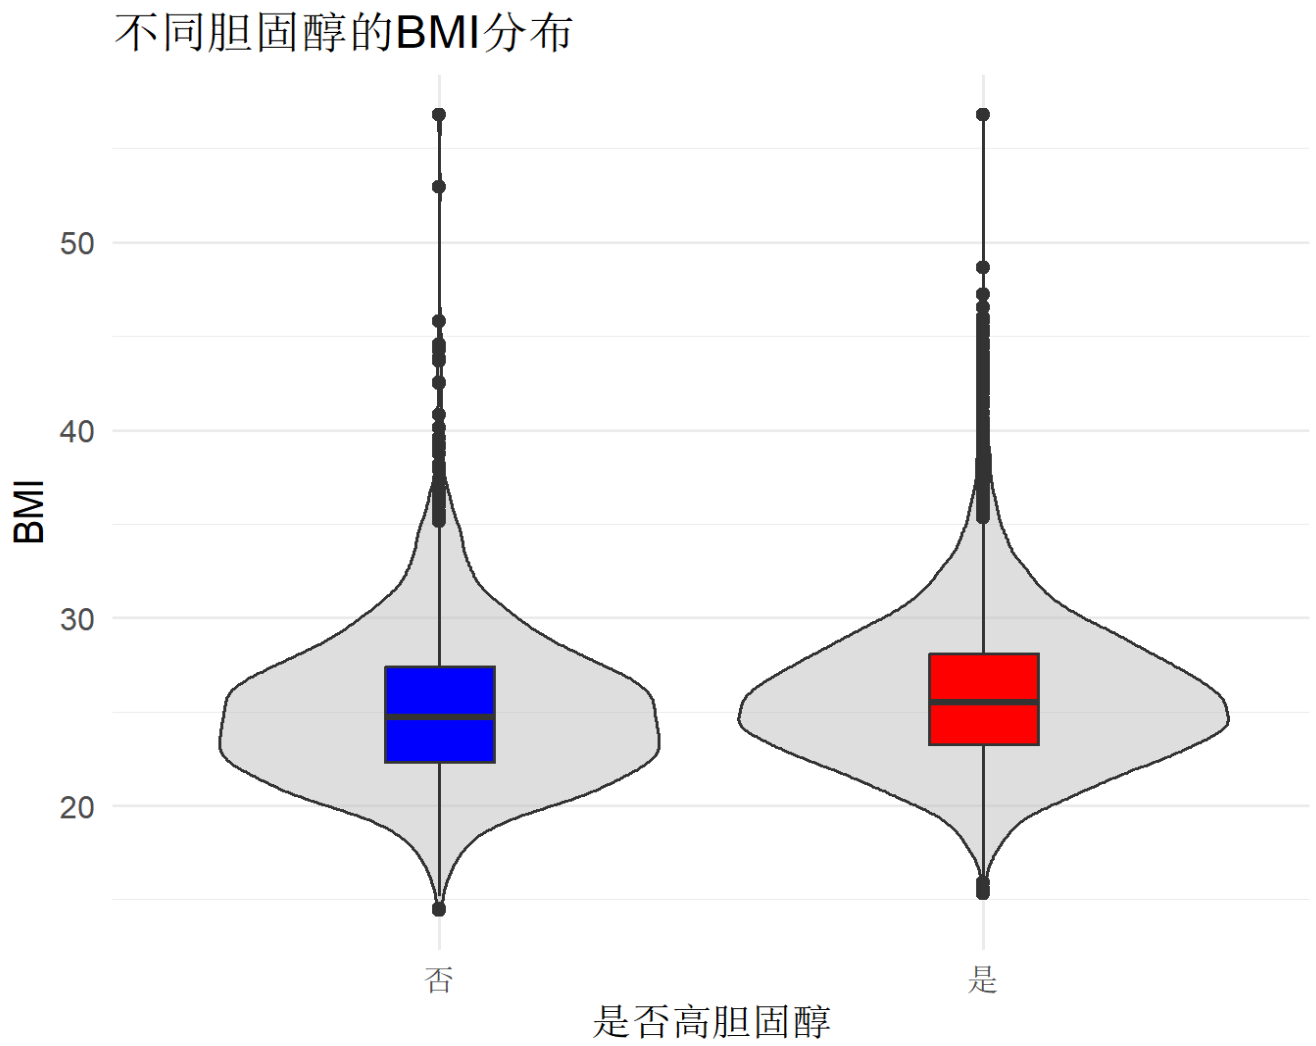
\includegraphics[width=0.7\textwidth]{figs/hw3_bmi_violin.png}
\end{center}

Wilcoxon rank sum test 结果：
\begin{verbatim}
p-value < 2.2e-16
alternative hypothesis: true location shift is not equal to 0
\end{verbatim}

\textbf{注：}

1. 对所用列的缺失数据采取了整行删除处理。

2. 前面部分如果否用蓝色是用红色可能更符合直觉，但因为还是不熟悉 ggplot，本次作业先不修改了。

3. 代码见下：

\begin{lstlisting}[language=R]
library(ggplot2)
df <- read.csv("Framingham_data.csv")
dfclean <- df[!is.na(df$TOTCHOL) & !is.na(df$BMI)
              & !is.na(df$AGE_group) & !is.na(df$SEX), ]
dfclean$bi_chole <- ifelse(dfclean$TOTCHOL > 200, 1, 0)

# a visualize (figures & tables)
# BMI (BMI也分组)
dfclean$bmigroup <- cut(
  dfclean$BMI,
  breaks = c(-Inf, 18.5, 24, 28, Inf),
  labels = c("偏瘦", "正常", "超重", "肥胖")
)
ggplot(dfclean, aes(x = bmigroup, fill = factor(bi_chole))) +
  geom_bar(position = "fill") +
  labs(title = "BMI与胆固醇分布",
       x = "BMI分组", y = "比例", fill = "是否高胆固醇") +
  scale_fill_brewer(labels = c("否", "是"), palette = "Set1") +
  theme_minimal()

b <- table("BMI" = dfclean$bmigroup,
           "胆固醇" = dfclean$bi_chole)
addmargins(b)
chisq.test(b)

# age
ggplot(dfclean, aes(x = AGE_group, fill = factor(bi_chole))) +
  geom_bar(position = "fill") +
  labs(title = "年龄组与胆固醇分布",
       x = "年龄 (1:<55, 2:[55,65), 3:≥65)",
       y = "比例", fill = "是否高胆固醇") +
  scale_fill_brewer(labels = c("否", "是"), palette = "Set1") +
  theme_minimal()

a <- table("age group" = dfclean$AGE_group,
           "totchol" = dfclean$bi_chole)
addmargins(a)
chisq.test(a)

# sex
ggplot(dfclean, aes(x = SEX, fill = factor(bi_chole))) +
  geom_bar(position = "fill") +
  labs(title = "性别与胆固醇分布",
       x = "性别 (0:女性, 1:男性)", y = "比例",
       fill = "是否高胆固醇") +
  scale_fill_brewer(labels = c("否", "是"), palette = "Set1") +
  scale_x_continuous(breaks = c(0, 1)) +
  theme_minimal()

s <- table("sex" = dfclean$SEX,
           "totchol" = dfclean$bi_chole)
addmargins(s)
chisq.test(s)

# 连续BMI
ggplot(dfclean, aes(x = factor(bi_chole, labels = c("否","是")),
                    y = BMI)) +
  geom_violin(fill = "gray", alpha = 0.5) +
  geom_boxplot(fill = c("blue", "red"), width = 0.2) +
  labs(title = "不同胆固醇的BMI分布",
       x = "是否高胆固醇", y = "BMI") +
  theme_minimal()
wilcox.test(dfclean$BMI ~ dfclean$bi_chole)
\end{lstlisting}


\newpage

%% ===== HW4 =====
\section{Homework 4: Linear Models}
\subsection{Problem 1}

In a simple linear regression with one covariate $X_i$:

\subsection*{(a)}

Show that the estimates for the slope and intercept are
\[
\widehat{\beta} = \frac{\sum_{i=1}^{n}(X_i - \overline{X}_n)(Y_i - \overline{Y}_n)}{\sum_{i=1}^{n}(X_i - \overline{X}_n)^2}
\]
and
\[
\widehat{\alpha} = \overline{Y}_n - \widehat{\beta}\overline{X}_n.
\]

Hint:
\[
\begin{pmatrix} a & b \\ b & c \end{pmatrix}^{-1} = \frac{1}{ac - b^2} \begin{pmatrix} c & -b \\ -b & a \end{pmatrix}
\]

\textbf{Solution.}

设简单线性回归模型为 $Y_i = \beta X_i + \alpha + \varepsilon_i$，拟合值为 $\widehat{Y} = \widehat{\beta} X + \widehat{\alpha}$。

最小二乘法的目标是最小化残差平方和：
\[
\sum_{i=1}^{n}(Y_i - \alpha - \beta X_i)^2
\]

对 $\alpha$ 求偏导并令其为0：
\[
\frac{\partial}{\partial \alpha} = -2\sum_{i=1}^{n}(Y_i - \alpha - \beta X_i) = 0
\]
\[
\Rightarrow \sum_{i=1}^{n} Y_i - n\alpha - \beta\sum_{i=1}^{n} X_i = 0
\]
\[
\Rightarrow \widehat{\alpha} = \overline{Y} - \beta\overline{X}
\]

对 $\beta$ 求偏导并令其为0：
\[
\frac{\partial}{\partial \beta} = -2\sum_{i=1}^{n} X_i(Y_i - \alpha - \beta X_i) = 0
\]
\[
\Rightarrow \sum_{i=1}^{n} X_i Y_i - \alpha\sum_{i=1}^{n} X_i - \beta\sum_{i=1}^{n} X_i^2 = 0
\]

将上述两个方程写成矩阵形式：
\[
\begin{pmatrix} n & \sum X_i \\ \sum X_i & \sum X_i^2 \end{pmatrix} \begin{pmatrix} \alpha \\ \beta \end{pmatrix} = \begin{pmatrix} \sum Y_i \\ \sum X_i Y_i \end{pmatrix}
\]

解得：
\[
\begin{pmatrix} \widehat{\alpha} \\ \widehat{\beta} \end{pmatrix} = \frac{1}{n\sum X_i^2 - (\sum X_i)^2} \begin{pmatrix} \sum X_i^2 & -\sum X_i \\ -\sum X_i & n \end{pmatrix} \begin{pmatrix} \sum Y_i \\ \sum X_i Y_i \end{pmatrix}
\]

因此：
\[
\widehat{\beta} = \frac{-\sum X_i \sum Y_i + n\sum X_i Y_i}{n\sum X_i^2 - (\sum X_i)^2}
\]

整理（同除以 $n$）：
\[
\widehat{\beta} = \frac{\sum_{i=1}^{n}(X_i - \overline{X})(Y_i - \overline{Y})}{\sum_{i=1}^{n}(X_i - \overline{X})^2}
\]

\hfill $\blacksquare$

\subsection*{(b)}

Show that $R^2$ is the squared Pearson's correlation between $Y_i$'s and $X_i$'s.

\textbf{Solution.}

已知：
\[
R^2 = \frac{\sum(\widehat{Y}_i - \overline{Y})^2}{\sum(Y_i - \overline{Y})^2}, \quad \text{Cor}(X,Y) = \frac{[\sum(X_i - \overline{X})(Y_i - \overline{Y})]^2}{\sum(X_i - \overline{X})^2 \sum(Y_i - \overline{Y})^2}
\]

由 $\widehat{Y}_i = \widehat{\alpha} + \widehat{\beta} X_i$，可得：
\[
\sum(\widehat{Y}_i - \overline{Y})^2 = \sum[\widehat{\alpha} + \widehat{\beta} X_i - \widehat{\alpha} - \widehat{\beta}\overline{X}]^2 = \widehat{\beta}^2 \sum(X_i - \overline{X})^2
\]

又因为：
\[
\sum(X_i - \overline{X})(Y_i - \overline{Y}) = \sum(X_i - \overline{X})(\widehat{\alpha} + \widehat{\beta} X_i - \widehat{\alpha} - \widehat{\beta}\overline{X}) = \widehat{\beta}\sum(X_i - \overline{X})^2
\]

代入上式，则：
\[
R^2 = \widehat{\beta}^2 \frac{\sum(X_i - \overline{X})^2}{\sum(Y_i - \overline{Y})^2}
\]

因此：
\[
\text{Cor}(X,Y) = \frac{\widehat{\beta}^2 [\sum(X_i - \overline{X})^2]^2}{\sum(X_i - \overline{X})^2 \sum(Y_i - \overline{Y})^2} = \widehat{\beta}^2 \frac{\sum(X_i - \overline{X})^2}{\sum(Y_i - \overline{Y})^2} = R^2
\]

\hfill $\blacksquare$

\newpage

\subsection{Problem 2}

(Framingham study) Consider the \textbf{log-transformed cholesterol level} as the outcome.

\subsection*{(a)}

Fit a \textbf{linear model} of the outcome on one covariate, \textbf{BMI}.

\subsubsection*{(i)}

Test the null hypothesis of no BMI effect. Visualize the data to check their relationship.

\textbf{Solution.}

符号同problem 1，结果如下：
\[
\widehat{\alpha} = 5.37, \quad \widehat{\beta} = 0.00364
\]

$p\text{-value} < 2 \times 10^{-16}$，拒绝原假设。

\begin{center}
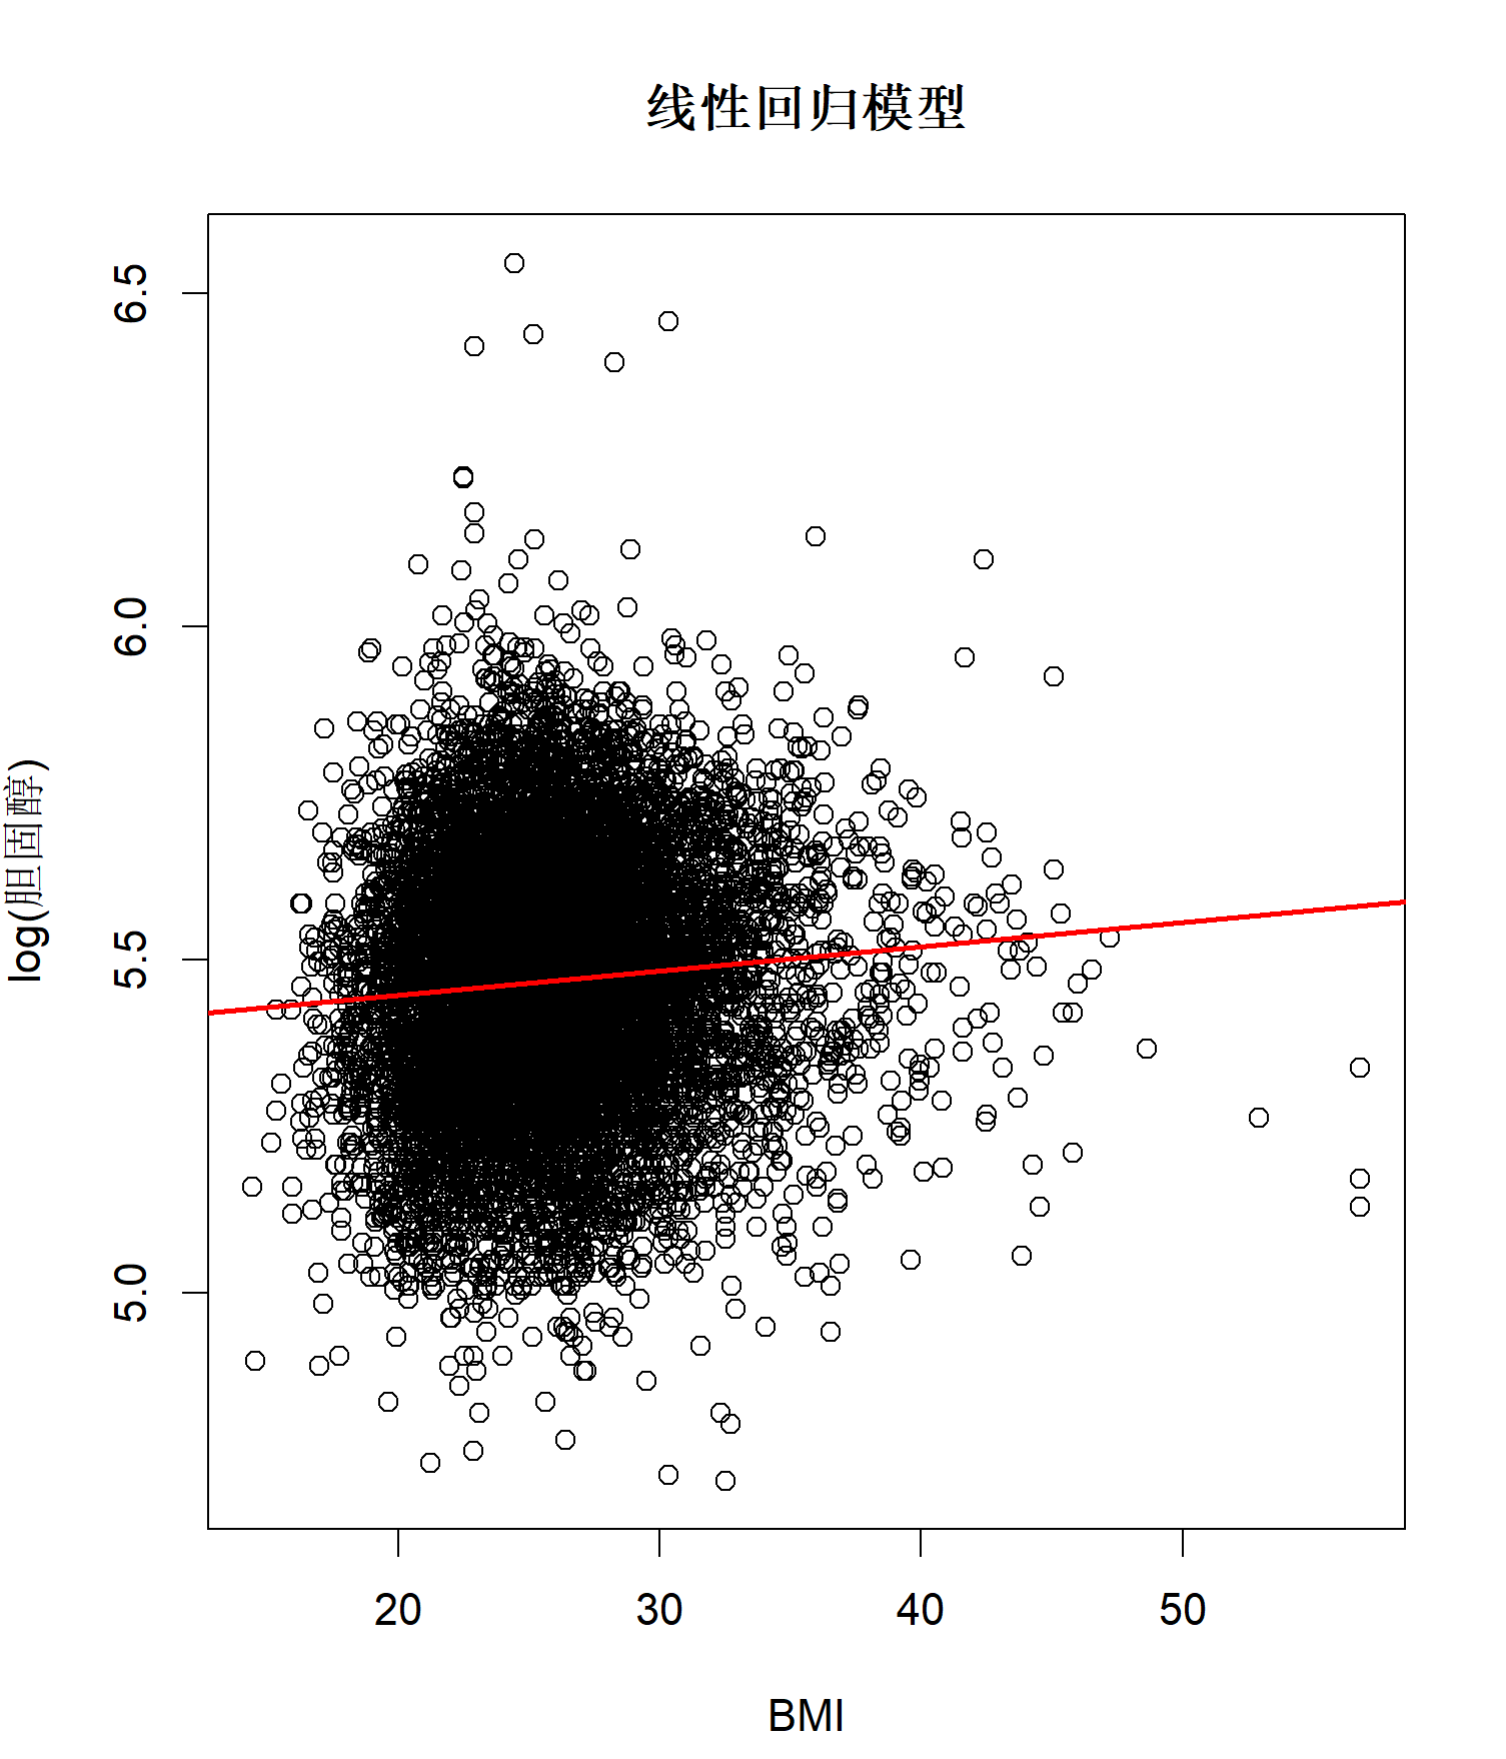
\includegraphics[width=0.7\textwidth]{figs/hw4_bmi_logcholesterol_scatter.png}
\end{center}

图中可以看出二者正相关。

\subsubsection*{(ii)}

Report the $R^2$ value and verify that it is the squared Pearson correlation when there is only one predictor.

\textbf{Solution.}

$R^2 = 0.006311$

$\rho^2 = 0.006311$，本问在problem 1的基础上用数据验证了 $R^2 = \rho^2$。

remark：数据点很多，虽然这里 $R^2$ 十分小但是仍然可以有显著相关性。

\subsubsection*{(iii)}

Plot the residuals to check:
\begin{itemize}
    \item whether the linear model is correctly specified,
    \item whether the errors are normal and homogeneous,
    \item whether there is any outlier.
\end{itemize}

\textbf{Solution.}

\begin{center}
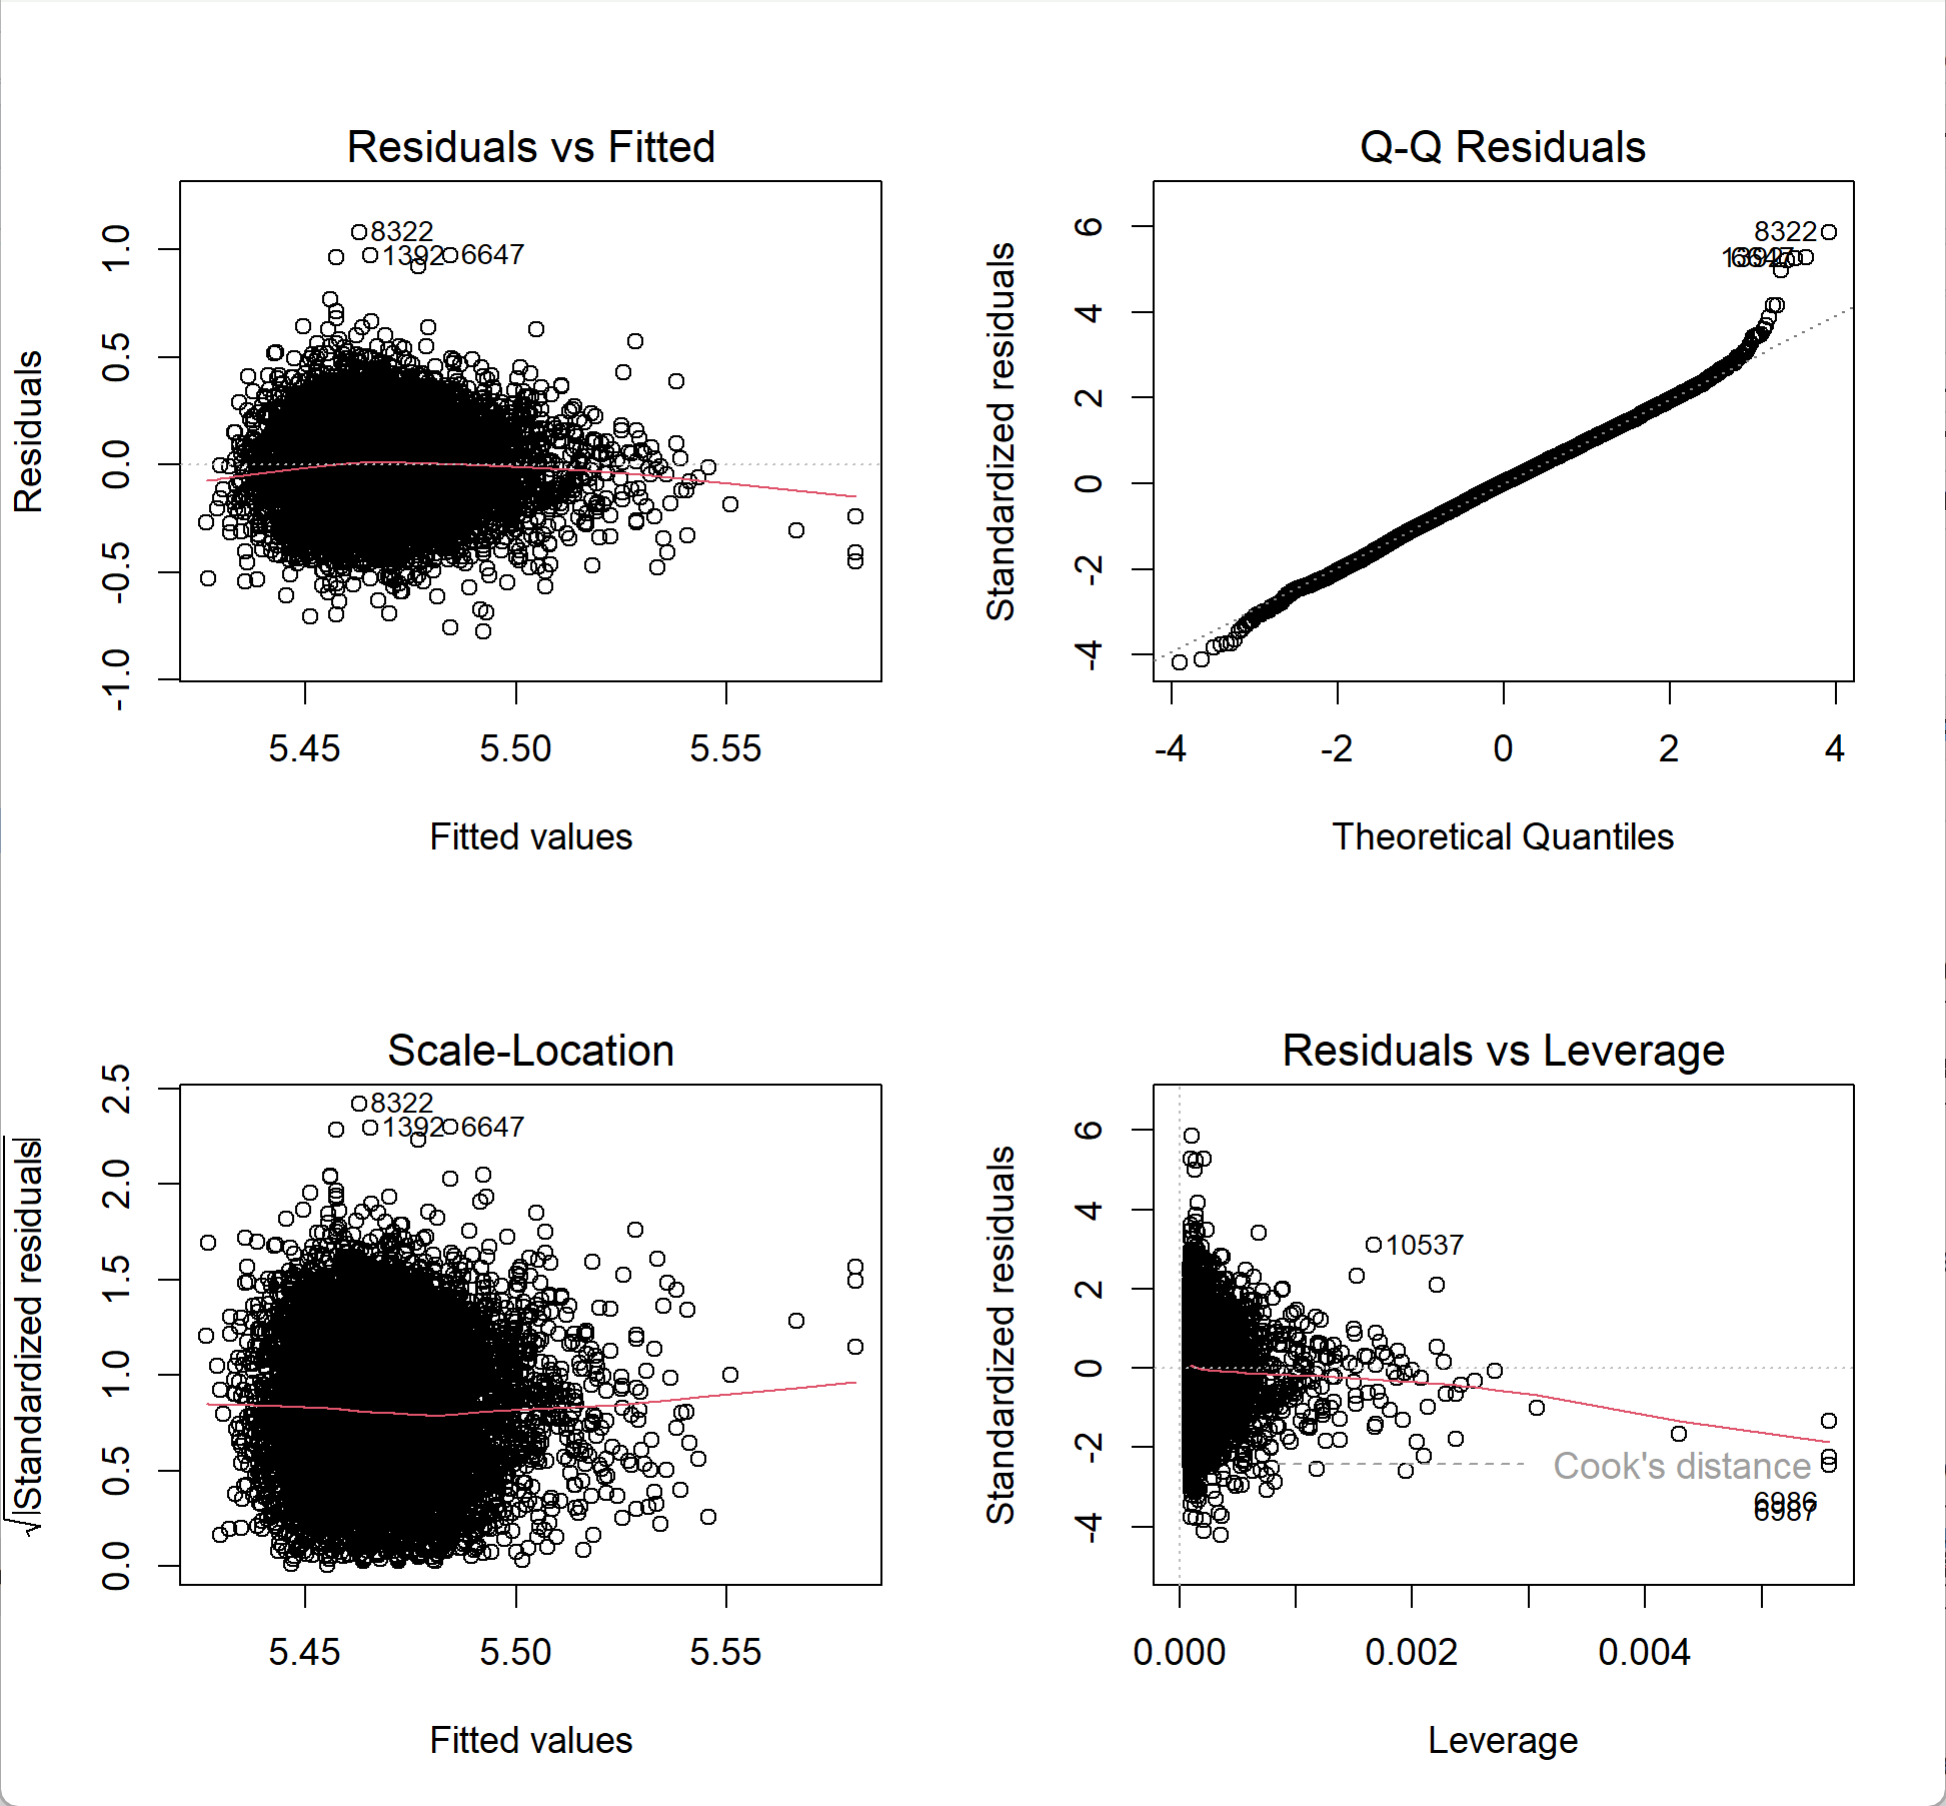
\includegraphics[width=0.8\textwidth]{figs/hw4_bmi_residuals.png}
\end{center}

\begin{itemize}
    \item 基本正确，Residuals vs Fitted 图中残差拟合线虽然有一定弧度但均接近0；残差在0两侧分布基本均匀。scale-location 图拟合线基本水平，没有出现明显的异方差情况。说明对线性模型的假设基本正确。
    \item 根据Q-Q Residuals 图，误差基本服从正态分布，但右尾有一定偏移，说明数据虽然经过对数变换但仍然存在重尾现象。
    \item 有极少的离群值，已在图中标注。
\end{itemize}

综上，使用线性模型是合理的。

\subsection*{(b)}

Fit an \textbf{ANOVA} model of the outcome on \textbf{age group}.

\subsubsection*{(i)}

Test the null hypothesis of no age effect. Visualize the data to check their relationship.

\textbf{Solution.}

\begin{center}
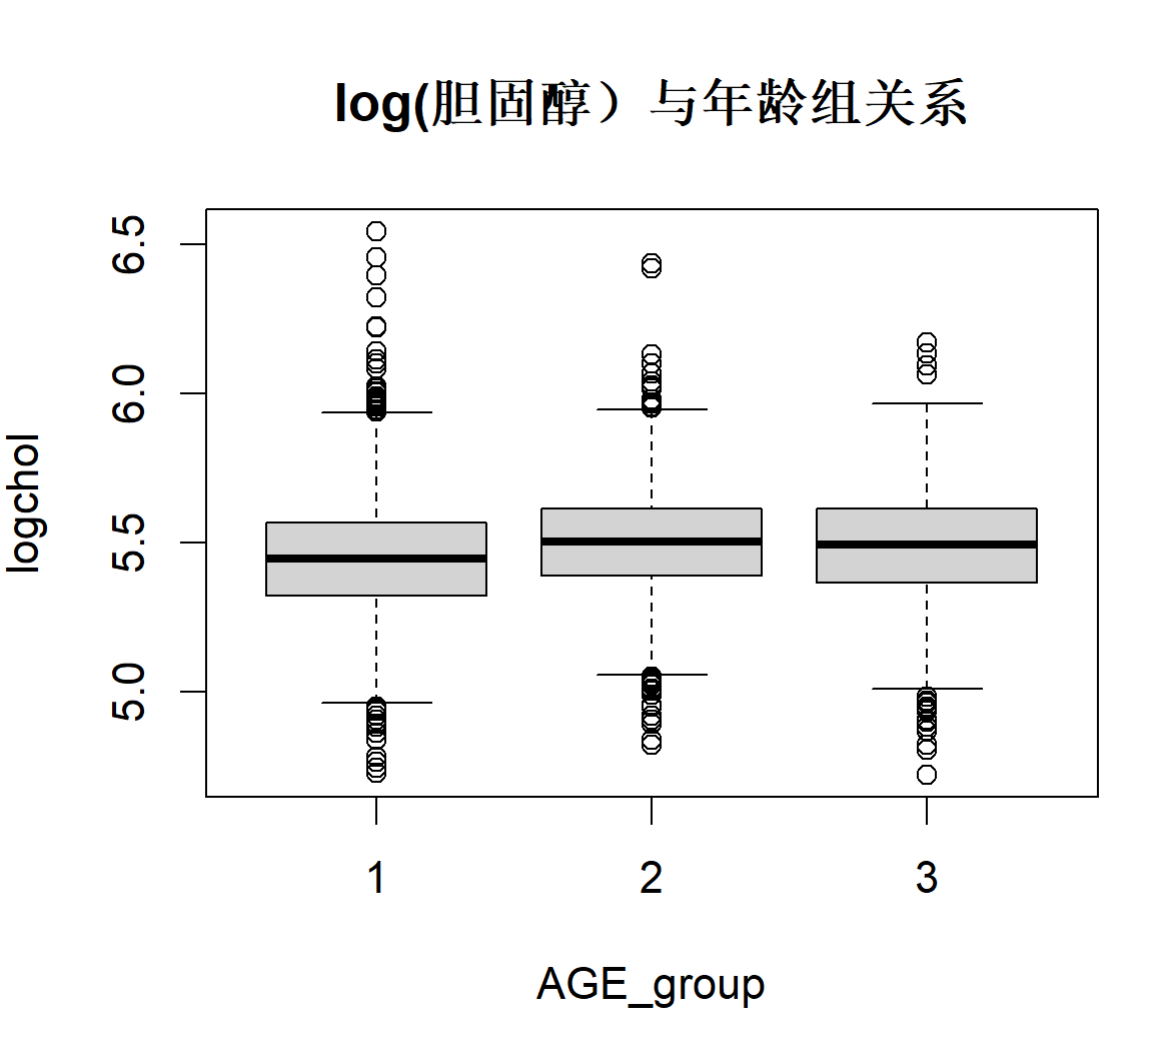
\includegraphics[width=0.7\textwidth]{figs/hw4_age_boxplot.png}
\end{center}

$p\text{-value} < 2 \times 10^{-16}$，拒绝原假设。

\subsubsection*{(ii)}

Plot the residuals to assess the normality and homogeneity of errors.

\textbf{Solution.}

\begin{center}
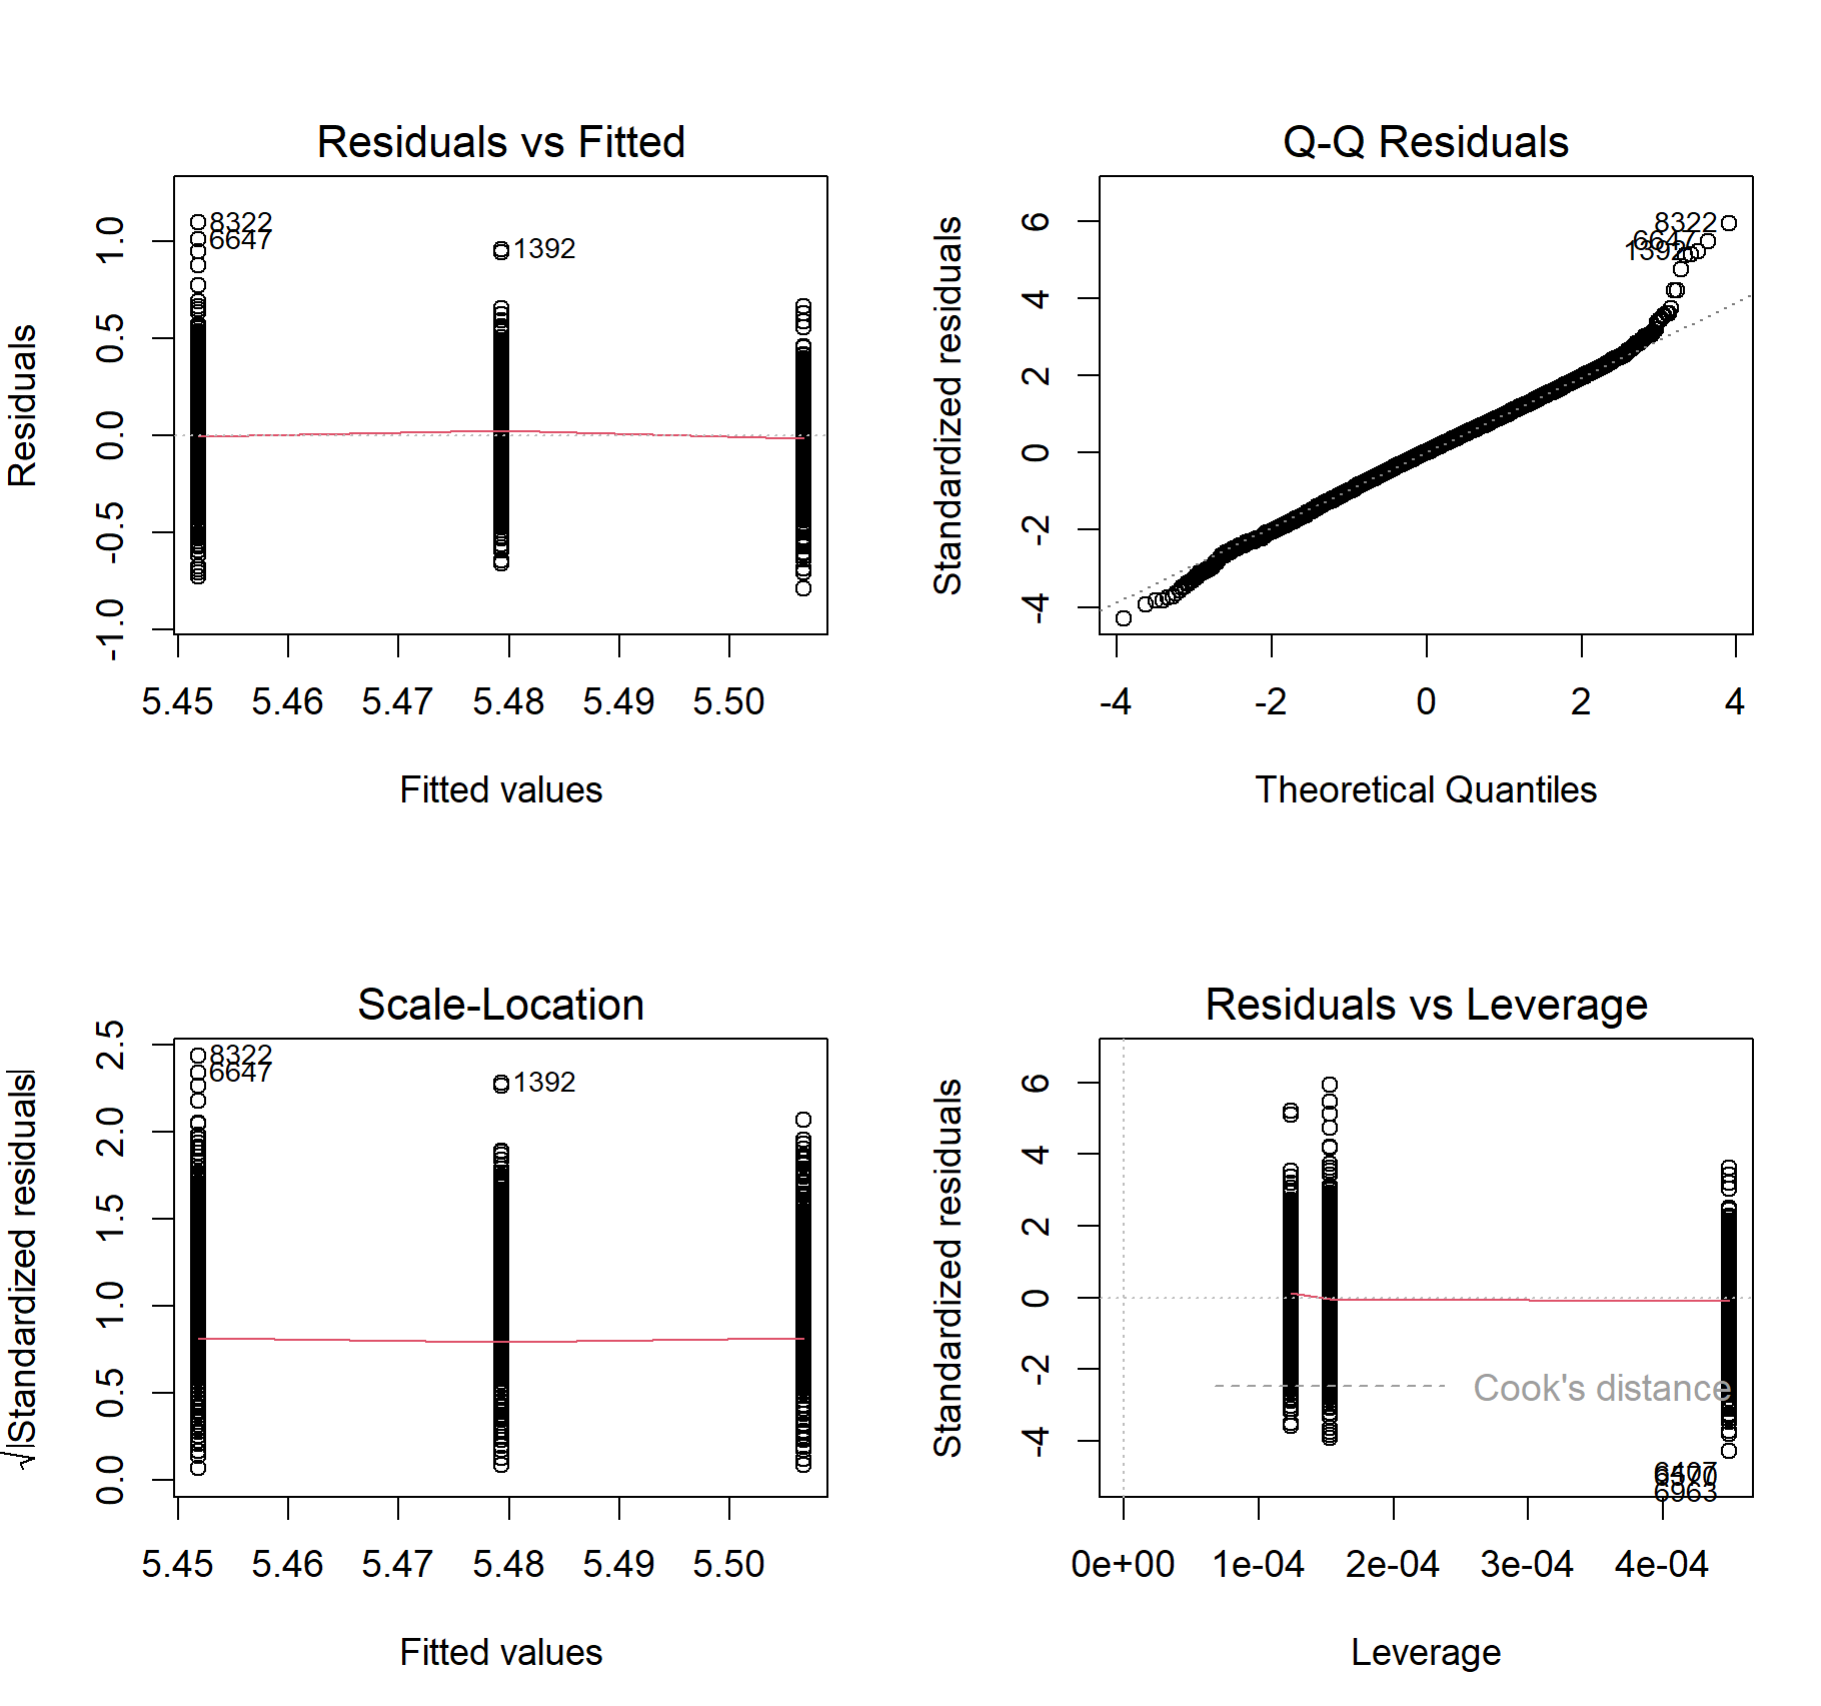
\includegraphics[width=0.8\textwidth]{figs/hw4_age_residuals.png}
\end{center}

\begin{itemize}
    \item normality：大部分点落在斜线上，说明基本服从正态，但发现右尾重尾。
    \item homogeneity：根据 Scale-Location 图，平方根标准化残差拟合线基本水平，虽然有少数离群值但是其整体分布均匀，没有出现明显的异方差情况。
\end{itemize}

综上，使用线性模型是合理的。

\subsubsection*{(iii)}

If the null hypothesis is rejected, perform a post-hoc test.

\textbf{Solution.}

\begin{verbatim}
$AGE_group
           diff         lwr          upr     p adj
2-1  0.05384320  0.04447619  0.063210213 0.0000000
3-1  0.03811704  0.02573994  0.050494134 0.0000000
3-2 -0.01572616 -0.02912186 -0.002330471 0.0163568
\end{verbatim}

如上说明各组之间均有显著关系，且1-2，1-3组间十分显著。

\subsection*{(c)}

Fit an \textbf{ANOVA} model of the outcome on \textbf{sex}.

\subsubsection*{(i)}

Test the null hypothesis of no sex effect. Visualize the data to check their relationship.

\textbf{Solution.}

\begin{center}
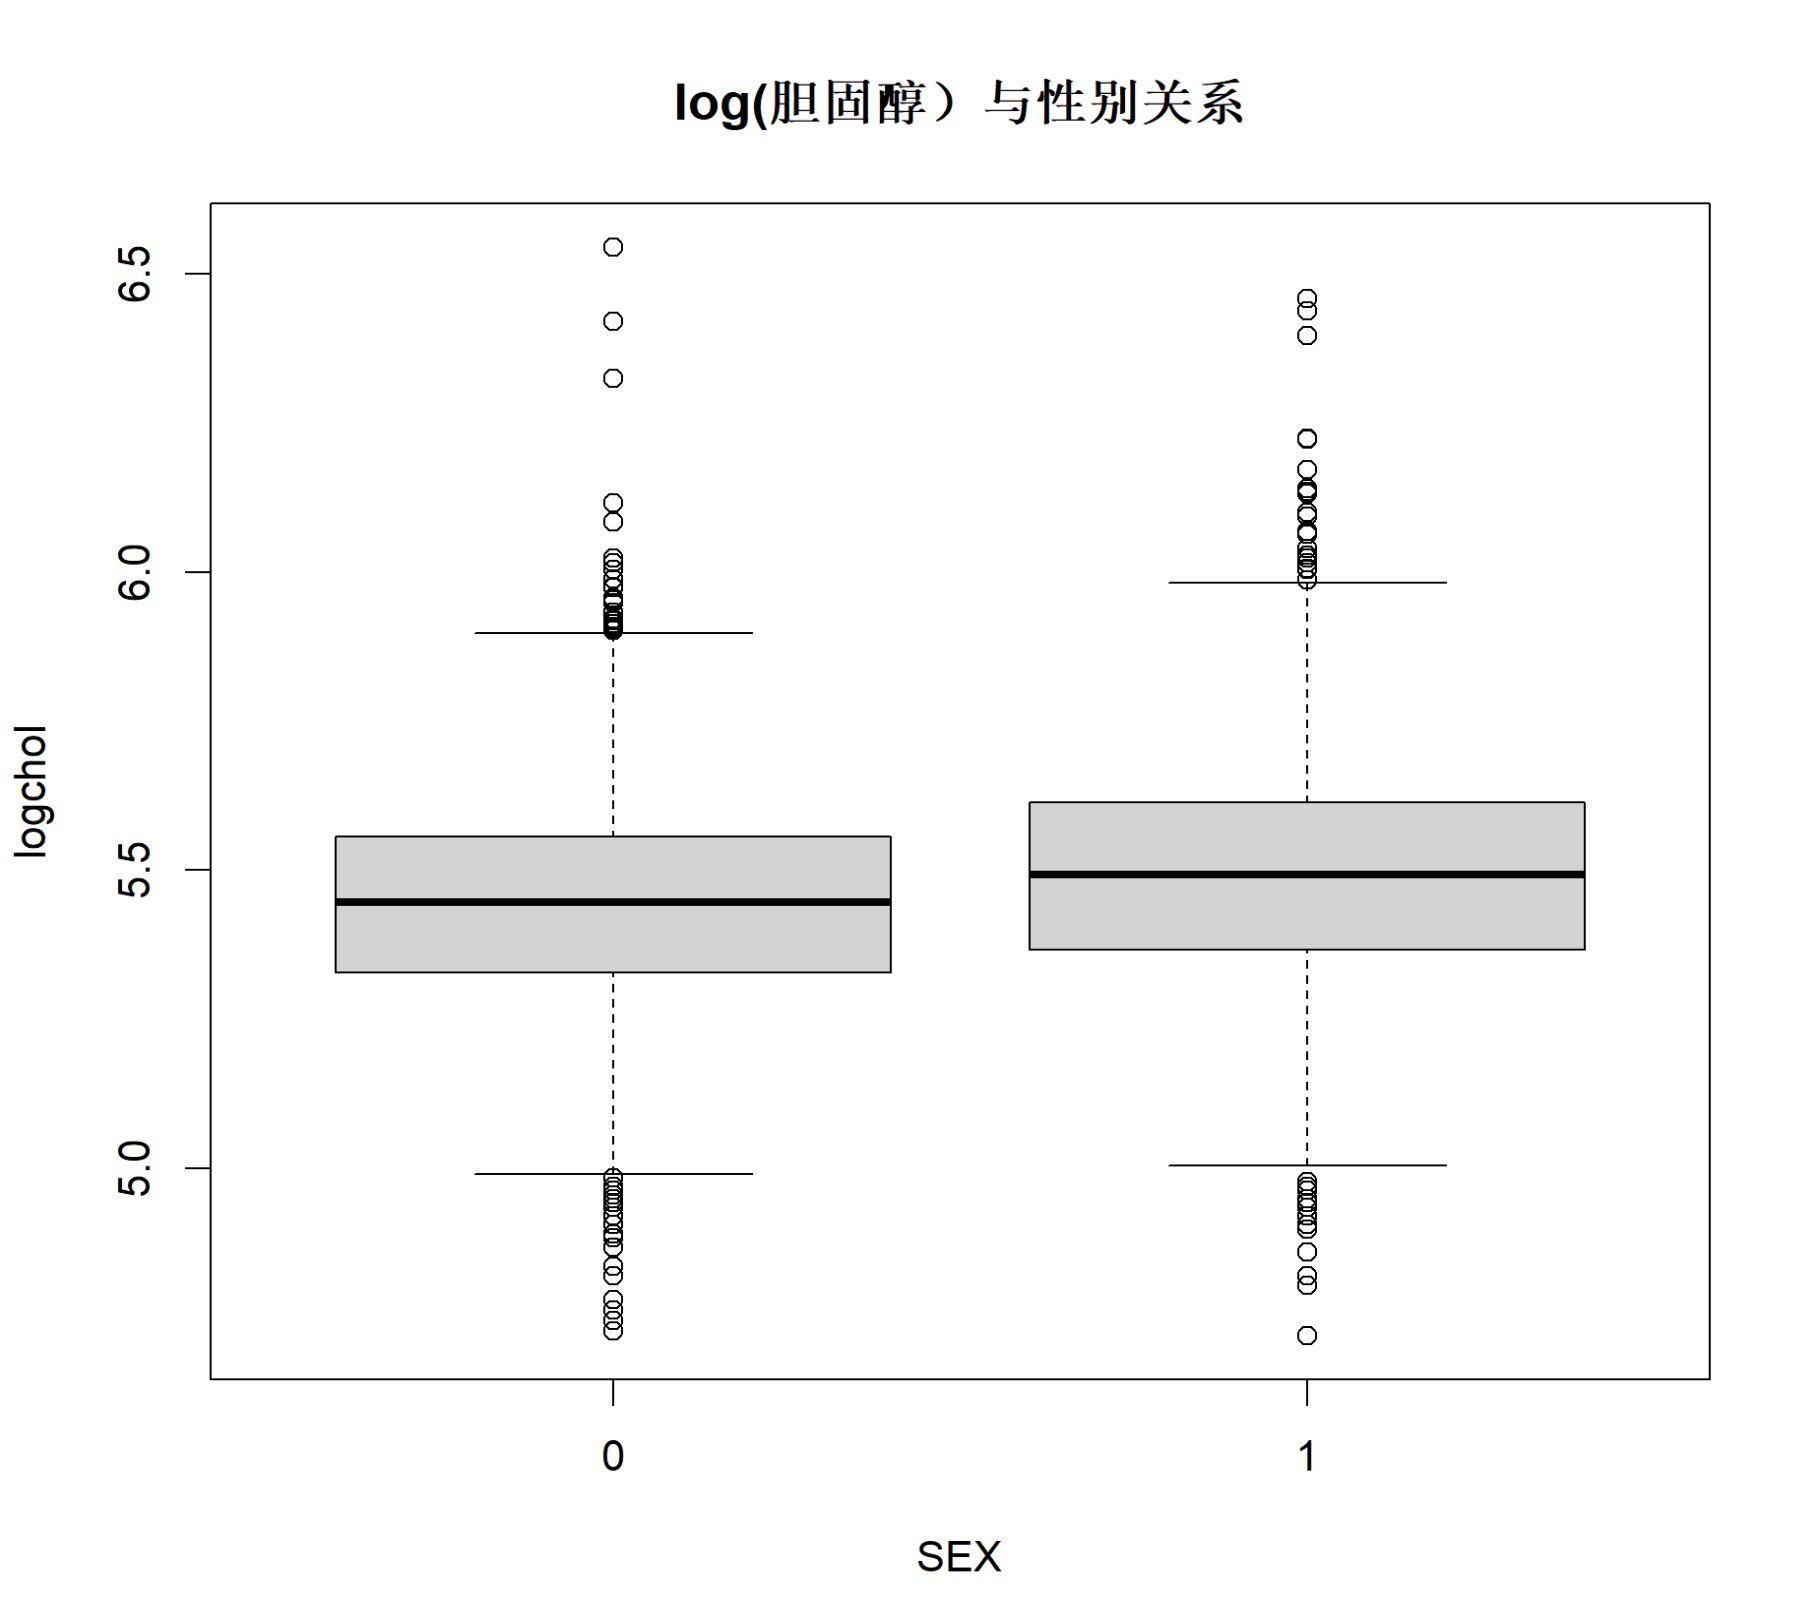
\includegraphics[width=0.7\textwidth]{figs/hw4_sex_boxplot.png}
\end{center}

$p\text{-value} < 2 \times 10^{-16}$，拒绝原假设。

\subsubsection*{(ii)}

Plot the residuals to assess the normality and homogeneity of errors.

\textbf{Solution.}

\begin{center}
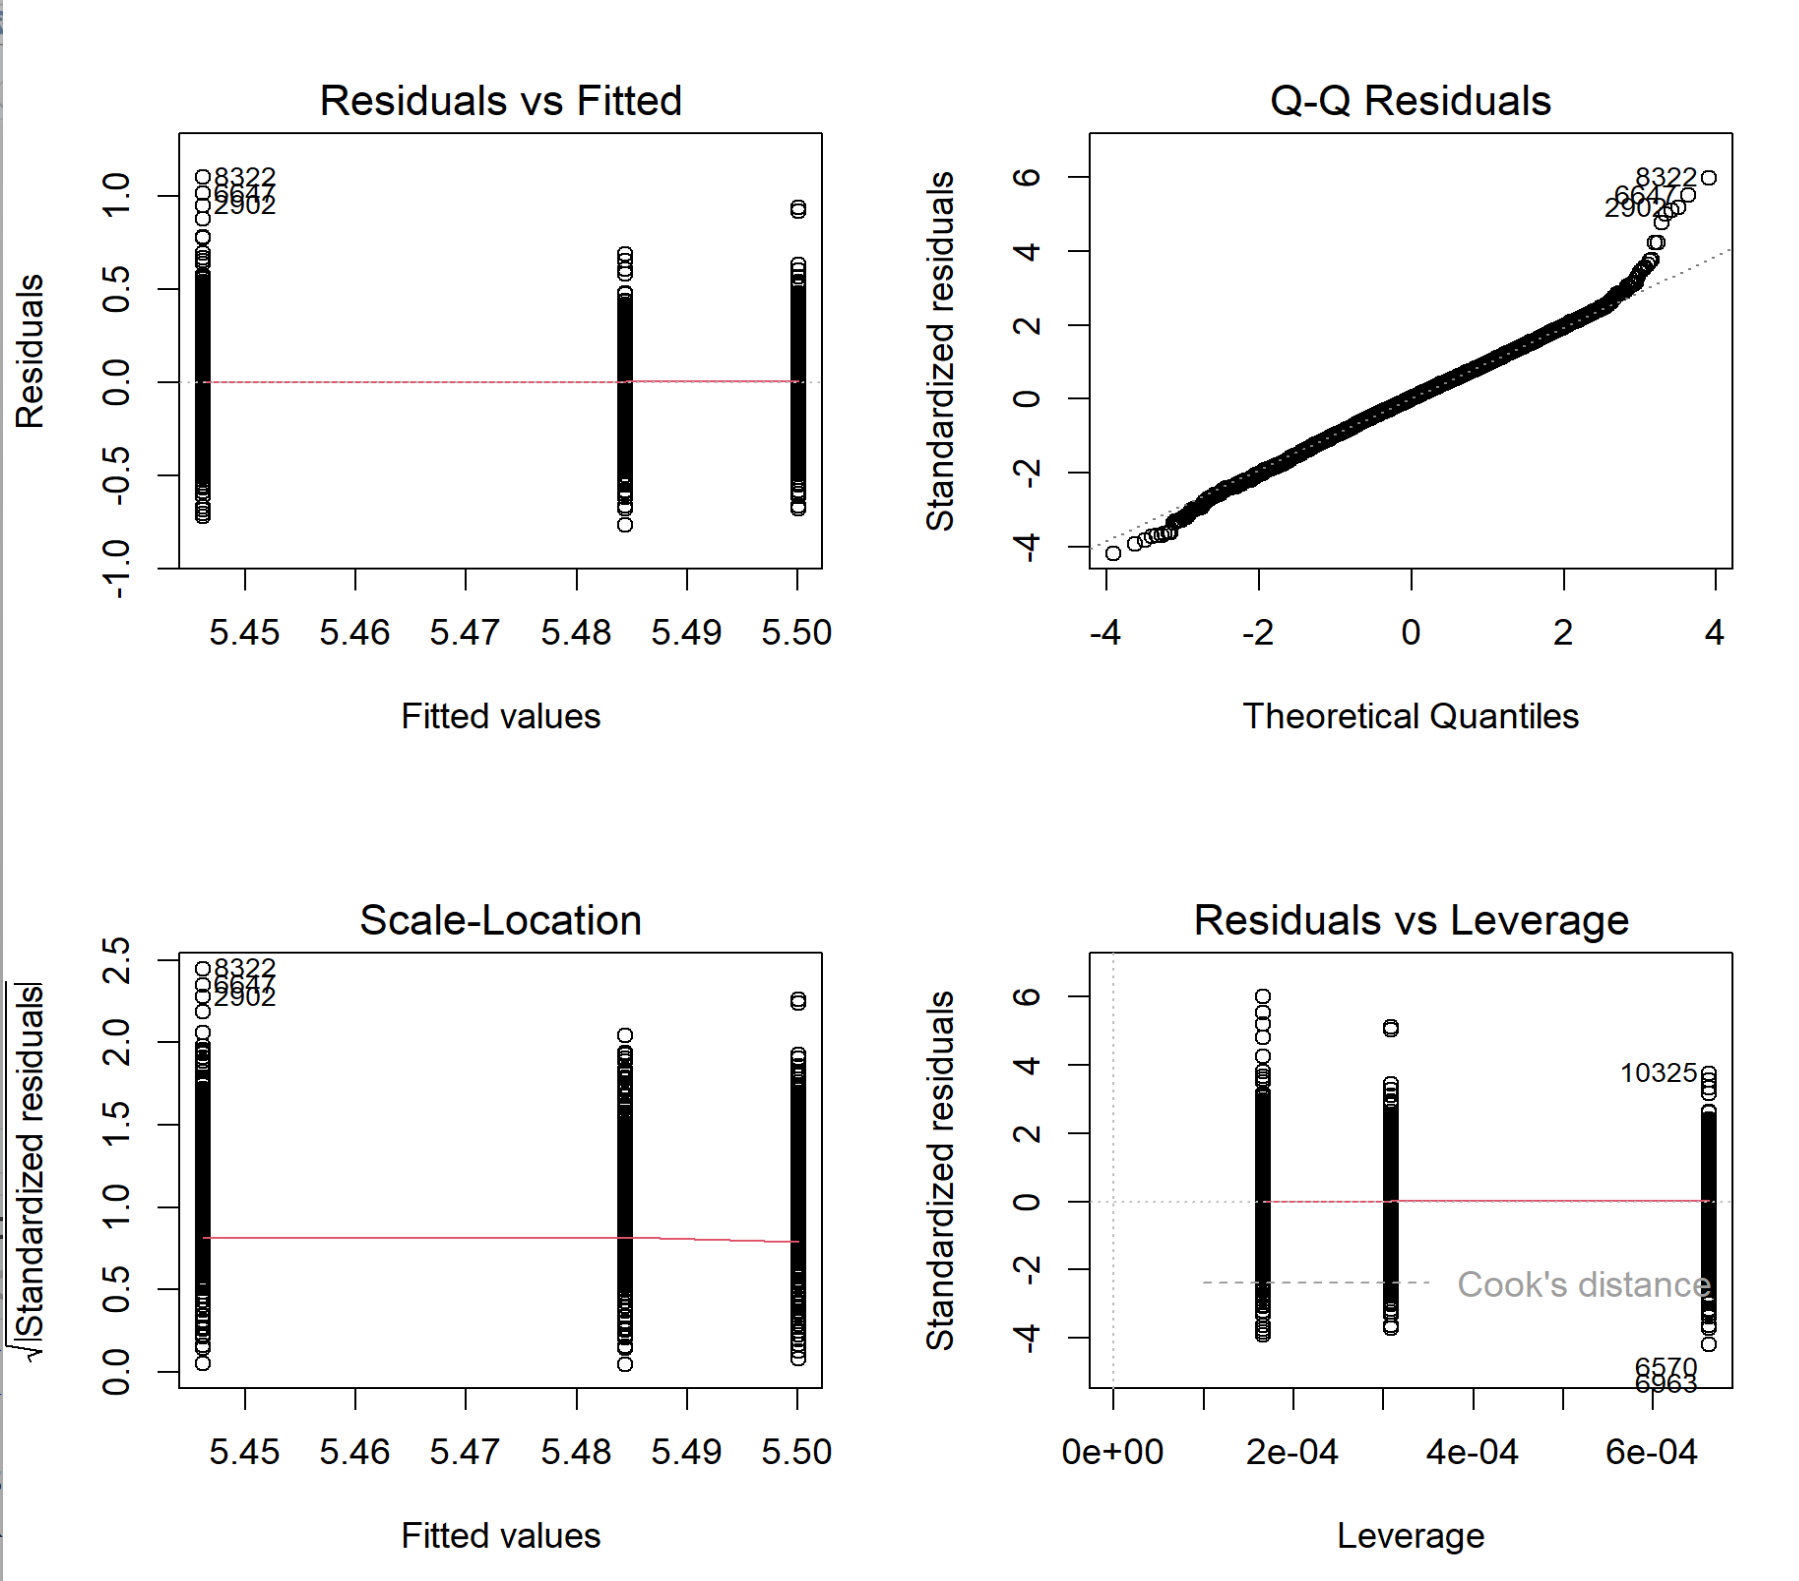
\includegraphics[width=0.8\textwidth]{figs/hw4_sex_residuals.png}
\end{center}

\begin{itemize}
    \item normality：大部分点落在斜线上，说明基本服从正态，但发现右尾重尾。
    \item homogeneity：根据 Scale-Location 图，平方根标准化残差拟合线基本水平，虽然有少数离群值但是其整体分布均匀，没有出现明显的异方差情况。
\end{itemize}

综上，使用线性模型是合理的。

\newpage

%% ===== HW5 =====
\section{Homework 5: Generalized Linear Models 1}
%======================================================================
\subsection{Problem 1}
%======================================================================

\textbf{What are canonical link functions for the following distributions:}

\begin{enumerate}
\item[(a)] $Y$ is an Exponential($\lambda$) random variable with density
\[
f(y;\lambda) = \lambda\exp(-\lambda y) \quad \text{for } y > 0
\]

\textbf{Solution:}

指数族形式：
\[
f(y;\lambda) = \exp\bigl[(-\lambda)\, y + \log\lambda\bigr]
\]

令 $\theta = -\lambda$，则
\[
\mu = E[Y] = \frac{1}{\lambda} = \frac{1}{-\theta} = -\frac{1}{\theta}
\]

Canonical link 满足 $g(\mu) = \theta$，故
\[
\boxed{g(\mu) = \frac{1}{\mu}}
\]

\bigskip

\item[(b)] $Y$ is a Gamma($\mu,\alpha$) random variable with density
\[
f(y;\mu,\alpha) = \frac{1}{\Gamma(\alpha)(\mu/\alpha)^\alpha}\, y^{\alpha-1}\exp(-\alpha y/\mu) \quad \text{for } y > 0
\]

\textbf{Solution:}

将密度写为指数族形式：
\[
f(y;\mu,\alpha) = \exp\!\Bigl[-\frac{\alpha}{\mu}\,y + \alpha\log y - \log\Gamma(\alpha) - \alpha\log\mu + \alpha\log\alpha - \log y\Bigr]
\]

令
\[
\theta = \begin{bmatrix}\theta_1 \\ \theta_2\end{bmatrix} = \begin{bmatrix}-\alpha/\mu \\ \alpha\end{bmatrix}, \qquad T(y) = \begin{bmatrix}y \\ \log y\end{bmatrix}
\]

则 $\mu = -\theta_2/\theta_1$。取 $b(\theta) = \log\Gamma(\theta_2) + \theta_2\log(-\theta_2/\theta_1) - \theta_2\log\theta_2$，可验证
\[
E[Y] = \frac{\partial b(\theta)}{\partial \theta_1} = \mu
\]

故 canonical link 为
\[
\boxed{g(\mu) = \frac{1}{\mu}}
\]

\end{enumerate}

%======================================================================
\subsection{Problem 2}
%======================================================================

\textbf{Consider a Gamma regression model. Let $Y_1,Y_2,\ldots,Y_n$ be independent Gamma($\mu_i,\alpha$) random variables with density}
\[
f(y_i;\mu_i,\alpha) = \frac{1}{\Gamma(\alpha)(\mu_i/\alpha)^\alpha}\, y_i^{\alpha-1}\exp(-\alpha y_i/\mu_i) \quad \text{for } y_i > 0,
\]
\textbf{where $\alpha$ is a fixed known constant (say, $\alpha=1$) and $\mu_i$ is the parameter of interest. Assume that $g(\mu_i) = x_i^T\beta$, $x_i = (x_{i1},x_{i2},\ldots,x_{ip})^T$ and $\beta = (\beta_1,\beta_2,\ldots,\beta_p)^T$.}

\begin{enumerate}
\item[(a)] \textbf{Describe steps to compute the maximum likelihood estimates (MLE) of $\beta$, denoted by $\hat{\beta}$, using Iteratively Reweighted Least Squares (IRLS) for the Gamma regression model.}

\textbf{Solution:}

取 canonical link $g(\mu_i) = 1/\mu_i = x_i^T\beta$（见 Problem 1），则

\begin{itemize}
\item $g'(\mu_i) = -1/\mu_i^2$
\item $\text{Var}(Y_i) = \alpha\cdot\frac{\mu_i^2}{\alpha} = \mu_i^2$（取 $\phi = 1/\alpha$ 为 dispersion 参数）
\item 权重 $W_i = \bigl(V_i\,[g'(\mu_i)]^2\bigr)^{-1} = \frac{\mu_i^4}{\mu_i^2} = \mu_i^2$
\end{itemize}

\textbf{IRLS 算法步骤：}

\begin{enumerate}
\item 选择 $\beta$ 的初始估计 $\hat{\beta}^{(0)}$，代入可得 $\mu_i^{(0)}$，$W_i^{(0)}$

\item 对于第 $k$ 次迭代（$k\in\mathbb{N}_+$）：
  \[
  z_i^{(k)} = g'(\mu_i^{(k)})\bigl(Y_i - \mu_i^{(k)}\bigr) + x_i^T\hat{\beta}^{(k)}
  = \frac{1}{\mu_i^{(k)}} + \frac{1}{(\mu_i^{(k)})^2}\bigl(y_i - \mu_i^{(k)}\bigr)
  \]

\item 更新：
  \[
  \hat{\beta}^{(k+1)} = \bigl(X^T W^{(k)} X\bigr)^{-1} X^T W^{(k)} z^{(k)}
  \]

\item 重复进行直到收敛或达到最大迭代次数，最后得到 $\hat{\beta}$
\end{enumerate}

\bigskip

\item[(b)] \textbf{Derive the variance estimator for $\hat{\beta}$.}

\textbf{Solution:}

最终得到
\[
\text{Var}(\hat{\beta}) = I_n^{-1}(\beta) = \phi\,(X^T W X)^{-1}
\]

即
\[
\boxed{\widehat{\text{Var}}(\hat{\beta}) = \frac{1}{\alpha}\bigl(X^T \hat{W} X\bigr)^{-1}}
\]

\end{enumerate}

%======================================================================
\subsection{Problem 3}
%======================================================================

\textbf{Conduct simulation studies for Gamma Regression models. Simulate the data using the R code provided in class.}

\begin{enumerate}
\item[(a)] \textbf{Fit the Gamma regression model using the IRLS algorithm and estimate the variance of your MLE, both having been derived in Problem 2. Evaluate the performance of your formulas using the following metrics.}

\begin{enumerate}
\item[i.] Compare your $\hat{\beta}_2$ and your variance of $\hat{\beta}_2$ to those obtained from the \texttt{glm(..., family=Gamma(link="inverse"), ...)} function in R.
\item[ii.] Evaluate the bias of $\hat{\beta}_2$.
\item[iii.] Compare the mean of the estimated variance for $\hat{\beta}_2$ and the empirical variance of $\hat{\beta}_2$ based on 10,000 simulations.
\item[iv.] Form the 95\% confidence interval and assess its coverage based on 10,000 simulations.
\end{enumerate}

\textbf{Solution:}

使用 \texttt{link="inverse"}（canonical link）：

\begin{itemize}
\item true $\beta_2 = 0$, $\text{mean}(\hat{\beta}_2) = -0.0006109$
\end{itemize}

\begin{table}[h]
\centering
\begin{tabular}{lr}
\toprule
Evaluation Metric & Value \\
\midrule
bias of $\hat{\beta}_2$ & $-0.0006109$ \\
mean of estimated SE & $0.1096$ \\
mean of estimated variance & $0.01203$ \\
empirical SE & $0.1103$ \\
empirical variance & $0.01217$ \\
average 95\% CI & $[-0.2154,\ 0.2142]$ \\
coverage & $0.9472$ \\
power & $0.0528$ \\
\bottomrule
\end{tabular}
\end{table}

\noindent bias接近0，方差相近，95\%CI覆盖了约95\%的simulation $\beta_2$，power（此处指 type I error）接近0.05，说明 simulation 结果与计算相符。

\bigskip

\item[(b)] \textbf{Examine the impact of mis-specification of the link function: simulate data under the inverse link function and analyze data using the log link. Evaluate the bias, variance, and coverage of 95\% confidence interval as in 3(a) ii--iv.}

\textbf{Solution:}

使用 \texttt{link="log"}（错误的 link function）：

\begin{itemize}
\item true $\beta_2 = 0$, $\text{mean}(\hat{\beta}_2) = 0.0006383$
\end{itemize}

\begin{table}[h]
\centering
\begin{tabular}{lr}
\toprule
Evaluation Metric & Value \\
\midrule
bias of $\hat{\beta}_2$ & $0.0006383$ \\
mean of estimated SE & $0.1095$ \\
mean of estimated variance & $0.01200$ \\
empirical SE & $0.1103$ \\
empirical variance & $0.01217$ \\
average 95\% CI & $[-0.2140,\ 0.2152]$ \\
coverage & $0.9459$ \\
power & $0.0541$ \\
\bottomrule
\end{tabular}
\end{table}

\noindent bias接近0，方差相近，95\%CI覆盖了约95\%的simulation $\beta_2$，power（此处指 type I error）接近0.05，说明虽然使用了错误的 link function 但是 simulation 结果与计算相符。

我尝试给出如下解释：给出的代码中 $\beta_2^{true}=0$，即实际上 $Y$ 与 $X$ 独立，于是两个模型都可拟合。如果我们手动将生成数据的 $\beta$ 进行修改，如令 $\beta_2^{true}=0.05$，\texttt{link="log"}，则 $\text{bias}=-0.09815$，显著变大；$\text{coverage}=0.8534$，与95\%相差较远，$\text{power}=0.07$。这说明模型假设错误。（此时若使用典范链接，coverage仍然接近0.95，二者 power 均约为0.07）

\end{enumerate}

\bigskip

\noindent\textbf{本题所使用的代码：}

\begin{lstlisting}
n.sim = 10000                 # number of simulated replicates of data
n.obs = 1000                   # sample size in each dataset

beta2.true = 0                 # beta for x
# b问中换为0.05, 0.1进行测试
beta.true = c(1, beta2.true)   # beta for (intercept, x)

beta.hat = rep(NA, n.sim)
beta.SEE = rep(NA, n.sim)
beta.var = rep(NA, n.sim)
beta.CI.upper = rep(NA, n.sim)
beta.CI.lower = rep(NA, n.sim)
Wald.stat = rep(NA, n.sim)

set.seed(123)

for (i in 1:n.sim) {

    if (i%%1000 == 0) print(i)

    #--------------------------------
    # simulate data
    #--------------------------------

    x = runif(n=n.obs, min=0, max=1)
    eta = cbind(1, x) %*% beta.true
    mu = 1/eta
    y = rgamma(n=n.obs, shape=1, scale=mu)

    #--------------------------------
    # analyze data
    #--------------------------------

    # (a)
    # res = glm(y~x, family=Gamma(link="inverse"), start=c(1,0))

    # 更换为(b)要求的link
    res = glm(y~x, family=Gamma(link="log"), start=c(1,0))

    #--------------------------------
    # save results for each dataset
    #--------------------------------

    res.coef = coef(summary(res))
    beta.hat[i] = res.coef[2,1]
    beta.SEE[i] = res.coef[2,2]
    beta.var[i] = beta.SEE[i]^2
    beta.CI.upper[i] = res.coef[2,1] + 1.96*res.coef[2,2]
    beta.CI.lower[i] = res.coef[2,1] - 1.96*res.coef[2,2]
    Wald.stat[i] = res.coef[2,1] / res.coef[2,2]
}

#--------------------------------
# summarize results
#--------------------------------

beta2.bias = mean(beta.hat) - beta2.true
beta2.SEE = mean(beta.SEE)
beta2.SE = sd(beta.hat)
beta2.var = var(beta.hat)
mean_var = mean(beta.var)
mean_lower = mean(beta.CI.lower)
mean_upper = mean(beta.CI.upper)
beta2.CR = mean(beta.CI.lower <= beta2.true &
                beta2.true <= beta.CI.upper)
beta2.power = mean(abs(Wald.stat) >= 1.96)

#--------------------------------
# print results
#--------------------------------

print(c(mean(beta.hat), beta2.true))
beta2.var
mean_var
mean_lower
mean_upper
tab = c("bias", "SEE", "SE", "coverage", "power")
tab = rbind(tab, c(beta2.bias, beta2.SEE, beta2.SE,
                    beta2.CR, beta2.power))
tab
\end{lstlisting}

%======================================================================
\subsection{Problem 4}
%======================================================================

\textbf{What are the forms of the Deviance (in terms of $\mu_i$) for the following distributions:}

\begin{enumerate}
\item[(a)] \textbf{Independent variables $Y_1,Y_2,\ldots,Y_n$ follow the inverse Gaussian distribution with the density function}
\[
f(y_i;\mu_i,\sigma) = \frac{1}{\sqrt{2\pi y_i^3\,\sigma^2}}\exp\!\left\{\frac{-(y_i-\mu_i)^2}{2(\mu_i\sigma)^2 y_i}\right\} \quad \text{for } y_i > 0,
\]
\textbf{where $\sigma$ is a fixed constant and $\mu_i$ is the parameter of interest.}

\textbf{Solution:}

\[
D = 2\sum_{i=1}^n\bigl[\tilde{\ell}(y_i) - \hat{\ell}(y_i)\bigr]
\]

其中 $\tilde{\ell}$ 指 Saturated model，有 $\tilde{\mu}_i = y_i$。

log likelihood：
\[
\ell = \exp\!\left[-\frac{(y_i-\mu_i)^2}{2(\mu_i\sigma)^2 y_i} - \frac{1}{2}\log(2\pi y_i^3\sigma^2)\right], \quad \sigma \text{ 已知}
\]

\[
\boxed{D = 2\sum_{i=1}^n \frac{(y_i - \hat{\mu}_i)^2}{2(\hat{\mu}_i\,\sigma)^2\,y_i} = \frac{1}{\sigma^2}\sum_{i=1}^n \frac{(y_i - \hat{\mu}_i)^2}{\hat{\mu}_i^2\,y_i}}
\]

\bigskip

\item[(b)] \textbf{Independent variables $Y_1,Y_2,\ldots,Y_n$ follow the Gamma($\mu_i,\alpha$) distribution with the density function}
\[
f(y_i;\mu_i,\alpha) = \frac{1}{\Gamma(\alpha)(\mu_i/\alpha)^\alpha}\, y_i^{\alpha-1}\exp(-\alpha y_i/\mu_i) \quad \text{for } y_i > 0,
\]
\textbf{where $\alpha$ is a fixed constant and $\mu_i$ is the parameter of interest.}

\textbf{Solution:}

log likelihood：
\[
\ell = -\alpha\frac{y_i}{\mu_i} - (\alpha-1)\log y_i - \log\Gamma(\alpha) - \alpha\log\frac{\mu_i}{\alpha}
\]

\[
D = 2\sum_{i=1}^n\left[-\alpha\!\left(1 - \frac{y_i}{\hat{\mu}_i}\right) - \alpha\log\frac{y_i}{\hat{\mu}_i}\right]
\]

\[
\boxed{D = 2\alpha\sum_{i=1}^n\left[\frac{y_i}{\hat{\mu}_i} - 1 + \log\frac{\hat{\mu}_i}{y_i}\right]}
\]

\end{enumerate}

\newpage

%% ===== HW6 =====
\section{Homework 6: Generalized Linear Models 2}
%======================================================================
\subsection{Problem 1}
%======================================================================

\textbf{Consider $Y \mid \pi \sim \text{Binomial}(n, \pi)$, where $\pi \sim \text{Beta}(\alpha, \beta)$. Find $\text{Var}(Y)$.}

\textbf{Solution:}

由方差分解公式：
\[
\text{Var}(Y) = \text{Var}[E(Y \mid \pi)] + E[\text{Var}(Y \mid \pi)]
\]

由于 $Y \mid \pi \sim \text{Binomial}(n, \pi)$，有：
\[
E(Y \mid \pi) = n\pi, \quad \text{Var}(Y \mid \pi) = n\pi(1-\pi)
\]

代入得：
\[
\text{Var}(Y) = \text{Var}(n\pi) + E[n\pi(1-\pi)]
\]

而 $\pi \sim \text{Beta}(\alpha, \beta)$ 的性质为：
\[
E(\pi) = \frac{\alpha}{\alpha+\beta}, \quad \text{Var}(\pi) = \frac{\alpha\beta}{(\alpha+\beta)^2(\alpha+\beta+1)}
\]

计算 $E[\pi(1-\pi)]$：
\begin{align*}
E[\pi(1-\pi)] &= E\pi - E\pi^2 \\
&= \frac{\alpha}{\alpha+\beta} - \left(\frac{\alpha\beta}{(\alpha+\beta)^2(\alpha+\beta+1)} + \frac{\alpha^2}{(\alpha+\beta)^2}\right) \\
&= \frac{\alpha(\alpha+\beta)(\alpha+\beta+1) - \alpha\beta - \alpha^2(\alpha+\beta+1)}{(\alpha+\beta)^2(\alpha+\beta+1)} \\
&= \frac{\alpha^2\beta + \alpha\beta^2}{(\alpha+\beta)^2(\alpha+\beta+1)} = \frac{\alpha\beta}{(\alpha+\beta)(\alpha+\beta+1)}
\end{align*}

因此：
\begin{align*}
\text{Var}(Y) &= \frac{n^2\alpha\beta}{(\alpha+\beta)^2(\alpha+\beta+1)} + \frac{n\alpha\beta}{(\alpha+\beta)(\alpha+\beta+1)} \\
&= \boxed{\frac{n\alpha\beta(n+\alpha+\beta)}{(\alpha+\beta)^2(\alpha+\beta+1)}}
\end{align*}

\textbf{Remark:} 此处也可看出 $\text{Var}(Y)$ 有 over-dispersion（因为 $\text{Var}(Y) > n\mu(1-\mu)$，其中 $\mu = \frac{\alpha}{\alpha+\beta}$）。

%======================================================================
\subsection{Problem 2}
%======================================================================

\textbf{Consider the quasi-likelihood function}
\[
Q_i(\mu_i; y_i) = \int_{y_i}^{\mu_i} \frac{y_i - t}{V^*(t)} \, dt
\]
\textbf{where $V^*(\mu_i) = \text{Var}(Y_i) / \phi$ is the variance function. Show that:}

\begin{enumerate}
\item[(a)] $\frac{\partial Q_i}{\partial \mu_i} = \frac{y_i - \mu_i}{V^*(\mu_i)}$

\textbf{Solution:}

由积分上限函数求导公式：
\[
\frac{\partial Q_i}{\partial \mu_i} = \frac{y_i - \mu_i}{V^*(\mu_i)}
\]

取期望：
\[
E\left(\frac{\partial Q_i}{\partial \mu_i}\right) = \frac{E(Y_i) - \mu_i}{V^*(\mu_i)} = \frac{\mu_i - \mu_i}{V^*(\mu_i)} = 0
\]

\bigskip

\item[(b)] $\frac{\partial Q_i}{\partial \beta_j} = \sum_{i=1}^{n} \frac{\partial Q_i}{\partial \mu_i} \cdot \frac{\partial \mu_i}{\partial \beta_j}$

\textbf{Solution:}

由链式法则：
\[
\frac{\partial Q_i}{\partial \beta_j} = \frac{\partial Q_i}{\partial \mu_i} \cdot \frac{\partial \mu_i}{\partial \beta_j}
\]

取期望，由(a)知 $E\left(\frac{\partial Q_i}{\partial \mu_i}\right) = 0$，故：
\[
E\left(\frac{\partial Q_i}{\partial \beta_j}\right) = 0
\]

\bigskip

\item[(c)] $\frac{\partial^2 Q_i}{(\partial \mu_i)^2} = \frac{-1}{V^*(\mu_i)} - \frac{(y_i - \mu_i) \cdot \frac{dV^*(\mu_i)}{d\mu_i}}{[V^*(\mu_i)]^2}$

\textbf{Solution:}

对(a)中的结果关于 $\mu_i$ 求导：
\begin{align*}
\frac{\partial^2 Q_i}{(\partial \mu_i)^2} &= \frac{\partial}{\partial \mu_i}\left(\frac{y_i - \mu_i}{V^*(\mu_i)}\right) \\
&= \frac{-V^*(\mu_i) - (y_i - \mu_i) \cdot \frac{dV^*(\mu_i)}{d\mu_i}}{[V^*(\mu_i)]^2} \\
&= \frac{-1}{V^*(\mu_i)} - \frac{(y_i - \mu_i) \cdot \frac{dV^*(\mu_i)}{d\mu_i}}{[V^*(\mu_i)]^2}
\end{align*}

后一项对 $Y_i$ 取期望得到 0（因为 $E(y_i - \mu_i) = 0$），故：
\[
E\left(\frac{\partial^2 Q_i}{(\partial \mu_i)^2}\right) = \frac{-1}{V^*(\mu_i)}
\]

\bigskip

\item[(d)] $E\left[\frac{\partial^2 Q_i}{\partial \beta_j \partial \beta_k}\right] = E\left[\frac{\partial Q_i}{\partial \mu_i}\right]^2 \cdot \frac{\partial \mu_i}{\partial \beta_j} \cdot \frac{\partial \mu_i}{\partial \beta_k}$

\textbf{Solution:}

\begin{align*}
\frac{\partial}{\partial \beta_j}\left(\frac{\partial Q_i}{\partial \beta_k}\right) &= \frac{\partial}{\partial \beta_j}\left(\frac{\partial Q_i}{\partial \mu_i} \cdot \frac{\partial \mu_i}{\partial \beta_k}\right) \\
&= \left(\frac{\partial^2 Q_i}{\partial \mu_i^2} \cdot \frac{\partial \mu_i}{\partial \beta_k} + \frac{\partial Q_i}{\partial \mu_i} \cdot \frac{\partial^2 \mu_i}{\partial \mu_i \partial \beta_k}\right) \cdot \frac{\partial \mu_i}{\partial \beta_j}
\end{align*}

取期望，由(c)知 $E\left(\frac{\partial^2 Q_i}{\partial \mu_i^2}\right) = \frac{-1}{V^*(\mu_i)}$，且 $E\left(\frac{\partial Q_i}{\partial \mu_i}\right) = 0$，故：
\[
E \frac{\partial}{\partial \beta_j}\left(\frac{\partial Q_i}{\partial \beta_k}\right) = E\left(\frac{\partial^2 Q_i}{\partial \mu_i^2}\right) \cdot \frac{\partial \mu_i}{\partial \beta_k} \cdot \frac{\partial \mu_i}{\partial \beta_j}
\]

又有：
\[
E\left[\frac{\partial Q_i}{\partial \beta_j} \cdot \frac{\partial Q_i}{\partial \beta_k}\right] = E\left(\frac{\partial Q_i}{\partial \mu_i}\right)^2 \cdot \frac{\partial \mu_i}{\partial \beta_j} \cdot \frac{\partial \mu_i}{\partial \beta_k}
\]

则由(c)即得结论。
\end{enumerate}

%======================================================================
\subsection{Problem 3}
%======================================================================

\textbf{Let $Y_1, Y_2, \ldots, Y_n$ be binary random variables with $P(Y_i = 1) = \pi$, $P(Y_i = 0) = 1 - \pi$. Let $Y = \sum_{i=1}^n Y_i$.}

\begin{enumerate}
\item[(a)] \textbf{Suppose $Y_1, Y_2, \ldots, Y_n$ are independent. Find $\text{Var}(Y)$.}

\textbf{Solution:}

Variance of Binomial: $\text{Var} = n\pi(1-\pi)$

对于(a)中情景：
\begin{align*}
\widetilde{\text{Var}} &= E(Y - \bar{Y})^2 = \pi(n - n\pi)^2 + (1-\pi)(n\pi)^2 \\
&= n^2\pi - 2n^2\pi^2 + n^2\pi^3 + n^2\pi^2 - n^2\pi^3 \\
&= n^2\pi(1-\pi)
\end{align*}

$n > 1$ 时有 $\widetilde{\text{Var}} > \text{Var}$，体现了 Overdispersion！

\bigskip

\item[(b)] \textbf{Now suppose $\text{Cov}(Y_i, Y_j) = \rho \pi(1-\pi)$ for all $i \neq j$. Find $\text{Var}(Y)$.}

\textbf{Solution:}

（注意到(a)即为 $\rho = 1$ 情形）

$\rho = 0$ 时：
\begin{align*}
\text{Var}_{\rho} &= \sum_i \text{Var}(Y_i) + \sum_{i \neq j} \text{Cov}(Y_i, Y_j) \\
&= n\pi(1-\pi) + n(n-1)\pi(1-\pi)\rho > \text{Var} = n\pi(1-\pi)
\end{align*}

\bigskip

\item[(c)] \textbf{If $\rho = -1$, what is $\text{Var}(Y)$?}

\textbf{Solution:}

由于 $n$ even，故 $Y \equiv \frac{n}{2}$

$\{Y_i\}$ 形如 $\{1, 0, 1, 0, \ldots, 1, 0\}$ 或 $\{0, 1, 0, 1, \ldots, 0, 1\}$

故 $\text{Var}_{-1} = 0 < \text{Var}$，($0 < \pi < 1$)
\end{enumerate}

%======================================================================
\subsection{Problem 4}
%======================================================================

\textbf{Use the Framingham data to fit a logistic regression model with TOTCHOL as the response (grouped by AGE\_group) and AGE\_group as the predictor.}

\textbf{Solution:}

缺失数据处理方式：仅保留了本题所用的 AGE\_group 和 TOTCHOL 均存在的数据，删除了缺失数据。

\begin{lstlisting}[caption={Data Preparation}]
df <- read.csv("Framingham_data.csv")
dfclean <- df[complete.cases(df[, c("AGE_group", "TOTCHOL")]), ]
dfclean$bi_chole <- ifelse(dfclean$TOTCHOL > 200, 1, 0)
\end{lstlisting}

\begin{enumerate}
\item[(a)] \textbf{Fit the model using both ungrouped and grouped data. Report the deviance for each.}

\textbf{Solution:}

\begin{lstlisting}[caption={Ungrouped Data Analysis}]
# ungrouped data
model_ungrouped <- glm(bi_chole ~ AGE_group,
                       data = dfclean,
                       family = binomial(link = "logit"))
summary(model_ungrouped)
\end{lstlisting}

Ungrouped 结果：
\begin{verbatim}
    Null deviance: 10221  on 10767  degrees of freedom
Residual deviance: 10164  on 10766  degrees of freedom
\end{verbatim}

\begin{lstlisting}[caption={Grouped Data Analysis}]
# grouped data
library(dplyr)

grouped <- dfclean %>%
  group_by(AGE_group) %>%
  summarise(
    ynum = sum(bi_chole),   # 高胆固醇人数
    n = n()                 # 总人数
  ) %>%
  ungroup()

model_grouped <- glm(cbind(ynum, (n - ynum)) ~ AGE_group,
                     data = grouped,
                     family = binomial(link = "logit"))
summary(model_grouped)
\end{lstlisting}

Grouped 结果：
\begin{verbatim}
    Null deviance: 102.924  on 2  degrees of freedom
Residual deviance:  46.479  on 1  degrees of freedom
\end{verbatim}

注意到两组数据均有 $M_0 > M_1$，且 $D_0 - D_1$ 分别为 57 和约 56.4，说明无论使用哪种方法，均认为 AGE\_group 均对胆固醇（二分值）有显著影响。

又发现 ungrouped 的 deviance 远大于 grouped。这是因为在 glm 中，$D = 2(l_{\text{saturated}} - l_{\text{model}})$ 而两种数据形式对应的饱和模型不同。ungrouped 的饱和模型对应每个观测单独拟合，因此对数似然差值很大；而 grouped 的饱和模型只需要拟合 $\hat{p}_j = \frac{y_j}{n_j}$，对数似然差值远小于前者。

\bigskip

\item[(b)] \textbf{Compare the deviance differences $D_0 - D_1$ from both analyses. Are they the same? Why?}

\textbf{Solution:}

在(a)中已经得到两者的 deviance 差值相近。

理论上二者应该完全相等，因为：
\[
D_0 - D_1 = 2(l_{\text{saturated}} - l_{M_0}) - 2(l_{\text{saturated}} - l_{M_1}) = -2(l_{M_0} - l_{M_1})
\]

即此处 deviance 的差不依赖于数据表示方式。

如果我们使用手动计算 deviance 的方式来进行，可以得到差值均为 56.44513，验证了相等性。直接使用 glm 函数得出 0.6 左右的差值可能是因为计算过程累计误差等因素导致的。

\begin{lstlisting}[caption={Manual Deviance Calculation}]
# ungrouped
model0_ung <- glm(bi_chole ~ 1,
                  data = dfclean,
                  family = binomial(link = "logit"))
model1_ung <- glm(bi_chole ~ AGE_group,
                  data = dfclean,
                  family = binomial(link = "logit"))
delta_def_ung <- 2 * (logLik(model1_ung) - logLik(model0_ung))

# grouped
model0_grp <- glm(cbind(ynum, n - ynum) ~ 1,
                  data = grouped,
                  family = binomial(link = "logit"))
model1_grp <- glm(cbind(ynum, n - ynum) ~ AGE_group,
                  data = grouped,
                  family = binomial(link = "logit"))
delta_def_grp <- 2 * (logLik(model1_grp) - logLik(model0_grp))

# output
delta_def_ung
delta_def_grp
\end{lstlisting}
\end{enumerate}

\newpage

%% ===== HW7 =====
\section{Homework 7: Longitudinal Data Analysis}
%% ==================== Problem 1 ====================
\subsection{Problem 1}

\textbf{Question:} Show that the loglinear random effects model
\[
  \log[E(Y_{it}\mid \boldsymbol{b}_i)] = \boldsymbol{x}_{it}'\boldsymbol{\beta} + \boldsymbol{z}_{it}'\boldsymbol{b}_i,
\]
where $\{\boldsymbol{b}_i\}$ are independent $N(\boldsymbol{0}, \boldsymbol{\Sigma})$, implies the marginal loglinear model
\[
  \log[E(Y_{it})] = \boldsymbol{x}_{it}'\boldsymbol{\beta} + \frac{1}{2}\boldsymbol{z}_{it}'\boldsymbol{\Sigma}\boldsymbol{z}_{it},
\]
with the same fixed effects but with offset term. Explain why $\frac{1}{2}\boldsymbol{z}_{it}'\boldsymbol{\Sigma}\boldsymbol{z}_{it}$ is an offset term.

(Hint: use the moment generating function for a normal variable $\boldsymbol{b} \sim N(\boldsymbol{\mu}, \boldsymbol{\Sigma})$: $E(\exp(\boldsymbol{t}'\boldsymbol{b})) = \exp(\boldsymbol{t}'\boldsymbol{\mu} + \frac{1}{2}\boldsymbol{t}'\boldsymbol{\Sigma}\boldsymbol{t})$)

\bigskip
\textbf{Solution:}

由条件期望的定义：
\[
  E(Y_{it}\mid \boldsymbol{b}_i) = \exp(\boldsymbol{x}_{it}'\boldsymbol{\beta} + \boldsymbol{z}_{it}'\boldsymbol{b}_i).
\]

对随机效应 $\boldsymbol{b}_i$ 取期望，得边际期望：
\begin{align*}
  E(Y_{it}) &= E_{\boldsymbol{b}_i}\big[E(Y_{it}\mid \boldsymbol{b}_i)\big] \\
  &= E_{\boldsymbol{b}_i}\big[\exp(\boldsymbol{x}_{it}'\boldsymbol{\beta} + \boldsymbol{z}_{it}'\boldsymbol{b}_i)\big] \\
  &= \exp(\boldsymbol{x}_{it}'\boldsymbol{\beta}) \cdot E\big[\exp(\boldsymbol{z}_{it}'\boldsymbol{b}_i)\big].
\end{align*}

由于 $\boldsymbol{b}_i \sim N(\boldsymbol{0}, \boldsymbol{\Sigma})$，利用正态分布的矩生成函数（MGF），取 $\boldsymbol{t} = \boldsymbol{z}_{it}$，$\boldsymbol{\mu} = \boldsymbol{0}$：
\[
  E\big[\exp(\boldsymbol{z}_{it}'\boldsymbol{b}_i)\big] = \exp\!\Big(\boldsymbol{0}'\boldsymbol{z}_{it} + \frac{1}{2}\boldsymbol{z}_{it}'\boldsymbol{\Sigma}\boldsymbol{z}_{it}\Big) = \exp\!\Big(\frac{1}{2}\boldsymbol{z}_{it}'\boldsymbol{\Sigma}\boldsymbol{z}_{it}\Big).
\]

因此：
\[
  E(Y_{it}) = \exp(\boldsymbol{x}_{it}'\boldsymbol{\beta}) \cdot \exp\!\Big(\frac{1}{2}\boldsymbol{z}_{it}'\boldsymbol{\Sigma}\boldsymbol{z}_{it}\Big) = \exp\!\Big(\boldsymbol{x}_{it}'\boldsymbol{\beta} + \frac{1}{2}\boldsymbol{z}_{it}'\boldsymbol{\Sigma}\boldsymbol{z}_{it}\Big).
\]

取对数得边际对数线性模型：
\[
  \log[E(Y_{it})] = \boldsymbol{x}_{it}'\boldsymbol{\beta} + \frac{1}{2}\boldsymbol{z}_{it}'\boldsymbol{\Sigma}\boldsymbol{z}_{it}.
\]

\textbf{关于 offset term 的解释：} offset term（偏移项）是在模型中不参与参数估计的已知项，其系数固定为1。此处 $\frac{1}{2}\boldsymbol{z}_{it}'\boldsymbol{\Sigma}\boldsymbol{z}_{it}$ 由已知的协变量 $\boldsymbol{z}_{it}$ 和已知的协方差矩阵 $\boldsymbol{\Sigma}$ 构成，不需要进行估计，因此是 offset term。另外，由于 $\exp$ 变换不是线性的，因此需要进行均值的修正。


%% ==================== Problem 2 ====================
\subsection{Problem 2}

\textbf{Question:} Let $\boldsymbol{Y}_1, \ldots, \boldsymbol{Y}_n$ be independent random vectors, where $\boldsymbol{Y}_i = (Y_{i1}, Y_{i2})^T$ are two repeated measurements from subject $i$. Assume that
\[
  E(Y_{ij}) = \mu_{ij} = \beta_0 + x_i\beta_1, \quad \text{Var}(Y_{ij}) = \sigma^2, \quad i=1,\ldots,n,\; j=1,2
\]
where the subject-level covariates $x_i$ are iid variables and the variance $\sigma^2$ are known. Also assume that $\text{corr}(Y_{i1}, Y_{i2}) = \alpha$, where $\alpha > 0$ is known.

\begin{enumerate}[label=(\alph*)]
  \item Write down the matrices $V_i = \text{Var}(\boldsymbol{Y}_i)$ and
  \[
    D_i = \begin{pmatrix} \frac{\partial \mu_{i1}}{\partial \beta_0} & \frac{\partial \mu_{i1}}{\partial \beta_1} \\[4pt] \frac{\partial \mu_{i2}}{\partial \beta_0} & \frac{\partial \mu_{i2}}{\partial \beta_1} \end{pmatrix}.
  \]
  Calculate the following terms: $D_i^T V_i^{-1} D_i$, $D_i^T D_i$, and $D_i^T V_i D_i$.

  \item Let $\widehat{\boldsymbol{\beta}}_E = (\widehat{\beta}_{0E}, \widehat{\beta}_{1E})$ denote the estimate of $\boldsymbol{\beta}$ under a GEE model with an exchangeable correlation structure, and $\widehat{\boldsymbol{\beta}}_I = (\widehat{\beta}_{0I}, \widehat{\beta}_{1I})$ denote the estimate of $\boldsymbol{\beta}$ under a GEE model with an independent correlation structure. Show their asymptotic variances (avar) to be
  \[
    n\,\text{avar}(\widehat{\boldsymbol{\beta}}_E) = \bigg(\lim_{n\to\infty} \frac{1}{n}\sum_{i=1}^n D_i^T V_i^{-1} D_i\bigg)^{-1}
  \]
  \[
    n\,\text{avar}(\widehat{\boldsymbol{\beta}}_I) = \bigg(\lim_{n\to\infty}\frac{1}{n}\sum_{i=1}^n D_i^T D_i\bigg)^{-1} \bigg(\lim_{n\to\infty}\frac{1}{n}\sum_{i=1}^n D_i^T V_i D_i\bigg) \bigg(\lim_{n\to\infty}\frac{1}{n}\sum_{i=1}^n D_i^T D_i\bigg)^{-1}
  \]

  \item Evaluate the asymptotic relative efficiency of $\widehat{\beta}_{1E}$ (the slope estimator) versus $\widehat{\beta}_{1I}$:
  \[
    \lim_{n\to\infty} \frac{n\,\text{avar}(\widehat{\beta}_{1E})}{n\,\text{avar}(\widehat{\beta}_{1I})}.
  \]
\end{enumerate}

\bigskip
\textbf{Solution:}

\begin{enumerate}[label=(\alph*)]
\item 由题意，$\mu_{ij} = \beta_0 + x_i\beta_1$，因此
\[
  D_i = \begin{pmatrix} 1 & x_i \\ 1 & x_i \end{pmatrix}.
\]

协方差矩阵为
\[
  V_i = \text{Var}(\boldsymbol{Y}_i) = \begin{pmatrix} \sigma^2 & \alpha\sigma^2 \\ \alpha\sigma^2 & \sigma^2 \end{pmatrix} = \sigma^2 \begin{pmatrix} 1 & \alpha \\ \alpha & 1 \end{pmatrix}.
\]

其逆矩阵为
\[
  V_i^{-1} = \frac{1}{(1-\alpha^2)\sigma^2} \begin{pmatrix} 1 & -\alpha \\ -\alpha & 1 \end{pmatrix}.
\]

计算各矩阵乘积：
\[
  D_i^T V_i^{-1} D_i = \frac{1}{(1-\alpha^2)\sigma^2} \begin{pmatrix} 2 & 2x_i \\ 2x_i & 2x_i^2 \end{pmatrix} = \frac{2}{(1-\alpha^2)\sigma^2} \begin{pmatrix} 1 & x_i \\ x_i & x_i^2 \end{pmatrix}.
\]

\[
  D_i^T D_i = \begin{pmatrix} 1 & 1 \\ x_i & x_i \end{pmatrix} \begin{pmatrix} 1 & x_i \\ 1 & x_i \end{pmatrix} = \begin{pmatrix} 2 & 2x_i \\ 2x_i & 2x_i^2 \end{pmatrix} = 2\begin{pmatrix} 1 & x_i \\ x_i & x_i^2 \end{pmatrix}.
\]

\[
  D_i^T V_i D_i = \sigma^2 \begin{pmatrix} 1 & 1 \\ x_i & x_i \end{pmatrix} \begin{pmatrix} 1 & \alpha \\ \alpha & 1 \end{pmatrix} \begin{pmatrix} 1 & x_i \\ 1 & x_i \end{pmatrix} = 2\sigma^2(1+\alpha) \begin{pmatrix} 1 & x_i \\ x_i & x_i^2 \end{pmatrix}.
\]

\item GEE 的估计方程为
\[
  \sum_{i=1}^n D_i^T V_i^{-1}(\boldsymbol{Y}_i - \boldsymbol{\mu}_i) = \boldsymbol{0}.
\]
记 $U_i(\boldsymbol{\beta}) = D_i^T V_i^{-1}(\boldsymbol{Y}_i - \boldsymbol{\mu}_i)$，则
\[
  \frac{\partial U_i}{\partial \boldsymbol{\beta}} = D_i^T V_i^{-1}\Big(-\frac{\partial \boldsymbol{\mu}_i}{\partial \boldsymbol{\beta}}\Big) = -D_i^T V_i^{-1} D_i.
\]

\textbf{对于 $\widehat{\boldsymbol{\beta}}_E$}（exchangeable correlation，即 working correlation matrix 结构正确）：由于工作相关矩阵与真实相关矩阵一致，GEE 是有效的，因此
\[
  \text{avar}(\widehat{\boldsymbol{\beta}}_E) = \left[\lim_{n\to\infty}\sum_{i=1}^n D_i^T V_i^{-1} D_i\right]^{-1}.
\]
即
\[
  n\,\text{avar}(\widehat{\boldsymbol{\beta}}_E) = \left[\lim_{n\to\infty}\frac{1}{n}\sum_{i=1}^n D_i^T V_i^{-1} D_i\right]^{-1}.
\]

\textbf{对于 $\widehat{\boldsymbol{\beta}}_I$}（independent correlation，即 working correlation matrix 结构不正确）：记工作协方差矩阵为 $W_i = \sigma^2 I_2$，则 $W_i^{-1} = \frac{1}{\sigma^2}I_2$。GEE 的稳健方差估计为
\[
  \text{avar}(\widehat{\boldsymbol{\beta}}_I) = A^{-1} B A^{-1},
\]
其中
\[
  A = \lim_{n\to\infty}\sum_{i=1}^n D_i^T W_i^{-1} D_i = \lim_{n\to\infty}\sum_{i=1}^n D_i^T D_i \cdot \frac{1}{\sigma^2},
\]
\[
  B = \lim_{n\to\infty}\sum_{i=1}^n D_i^T W_i^{-1} V_i W_i^{-1} D_i = \lim_{n\to\infty}\sum_{i=1}^n D_i^T V_i D_i \cdot \frac{1}{\sigma^4}.
\]

代入并整理得
\[
  n\,\text{avar}(\widehat{\boldsymbol{\beta}}_I) = \bigg(\lim_{n\to\infty}\frac{1}{n}\sum_{i=1}^n D_i^T D_i\bigg)^{-1} \bigg(\lim_{n\to\infty}\frac{1}{n}\sum_{i=1}^n D_i^T V_i D_i\bigg) \bigg(\lim_{n\to\infty}\frac{1}{n}\sum_{i=1}^n D_i^T D_i\bigg)^{-1}.
\]

\item 将 (a) 和 (b) 的结果代入。记
\[
  M = \begin{pmatrix} 1 & E(x_i) \\ E(x_i) & E(x_i^2) \end{pmatrix}.
\]

则
\[
  \lim_{n\to\infty}\frac{1}{n}\sum_{i=1}^n D_i^T V_i^{-1} D_i = \frac{2}{\sigma^2(1-\alpha)} M, \quad
  \lim_{n\to\infty}\frac{1}{n}\sum_{i=1}^n D_i^T D_i = 2M,
\]
\[
  \lim_{n\to\infty}\frac{1}{n}\sum_{i=1}^n D_i^T V_i D_i = 2\sigma^2(1+\alpha) M.
\]

因此
\[
  n\,\text{avar}(\widehat{\boldsymbol{\beta}}_E) = \frac{\sigma^2(1-\alpha)}{2} M^{-1},
\]
\[
  n\,\text{avar}(\widehat{\boldsymbol{\beta}}_I) = \frac{1}{2}M^{-1} \cdot 2\sigma^2(1+\alpha)M \cdot \frac{1}{2}M^{-1} = \frac{\sigma^2(1+\alpha)}{2} M^{-1}.
\]

对于 $\widehat{\beta}_{1E}$ 和 $\widehat{\beta}_{1I}$，取上述矩阵的 $(2,2)$ 元素即可，因此
\[
  \lim_{n\to\infty} \frac{n\,\text{avar}(\widehat{\beta}_{1E})}{n\,\text{avar}(\widehat{\beta}_{1I})} = \frac{1-\alpha}{1+\alpha}.
\]
\end{enumerate}


%% ==================== Problem 3 ====================
\subsection{Problem 3}

\textbf{Question:} Consider the subject-specific model for binary matched pairs.
\begin{enumerate}[label=(\alph*)]
  \item Using the conditional likelihood, show the closed form of the MLE $\widehat{\beta}$.
  \item Derive the SE estimator for the MLE, which is based on the Fisher information matrix $I_n(\beta)$.
  \item Show that the score test for testing $\beta = 0$ is equivalent to McNemar's test. Note that the score statistic has the form $U(0)^2/I_n(0)$, where $U(0)$ and $I_n(0)$ are the score function and Fisher information matrix evaluated at $\beta = 0$.
  \item The binary matched pair data can be organized in $n$ $2\times 2$ contingency tables. We know that the Mantel-Haenszel estimator of a common odds ratio in the $n\times 2\times 2$ is
  \[
    \widehat{\theta}_{MH} = \frac{\sum_{k=1}^n n_{k11}n_{k22}/n_{k\cdot\cdot}}{\sum_{k=1}^n n_{k12}n_{k21}/n_{k\cdot\cdot}}.
  \]
  Show that $\widehat{\theta}_{MH}$ simplifies to $\exp(\widehat{\beta})$ for the $n\times 2\times 2$ tables for binary matched pair data.
\end{enumerate}

\bigskip
\textbf{Solution:}

符号定义与课程讲义相同。设 binary matched pair 数据中，$(Y_{i1}, Y_{i2})$ 的四种可能结果对应频数为 $n_{11}$（1,1）、$n_{22}$（0,0）、$n_{12}$（1,0）、$n_{21}$（0,1）。

\begin{enumerate}[label=(\alph*)]
\item 条件似然函数（conditioning on the marginal totals）为
\[
  CL(\beta) = \frac{\exp(\beta\, n_{12})}{[1+\exp(\beta)]^{n_{12}+n_{21}}}.
\]

对 $\beta$ 求导并令其为零：
\[
  \frac{\partial CL(\beta)}{\partial \beta} = \frac{n_{12}\exp(\beta\, n_{12})[1+\exp(\beta)]^{n_{12}+n_{21}} - \exp(\beta\, n_{12})(n_{12}+n_{21})[1+\exp(\beta)]^{n_{12}+n_{21}-1}\exp(\beta)}{[1+\exp(\beta)]^{2(n_{12}+n_{21})}} = 0.
\]

化简得
\[
  n_{12}(1+\exp(\beta)) - (n_{12}+n_{21})\exp(\beta) = 0 \implies n_{12} - n_{21}\exp(\beta) = 0.
\]

因此
\[
  \widehat{\beta} = \log\!\left(\frac{n_{12}}{n_{21}}\right).
\]

验证 $\frac{\partial^2 CL(\beta)}{\partial \beta^2} < 0$ 及边界条件即得上式为 MLE。

\item 对数条件似然为
\[
  \ell(\beta) = \log CL(\beta) = \beta\, n_{12} - (n_{12}+n_{21})\log(1+\exp(\beta)).
\]

Score function：
\[
  U(\beta) = \frac{\partial \ell(\beta)}{\partial \beta} = n_{12} - (n_{12}+n_{21})\frac{\exp(\beta)}{1+\exp(\beta)}.
\]

二阶导数：
\[
  \frac{\partial^2 \ell(\beta)}{\partial \beta^2} = -(n_{12}+n_{21})\left[\frac{\exp(\beta)}{1+\exp(\beta)} - \frac{(\exp(\beta))^2}{(1+\exp(\beta))^2}\right] = -(n_{12}+n_{21})\frac{\exp(\beta)}{(1+\exp(\beta))^2}.
\]

Fisher information：
\[
  I(\beta) = -E\!\left[\frac{\partial^2 \ell(\beta)}{\partial \beta^2}\right] = (n_{12}+n_{21})\frac{\exp(\beta)}{(1+\exp(\beta))^2}.
\]

代入 $\widehat{\beta} = \log\frac{n_{12}}{n_{21}}$，得
\[
  \text{SE}(\widehat{\beta}) = \left(\frac{1}{I(\widehat{\beta})}\right)^{1/2} = \left(\frac{n_{12}+n_{21}}{n_{12}\,n_{21}}\right)^{1/2}.
\]

\item Score statistic 为 $U(0)^2 / I_n(0)$。

其中
\[
  I_n(0) = \frac{n_{12}+n_{21}}{4},
\]
\[
  U(0) = n_{12} - (n_{12}+n_{21})\cdot\frac{1}{2} = \frac{1}{2}(n_{12}-n_{21}).
\]

代入得
\[
  \frac{U(0)^2}{I_n(0)} = \frac{\frac{1}{4}(n_{12}-n_{21})^2}{\frac{n_{12}+n_{21}}{4}} = \frac{(n_{12}-n_{21})^2}{n_{12}+n_{21}},
\]
与 McNemar 检验统计量一致。

\item 由 (a) 知 $\exp(\widehat{\beta}) = n_{12}/n_{21}$。

对于 binary matched pair 数据的 $n\times 2\times 2$ 表格，考虑第 $k$ 个配对：

\begin{center}
\begin{tabular}{c|cc|c}
\toprule
配对类型 & $n_{k11}$ & $n_{k12}$ & 分子贡献 \\
\midrule
(1,1): $n_{k11}$ & $\begin{smallmatrix}1 & 0\\1 & 0\end{smallmatrix}$ & & 0 \\
(0,0): $n_{k22}$ & $\begin{smallmatrix}0 & 1\\0 & 1\end{smallmatrix}$ & & 0 \\
(1,0): $n_{k12}$ & $\begin{smallmatrix}1 & 0\\0 & 1\end{smallmatrix}$ & & $\frac{1}{2}$ \\
(0,1): $n_{k21}$ & $\begin{smallmatrix}0 & 1\\1 & 0\end{smallmatrix}$ & & 0 \\
\bottomrule
\end{tabular}
\end{center}

类似地，分母中只有 (0,1) 类型有贡献 $\frac{1}{2}$。因此
\[
  \widehat{\theta}_{MH} = \frac{\frac{1}{2}n_{12}}{\frac{1}{2}n_{21}} = \frac{n_{12}}{n_{21}} = \exp(\widehat{\beta}).
\]
\end{enumerate}


%% ==================== Problem 4 ====================
\subsection{Problem 4}

\textbf{Question:} (Framingham Data) We are interested in studying the relationship between an individual's BMI (as a time-varying variable) and his/her cholesterol levels, using the longitudinal data of all three exams. The cholesterol levels can be taken either as a continuous variable (log-transformed) or a binary variable indicating ``undesirable'' versus ``desirable'' (as defined previously) using the ``desirable'' as the reference. In addressing this question, your model should properly capture the pattern of change in cholesterol levels over time (the ``PERIOD'' variable), and it is also important to adjust for age group (as a categorical variable) and sex. Both the population-average effect and the individual-specific effects of BMI on cholesterol status are of interest. Specifically, you should follow these steps:

\begin{enumerate}[label=(\alph*)]
  \item Plot the individual trajectories of the (log-transformed) continuous cholesterol level. What is the pattern of change in cholesterol levels over time, linear or quadratic? Model your observed pattern in the following models.
  \item Fit a LMM for the (log-transformed) continuous cholesterol level. Hint: include covariates BMI, period, age group, and sex.
  \item Fit a GLMM for the binary cholesterol status.
  \item Fit a GEE for the binary cholesterol status.
  \item Compare your results for the relationship between BMI and cholesterol statuses from GLMM and GEE. Explain the difference.
\end{enumerate}

\bigskip
\textbf{Solution:}

我们使用 Framingham data，探讨 BMI 与胆固醇水平之间的关系。由于受试者在多个时期进行重复测量且受试者具有异质性，因此观测值之间存在相关性，使用普通的回归方法分析没有利用到这方面的信息。

我们分别将胆固醇水平视为：连续变量（log-cholesterol）、二分类变量（undesirable vs desirable cholesterol status），分别建立 LMM、GLMM、GEE 模型，以研究 BMI 对胆固醇水平的影响，同时考虑时间、年龄组及性别等协变量。

\begin{enumerate}[label=(\alph*)]
\item 由于样本量较大，若直接绘制所有个体的 trajectory，会导致图像过于密集十分难以辨认。因此我们随机抽取了 100 名受试者进行绘图（见图）。

\begin{center}
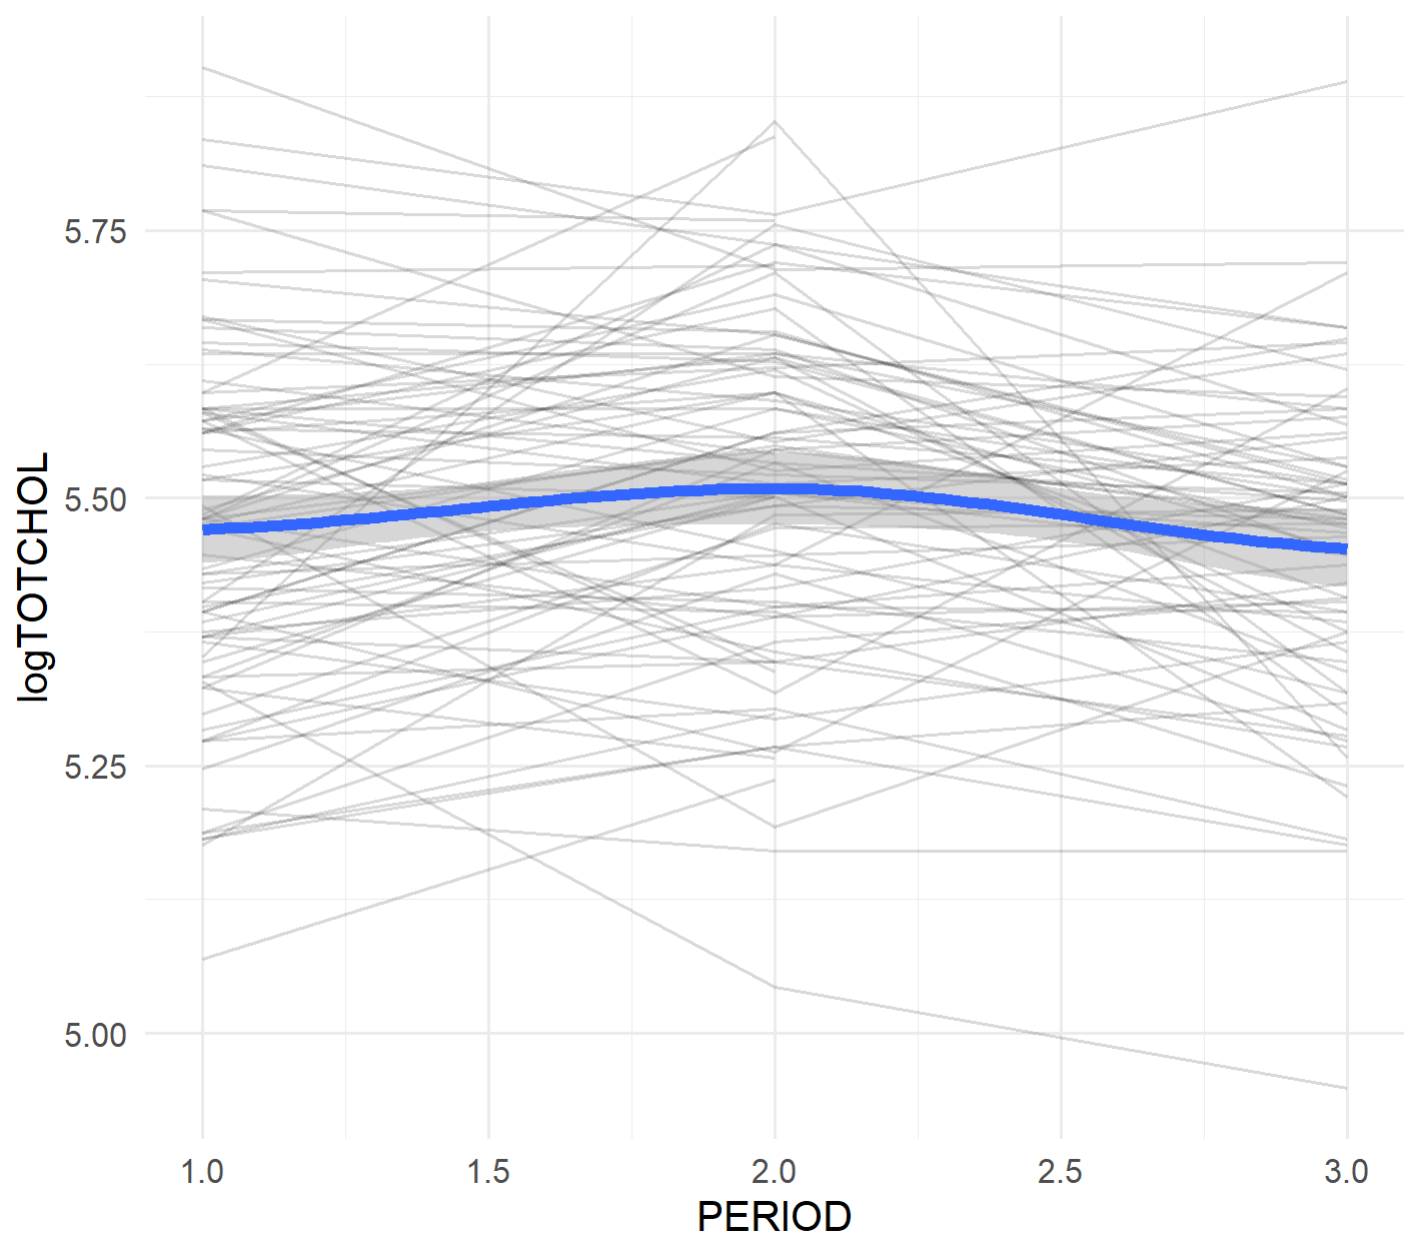
\includegraphics[width=0.8\textwidth]{figs/hw7_trajectory_plot.png}
\end{center}

从图中可以看出，胆固醇水平（取对数）随时间大致稳定，呈现先轻微上升后轻微下降的规律，视觉上并不十分明显，因此进一步进行分析。为了减少线性项和二次项之间的共线性，对 PERIOD 进行中心化处理 \texttt{period\_c=PERIOD-2}，随后比较 linear model 和 quadratic model，结果显示 likelihood ratio test 的 ANOVA $p < 2.2\times 10^{-16}$，即便考虑模型复杂度的惩罚，采用 BIC 进行分析，结果亦有二次模型 BIC 数值更低。

\begin{center}
\begin{tabular}{lcc}
\toprule
 & df & BIC \\
\midrule
linear model & 8 & $-10129$ \\
quadratic model & 9 & $-10738$ \\
\bottomrule
\end{tabular}
\end{center}

以上说明引入二次项可以显著改善模型拟合，因此后续分析中采用 quadratic model。

\item \textbf{LMM}（Linear Mixed Model）

\begin{center}
\small
\begin{tabular}{lcccccc}
\toprule
term & estimate & std.error & statistic & conf.low & conf.high \\
\midrule
(Intercept) & 5.2746 & 0.0144 & 365.496 & 5.2464 & 5.3029 \\
BMI & 0.0076 & 0.0005 & 14.581 & 0.0066 & 0.0087 \\
period\_c & 0.0019 & 0.0016 & 1.182 & $-0.0012$ & 0.0050 \\
I(period\_c$^2$) & $-0.0545$ & 0.0021 & $-25.681$ & $-0.0587$ & $-0.0504$ \\
AGE\_group2 & 0.0110 & 0.0034 & 3.254 & 0.0044 & 0.0177 \\
AGE\_group3 & $-0.0137$ & 0.0054 & $-2.530$ & $-0.0244$ & $-0.0031$ \\
SEX1 & 0.0558 & 0.0051 & 10.852 & 0.0458 & 0.0659 \\
\bottomrule
\end{tabular}
\end{center}

从表中我们可以看出，胆固醇水平与 BMI 显著正相关，且 PERIOD（二次项）、SEX 等协变量均对胆固醇水平有显著影响。

此外，random intercept 的标准差约为 0.15，说明不同个体间存在较为明显的异质性，这也验证了引入 random intercept 是合理的。

\item \textbf{GLMM}（Generalized Linear Mixed Model）

在 GLMM 中，我们将胆固醇状态定义为二分类变量，应用 logit 连接函数（\texttt{family = binomial}）。

\begin{center}
\small
\begin{tabular}{lcccccc}
\toprule
term & estimate & std.error & statistic & p.value & conf.low & conf.high \\
\midrule
(Intercept) & 1.9051 & 0.4757 & 4.0046 & 0.0001 & 0.9727 & 2.8375 \\
BMI & 0.1037 & 0.0175 & 5.9120 & 0.0000 & 0.0693 & 0.1381 \\
period\_c & $-0.0446$ & 0.0538 & $-0.8281$ & 0.4076 & $-0.1500$ & 0.0609 \\
I(period\_c$^2$) & $-1.4173$ & 0.0901 & $-15.7298$ & 0.0000 & $-1.5939$ & $-1.2407$ \\
AGE\_group2 & 0.4776 & 0.1281 & 3.7295 & 0.0002 & 0.2266 & 0.7286 \\
AGE\_group3 & $-0.1905$ & 0.1922 & $-0.9912$ & 0.3216 & $-0.5673$ & 0.1862 \\
SEX1 & 0.2741 & 0.1587 & 1.7272 & 0.0841 & $-0.0369$ & 0.5852 \\
\bottomrule
\end{tabular}
\end{center}

从表中我们可以看出，在同一个个体内，BMI 与不良胆固醇状态正相关，且 BMI 每增加 1 个单位，undesirable cholesterol 的 odds 平均增加 $e^{0.1037}-1=0.147$ 倍。

\item \textbf{GEE}（Generalized Estimating Equations）

\begin{center}
\small
\begin{tabular}{lcccccc}
\toprule
term & estimate & std.error & statistic & p.value & conf.low & conf.high \\
\midrule
(Intercept) & $-2.7736$ & 0.3042 & 83.1528 & 0.0000 & $-3.3698$ & $-2.1775$ \\
BMI & 0.0777 & 0.0100 & 60.8113 & 0.0000 & 0.0582 & 0.0973 \\
PERIOD & 2.4331 & 0.1806 & 181.5561 & 0.0000 & 2.0792 & 2.7870 \\
I(PERIOD$^2$) & $-0.6079$ & 0.0453 & 179.7287 & 0.0000 & $-0.6968$ & $-0.5190$ \\
AGE\_group2 & 0.2993 & 0.0573 & 27.2769 & 0.0000 & 0.1870 & 0.4116 \\
AGE\_group3 & 0.0318 & 0.0831 & 0.1466 & 0.7018 & $-0.1311$ & 0.1948 \\
SEX1 & 0.3851 & 0.0666 & 33.4689 & 0.0000 & 0.2546 & 0.5156 \\
\bottomrule
\end{tabular}
\end{center}

在 GEE 中，总体平均意义下，BMI 每增加一个单位，undesirable cholesterol 的 odds 平均增加约 0.0808 倍。

\item 如上可见，虽然二者的系数均为正，说明 BMI 与不良胆固醇状态呈现正相关，但 GLMM 的系数明显大于 GEE 的系数。这是因为 GLMM 研究的是同一个个体的 BMI 变化对胆固醇状态的影响，而 GEE 给出了总体平均意义下二者的关系。由于 GLMM 有 conditioning on random effects，去除了个体间异质性，因此 subject-specific association 通常比 marginal association 强，回归结果是合理的。
\end{enumerate}

\bigskip
\textbf{所用代码：}

\begin{lstlisting}
library(lme4)
library(geepack)
library(ggplot2)
library(dplyr)

df <- read.csv("Framingham_data.csv")

df$bi_chole <- ifelse(df$TOTCHOL > 200, 1, 0)
df$logTOTCHOL <- log(df$TOTCHOL)
df$SEX <- factor(df$SEX)
df$AGE_group <- factor(df$AGE_group)

dfclean <- na.omit(df[, c(
  "RANDID","logTOTCHOL","BMI","PERIOD","AGE_group","SEX","bi_chole"
)])

# === (a) Trajectory Plot ===
set.seed(100)
sampleid <- sample(unique(df$RANDID), 100)
plot_data <- subset(df, RANDID %in% sampleid & !is.na(logTOTCHOL))

ggplot(plot_data, aes(x=PERIOD, y=logTOTCHOL, group=RANDID)) +
  geom_line(alpha=0.15) +
  geom_smooth(aes(group=1), method="loess", linewidth=1.5) +
  theme_minimal()

# Model comparison: linear vs quadratic
dfclean$period_c <- as.numeric(dfclean$PERIOD) - 2
lmm_linear <- lmer(logTOTCHOL ~ BMI + as.numeric(period_c) + SEX +
                     factor(AGE_group) + (1|RANDID), data=dfclean)
lmm_quad <- lmer(logTOTCHOL ~ BMI + as.numeric(period_c) +
                   I(as.numeric(period_c)^2) + SEX + factor(AGE_group) +
                   (1|RANDID), data=dfclean)
anova(lmm_linear, lmm_quad)
BIC(lmm_linear, lmm_quad)

# === (b) LMM ===
library(broom.mixed)
library(knitr)

lmm_c <- lmer(
  logTOTCHOL ~ BMI + period_c + I(period_c^2) +
    AGE_group + SEX + (1 | RANDID),
  data = dfclean
)
tidy(lmm_c, conf.int = TRUE) %>% kable()

# === (c) GLMM ===
glmm <- glmer(
  bi_chole ~ BMI + period_c + I(period_c^2) +
    AGE_group + SEX + (1 | RANDID),
  data = dfclean, family = binomial
)
tidy(glmm, conf.int = TRUE) %>% kable()

# === (d) GEE ===
gee <- geeglm(
  bi_chole ~ BMI + PERIOD + I(PERIOD^2) +
    AGE_group + SEX,
  id = RANDID, data = dfclean,
  family = binomial, corstr = "exchangeable"
)
tidy(gee, conf.int = TRUE) %>% kable()
\end{lstlisting}

\newpage

%% ===== HW8 =====
\section{Homework 8: Survival Analysis}
% ============================================================
% Problem 1
% ============================================================
\subsection{Problem 1}

\begin{enumerate}

\item When no censoring occurs, the K-M curve is the complement of the empirical distribution function of the time variable $T$:
\[
\widehat{S}(t) = 1 - F_n(t).
\]

\textbf{Proof.}

由于无 Censoring，故 $d_i = 1$，且 $n_{i+1} = n_i - 1$，$\forall\, i$。

设 $T \le t$ 后有 $k$ 人存活，则
\[
\widehat{S}(t) = \prod_{t_i \le t}\!\left(1 - \frac{d_i}{n_i}\right)
= \prod_{t_i \le t} \frac{n_i - d_i}{n_i}
= \prod_{t_i \le t} \frac{n_i - i}{n_i - i + 1}
= \frac{n - k}{n}.
\]

又已知经验分布函数
\[
F_n(t) = \frac{1}{n}\sum_{i=1}^{n} \mathbf{1}_{\{T_i \le t\}} = \frac{k}{n},
\]
因此
\[
1 - F_n(t) = \frac{n-k}{n} = \widehat{S}(t). \qedhere
\]
\end{enumerate}

% ============================================================
% Problem 2
% ============================================================
\subsection{Problem 2}

\begin{enumerate}
\item The probability density function of the Pareto distribution is:
\[
f(t) = \begin{cases} \dfrac{p\,\theta^p}{t^{p+1}}, & t \ge \theta, \\[6pt] 0, & t < \theta, \end{cases}
\]
where $p > 0$ is a shape parameter and $\theta > 0$ is a scale parameter. Find its hazard function and survival function.

\textbf{Solution.}

\textbf{1. Survival function $S(t)$.}

当 $t < \theta$ 时，$S(t) = 1$；

当 $t \ge \theta$ 时，
\[
S(t) = \int_t^{+\infty} \frac{p\,\theta^p}{s^{p+1}}\,ds
= -\theta^p \cdot s^{-p}\Big|_t^{+\infty}
= \theta^p \cdot t^{-p} = \left(\frac{\theta}{t}\right)^p.
\]

综上：
\[
\boxed{S(t) = \begin{cases} 1, & t < \theta, \\[4pt] \left(\dfrac{\theta}{t}\right)^p, & t \ge \theta. \end{cases}}
\]

\textbf{2. Hazard function $h(t)$.}

由 $h(t) = \dfrac{f(t)}{S(t)}$，当 $t \ge \theta$ 时：
\[
h(t) = \frac{\dfrac{p\,\theta^p}{t^{p+1}}}{\left(\dfrac{\theta}{t}\right)^p} = \frac{p}{t}.
\]

综上：
\[
\boxed{h(t) = \begin{cases} 0, & t < \theta, \\[4pt] \dfrac{p}{t}, & t \ge \theta. \end{cases}}
\]
\end{enumerate}

% ============================================================
% Problem 3
% ============================================================
\subsection{Problem 3}

\begin{enumerate}
\item Show that the conditional likelihood for 1:1 binary matched-pair data equals the stratified partial likelihood, where each matched pair forms a stratum, the $Y=1$ observation is treated as an event and the $Y=0$ sample is treated as a censored observation.

\textbf{Proof.}

\textbf{(i) Conditional likelihood.}

对于 1:1 matched pair，设有 $n$ 对，每对有一个 $Y=0$ 和一个 $Y=1$，记为 $(X_{i1}, X_{i0})$，$Y_{i1}=1$，$Y_{i0}=0$，对应潜变量 $\alpha_i$。

利用 logistic regression 模型，第 $i$ 对的条件似然为
{\small
\[
L_i = P(Y_{i1}=1 \mid Y_{i1}+Y_{i0}=1)
= \frac{e^{\alpha_i + \beta^\top X_{i1}}}{e^{\alpha_i + \beta^\top X_{i1}} + e^{\alpha_i + \beta^\top X_{i0}}}
= \frac{e^{\beta^\top X_{i1}}}{e^{\beta^\top X_{i1}} + e^{\beta^\top X_{i0}}}.
\]
}

因此条件似然为
\[
\boxed{L_{\text{cond}} = \prod_{i=1}^{n} \frac{e^{\beta^\top X_{i1}}}{e^{\beta^\top X_{i1}} + e^{\beta^\top X_{i0}}}.} \tag{1}
\]

\textbf{(ii) Stratified partial likelihood.}

认为每一组（对）是一层，一层 2 个样本。记风险集 $\mathcal{R}_i$ 包含第 $i$ 对的两个个体，则分层偏似然中第 $i$ 层的贡献为
{\small
\[
L_i' = \frac{\lambda_0(t_i)e^{\beta^\top X_{i1}}}{\lambda_0(t_i)e^{\beta^\top X_{i1}} + \lambda_0(t_i)e^{\beta^\top X_{i0}}}
= \frac{e^{\beta^\top X_{i1}}}{e^{\beta^\top X_{i1}} + e^{\beta^\top X_{i0}}}.
\]
}

因此偏似然为
\[
\boxed{L_{\text{partial}} = \prod_{i=1}^{n} \frac{e^{\beta^\top X_{\text{event}}}}{\sum_{j \in \mathcal{R}_i} e^{\beta^\top X_{ij}}}
= \prod_{i=1}^{n} \frac{e^{\beta^\top X_{i1}}}{e^{\beta^\top X_{i1}} + e^{\beta^\top X_{i0}}}.} \tag{2}
\]

由 (1) $=$ (2)，即在本题所给条件下，二者等价。 \qedhere
\end{enumerate}

% ============================================================
% Problem 4
% ============================================================
\subsection{Problem 4}

\begin{enumerate}
\item \textbf{(Framingham Data)} The objective of this analysis is to examine the association between baseline BMI measurements and survival (assessed using the variables TIMEDTH and DEATH). Since we are interested in predictors of survival from the baseline examination, you may subset the dataset to include only PERIOD~1 data prior to conducting the analysis.

\begin{enumerate}[label=(\alph*)]
\item Previous studies have reported a U-shaped association between BMI and survival, where both low and high BMI are associated with poorer survival outcomes, while normal BMI correlates with the best survival.

\begin{enumerate}[label=\roman*.]
\item How many missing values are present in the BMI data? Compare the survival curves between participants with missing BMI values and those with complete data to answer the question: is the BMI data missing at random?

\textbf{Solution.}

用 \texttt{subset(df, PERIOD == 1)} 取出 PERIOD=1 的个体。

4215 个样本中存在 17 个 missing value。对比生存曲线可以发现 missing BMI 和记录 BMI 的个体生存曲线有较大差异，missing 的样本生存时间显著短于记录组（$H_0$：生存函数相同，$p\text{-value} < 0.0001$，拒绝 $H_0$）。

这说明该缺失不满足完全随机缺失假设，缺失本身携带了与高死亡风险相关的潜在信息。因此，在后续分类分析中，将 ``Missing'' 保留为独立类别是合理且有必要的。

\begin{center}
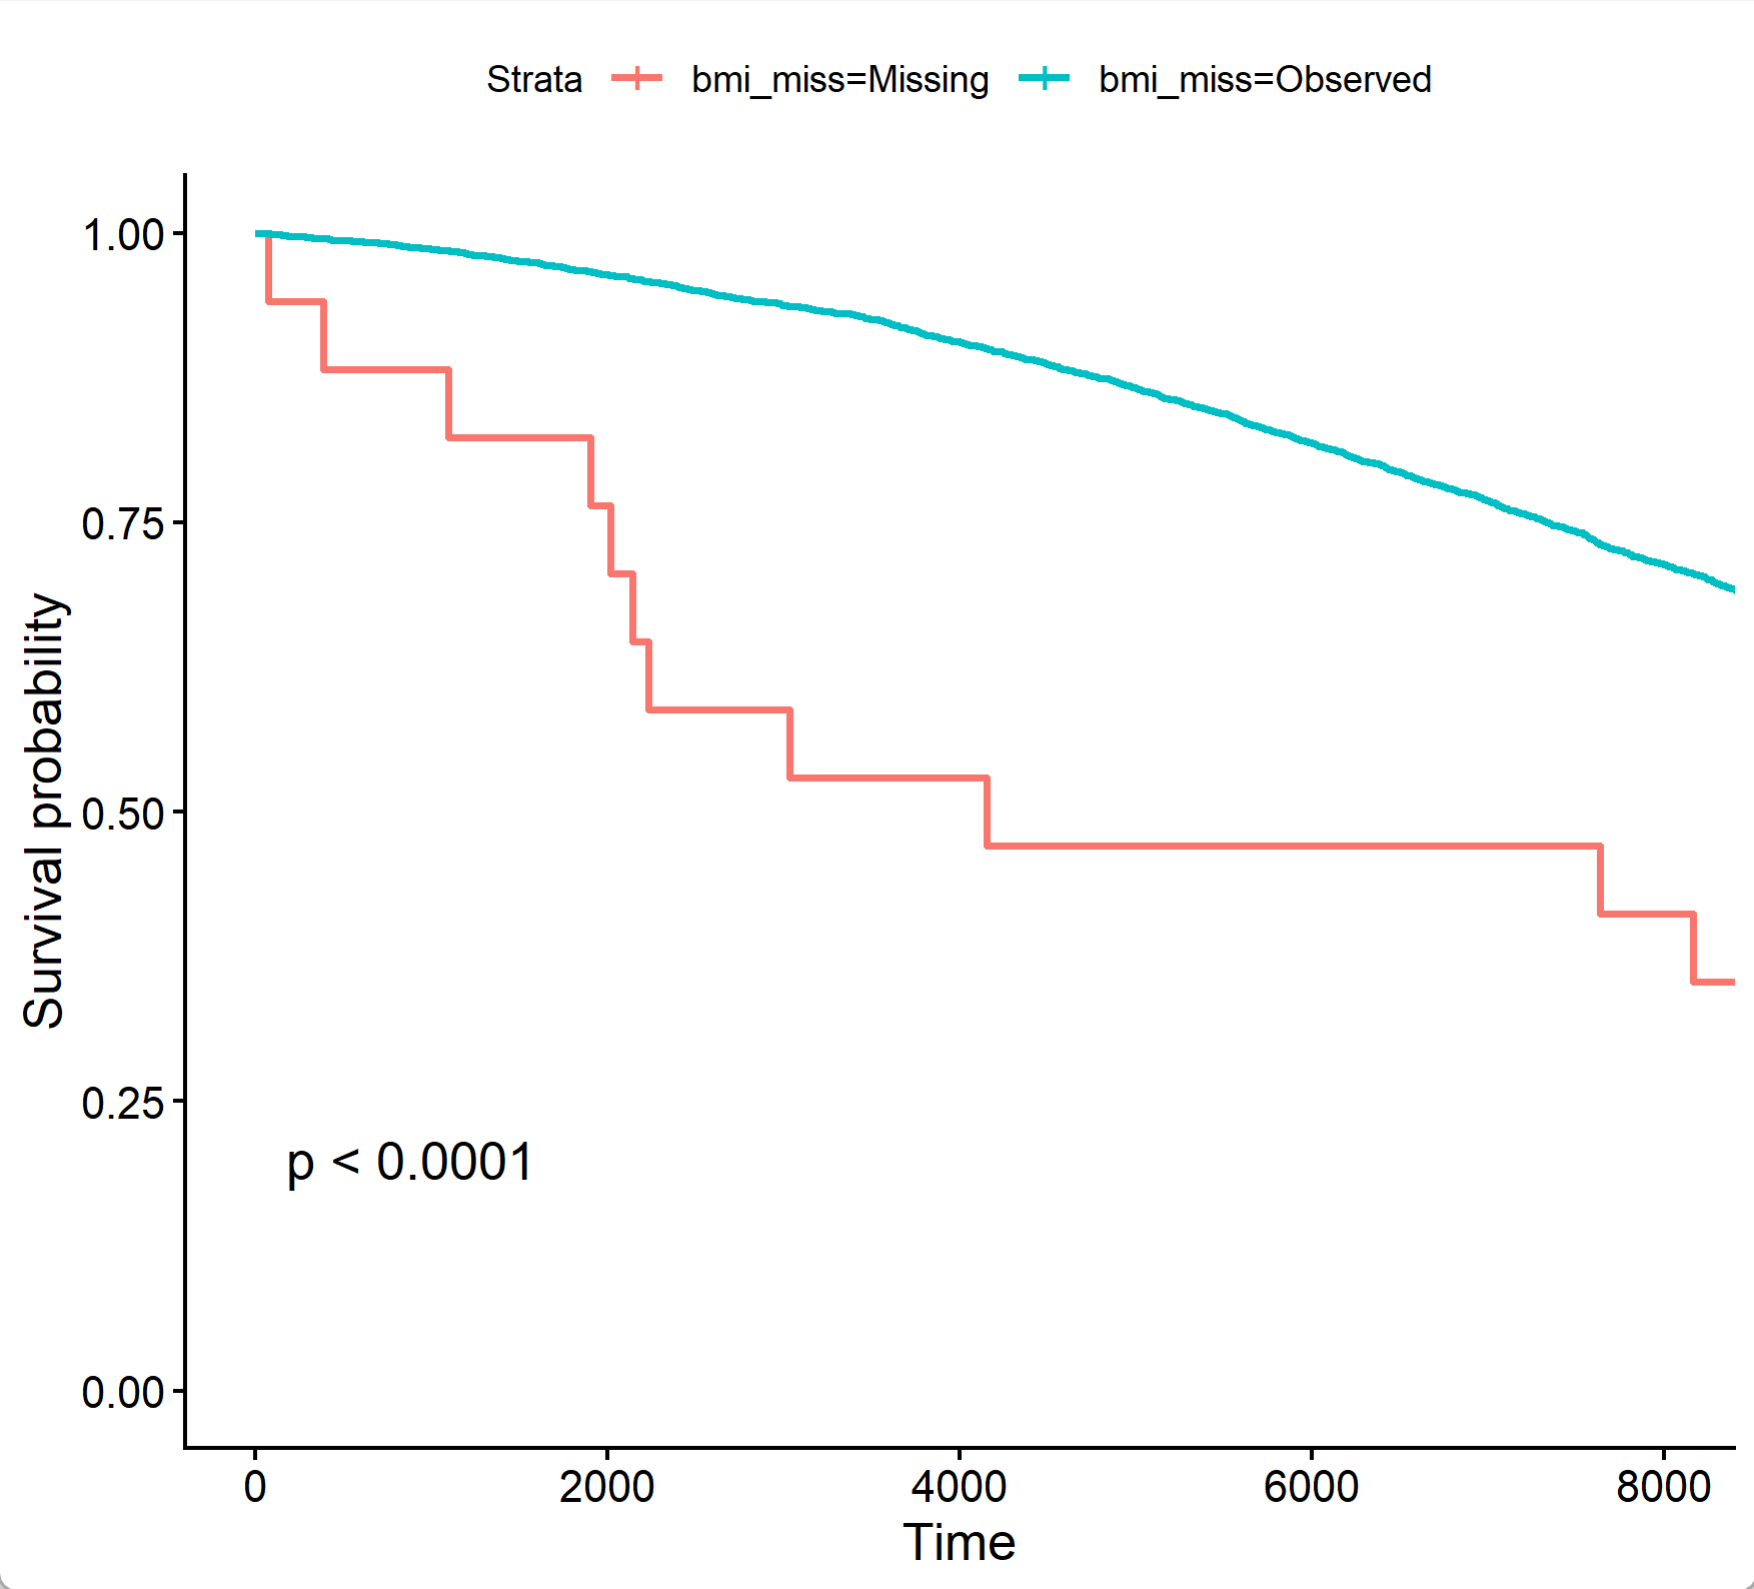
\includegraphics[width=0.7\textwidth]{figs/plot_missing_vs_observed.png}
\end{center}

\item Define a categorical ``weight'' variable: underweight if $\text{BMI} \in (0, 18.5)$; healthy weight if $\text{BMI} \in [18.5, 25)$; overweight if $\text{BMI} \in [25, 30)$; obese if $\text{BMI} \in [30, +\infty)$. If the BMI data is not missing at random, maintain missingness as a separate category. Visually compare survival curves across all categories (4 weight categories plus missing, if applicable). Do you observe the U-shape relationship between BMI and survival?

\textbf{Solution.}

\begin{center}
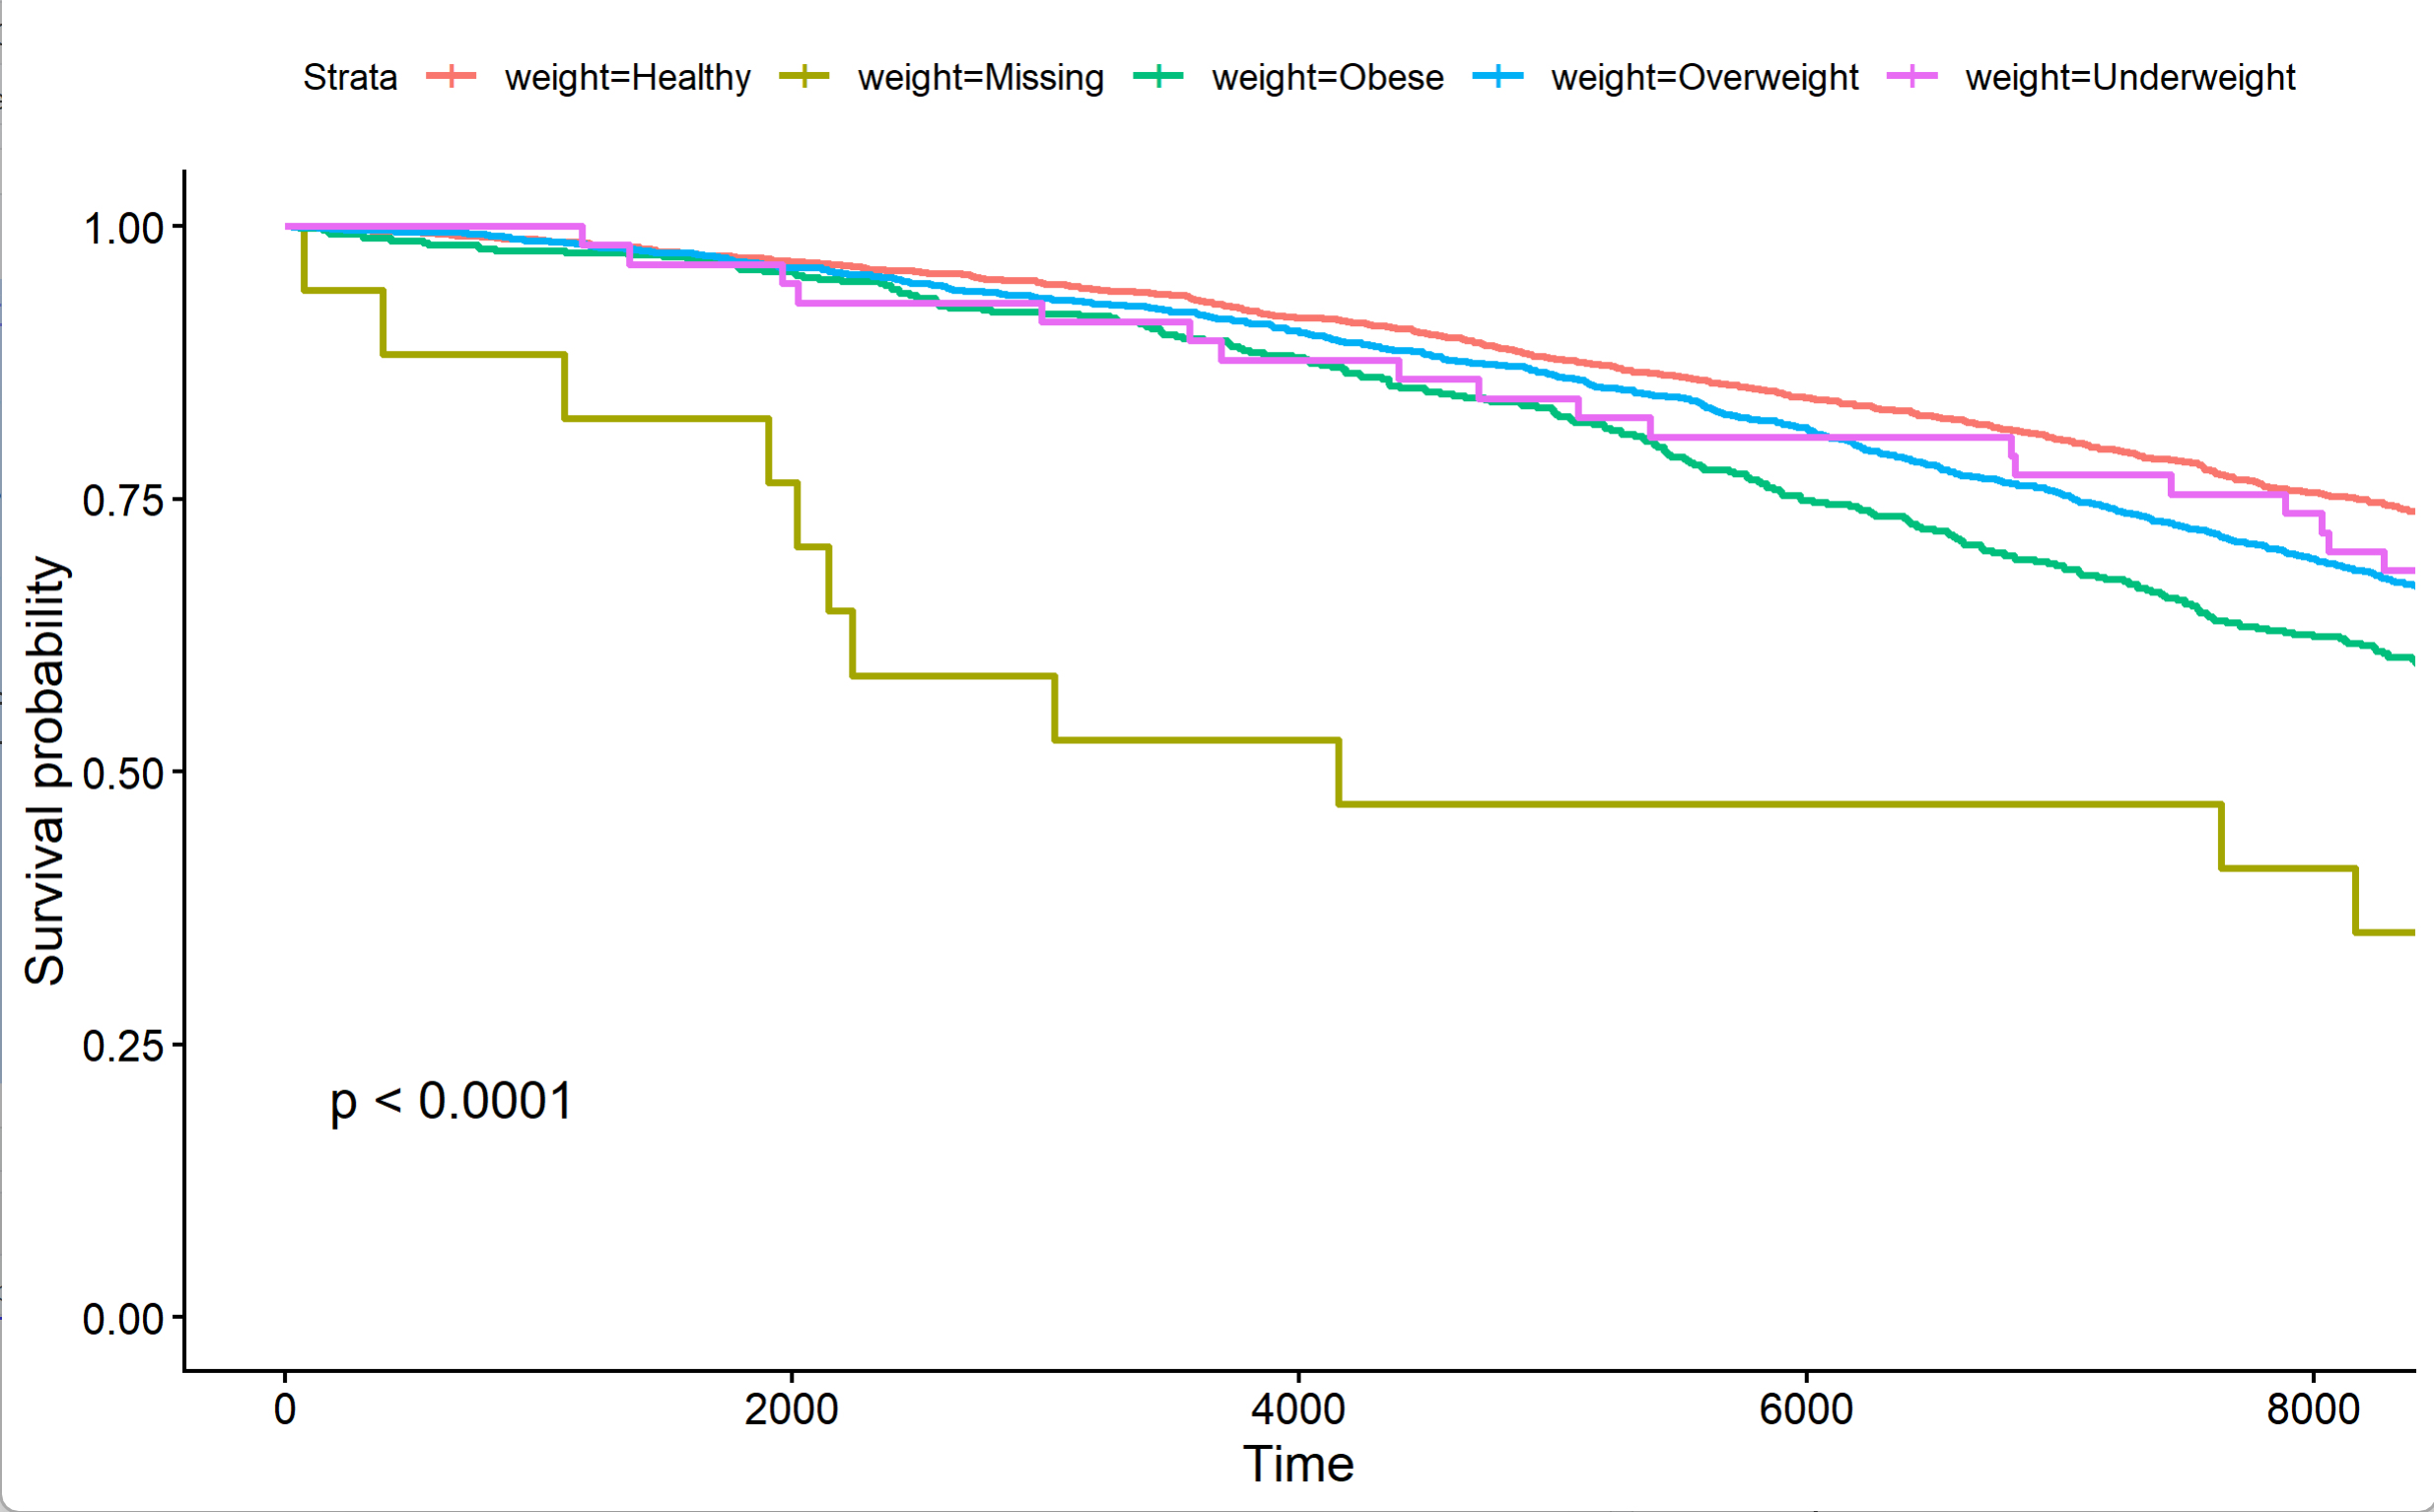
\includegraphics[width=0.7\textwidth]{figs/plot_weight_categories.png}
\end{center}

从生存曲线来看，各 BMI 组之间的生存概率存在一定差异。Healthy 组生存较好，而 Underweight 组生存曲线略低于 Healthy 组，Overweight、Obese 组的生存曲线也低于 Healthy Weight 组且 Obese 更低，可以说看出了``U''型。（但组间差异相对于与 Missing 组对比，肉眼来看并非十分明显。这启发了我们继续完成第二问的 Cox 模型。）

\item Can you find the median survival time for each weight category (excluding the missing category)? Why?

\textbf{Solution.}

无法找到。在本数据中，各 BMI 组的 Kaplan--Meier 生存曲线在随访结束时均未下降至 $0.5$，因此中位生存时间无法估计，或者说研究期间超过一半的受试者仍然存活，因此无法观察到中位生存时间。
\end{enumerate}

\item Investigate the association between baseline BMI (continuous) and survival using Cox regression, adjusted for sex, age group at baseline, baseline (log-transformed) glucose level, baseline hypertension status, baseline smoking status, and baseline total cholesterol. For BMI, subtract 25 to make it center at 25. Recentering is important to minimize the impact of multicollinearity since we may include the quadratic term due to the U-shape effect. Also include a quadratic term of baseline (log-transformed) glucose level, and the interaction between baseline hypertension and age group.

\begin{enumerate}[label=\roman*.]
\item Is there any evidence of the U-shape relationship between BMI and survival? Interpret BMI coefficients if they are significant.

\textbf{Solution.}

为研究基线 BMI 与死亡风险之间的关系，采用 Cox 比例风险模型对生存数据进行分析。将 BMI 以 $25\;\text{kg/m}^2$ 为中心进行中心化处理，引入中心化 BMI 的二次项以检验 BMI 与死亡风险之间可能存在的非线性关系。此外，模型还控制了性别（SEX）、年龄分组（AGE\_group，视为类别变量）、对数血糖（logglu）及其二次项（logglu2）、高血压状态（PREVHYP）、吸烟状态（CURSMOKE）、总胆固醇（TOTCHOL）以及年龄与高血压的交互项。分析采用完整案例（complete case）数据进行。

\begin{center}
\footnotesize
\begin{tabular}{lccccccc}
\toprule
Variable & coef & exp(coef) & se(coef) & $z$ & $\Pr(>|z|)$ & lower .95 & upper .95 \\
\midrule
BMIcenter        & $-0.0080$ & $0.9921$ & $0.0093$ & $-0.8563$ & $0.3919$ & $0.9741$ & $1.0103$ \\
BMIcenter2       & $0.0018$  & $1.0018$ & $0.0007$ & $2.5142$  & $0.0119$ & $1.0004$ & $1.0033$ \\
SEX              & $-0.5460$ & $0.5793$ & $0.0610$ & $-8.9533$ & $0.0000$ & $0.5140$ & $0.6528$ \\
AGE\_group2      & $1.1423$  & $3.1339$ & $0.0837$ & $13.6531$ & $0.0000$ & $2.6599$ & $3.6923$ \\
AGE\_group3      & $2.3105$  & $10.0792$& $0.1804$ & $12.8044$ & $0.0000$ & $7.0767$ & $14.3555$\\
logglu           & $-4.3704$ & $0.0126$ & $1.5485$ & $-2.8223$ & $0.0048$ & $0.0006$ & $0.2631$ \\
logglu2          & $0.5515$  & $1.7359$ & $0.1619$ & $3.4064$  & $0.0007$ & $1.2639$ & $2.3842$ \\
PREVHYP1         & $0.7509$  & $2.1190$ & $0.0857$ & $8.7658$  & $0.0000$ & $1.7915$ & $2.5064$ \\
CURSMOKE         & $0.2858$  & $1.3308$ & $0.0602$ & $4.7504$  & $0.0000$ & $1.1828$ & $1.4974$ \\
TOTCHOL          & $0.0017$  & $1.0017$ & $0.0006$ & $2.7212$  & $0.0065$ & $1.0005$ & $1.0030$ \\
AGE\_group2:PREVHYP1 & $-0.1196$ & $0.8872$ & $0.1200$ & $-0.9971$ & $0.3187$ & $0.7013$ & $1.1225$ \\
AGE\_group3:PREVHYP1 & $-0.6201$ & $0.5379$ & $0.2333$ & $-2.6580$ & $0.0079$ & $0.3405$ & $0.8497$ \\
\bottomrule
\end{tabular}
\end{center}

BMI 的线性项系数为 $-0.00797$（$p=0.392$），统计学不显著；而 BMI 的二次项系数为 $0.00183$（$p=0.012$），统计学显著。这表明 BMI 与死亡风险之间呈现出显著的二次曲线关系。由于二次项系数大于零，因此风险函数呈开口向上的形状，即存在 U 型关系：数学计算最低风险对应的 BMI 约为 $27.2\;\text{kg/m}^2$，而随着 BMI 偏离，无论是向较高还是较低方向，死亡风险均会增加，这和流行病学研究中观察到的 BMI 与死亡率间的 U 型关系是一致的。

\item Interpret the interactions between baseline hypertension and age group, if any interaction is significant.

\textbf{Solution.}

``In the absence of interactions, the predictors act additively on the log hazard.''

\begin{itemize}
\item 最年轻组内（AGE\_group=1，此组为参考组，后续 Hazard Ratio 都是与本组相比），组内高血压人群的 Hazard 是无高血压人群的 Hazard 的 $2.119$ 倍。
\item 年龄组 2（中年组）与高血压的交互项不显著（$p=0.3187$），说明该年龄组中高血压效应与参考组相比无显著差异。$\text{HR} = 2.1190 \times 0.8872 = 1.8800$。
\item 年龄组 3（老年组）与高血压的交互项显著（$\text{coef}=-0.6201$，$p=0.0079$），说明高血压效应仍然增加死亡风险但影响程度显著弱于年轻组。$\text{HR} = 1.1398$，即组内高血压人群的 Hazard 是无高血压人群的 Hazard 的 $1.1398$ 倍。
\end{itemize}
\end{enumerate}
\end{enumerate}

% ============================================================
% Appendix: R Code
% ============================================================
\newpage
\subsection*{Appendix: R Code}

\begin{lstlisting}[language=R, caption={HW8 R Code}]
library(survminer)
library(survival)
library(knitr)
#================
# (a)
#================
df <- read.csv("Framingham_data.csv")
# i
df1 <- subset(df, PERIOD == 1)
df1$bmi_miss <- ifelse(is.na(df1$BMI),
                       "Missing",
                       "Observed")

fit2 <- survfit(Surv(TIMEDTH, DEATH) ~ bmi_miss, data = df1)

# plot
ggsurvplot(fit2, pval = TRUE)

fit <- survfit(
  Surv(TIMEDTH, DEATH) ~ bmi_miss,
  data = df1
)

ggsurvplot(
  fit,
  pval=TRUE
)

survdiff(
  Surv(TIMEDTH,DEATH)~bmi_miss,
  data=df1
)

# ii
df1$weight <- cut(
  df1$BMI,
  breaks=c(0,18.5,25,30,Inf),
  labels=c(
    "Underweight",
    "Healthy",
    "Overweight",
    "Obese"
  ),
  right=FALSE
)
df1$weight <- as.character(df1$weight)

df1$weight[is.na(df1$BMI)] <- "Missing"

df1$weight <- factor(df1$weight)

fit2 <- survfit(
  Surv(TIMEDTH,DEATH)~weight,
  data=df1
)

ggsurvplot(
  fit2,
  pval=TRUE
)

#================
# (b)
#================
# data processing
df1$BMIcenter <- df1$BMI - 25 # recenter
df1$BMIcenter2 <- df1$BMIcenter^2
df1$logglu <- log(df1$GLUCOSE)
df1$logglu2 <- df1$logglu^2
df1$AGE_group <- as.factor(df1$AGE_group)
df1$PREVHYP <- as.factor(df1$PREVHYP)

# cox
coxfit <- coxph(
  Surv(TIMEDTH,DEATH)~
    BMIcenter+
    BMIcenter2+
    SEX+
    AGE_group+
    logglu+
    logglu2+
    PREVHYP+
    CURSMOKE+
    TOTCHOL+
    PREVHYP:AGE_group,
  data=df1
)

kable(cbind(as.data.frame(summary(coxfit)$coef),
            summary(coxfit)$conf[,3:4]),
      format="markdown", digits=4)
\end{lstlisting}
\end{enumerate}

\newpage

%% ===== HW9 =====
\section{Homework 9: Multiple Testing}
略。

\end{document}
